% Generated from Markdown by scripts/build_revision_v7_publication.py; do not edit numeric content manually.
% Options for packages loaded elsewhere
\PassOptionsToPackage{unicode}{hyperref}
\PassOptionsToPackage{hyphens}{url}
\PassOptionsToPackage{dvipsnames,svgnames,x11names}{xcolor}
\documentclass[
  10pt,
]{ctexart}
\usepackage{xcolor}
\usepackage[margin=18mm]{geometry}
\usepackage{amsmath,amssymb}
\setcounter{secnumdepth}{-\maxdimen} % remove section numbering
\usepackage{iftex}
\ifPDFTeX
  \usepackage[T1]{fontenc}
  \usepackage[utf8]{inputenc}
  \usepackage{textcomp} % provide euro and other symbols
\else % if luatex or xetex
  \usepackage{unicode-math} % this also loads fontspec
  \defaultfontfeatures{Scale=MatchLowercase}
  \defaultfontfeatures[\rmfamily]{Ligatures=TeX,Scale=1}
\fi
\usepackage{lmodern}
\ifPDFTeX\else
  % xetex/luatex font selection
\fi
% Use upquote if available, for straight quotes in verbatim environments
\IfFileExists{upquote.sty}{\usepackage{upquote}}{}
\IfFileExists{microtype.sty}{% use microtype if available
  \usepackage[]{microtype}
  \UseMicrotypeSet[protrusion]{basicmath} % disable protrusion for tt fonts
}{}
\makeatletter
\@ifundefined{KOMAClassName}{% if non-KOMA class
  \IfFileExists{parskip.sty}{%
    \usepackage{parskip}
  }{% else
    \setlength{\parindent}{0pt}
    \setlength{\parskip}{6pt plus 2pt minus 1pt}}
}{% if KOMA class
  \KOMAoptions{parskip=half}}
\makeatother
\usepackage{longtable,booktabs,array}
\newcounter{none} % for unnumbered tables
\usepackage{calc} % for calculating minipage widths
% Correct order of tables after \paragraph or \subparagraph
\usepackage{etoolbox}
\makeatletter
\patchcmd\longtable{\par}{\if@noskipsec\mbox{}\fi\par}{}{}
\makeatother
% Allow footnotes in longtable head/foot
\IfFileExists{footnotehyper.sty}{\usepackage{footnotehyper}}{\usepackage{footnote}}
\makesavenoteenv{longtable}
\usepackage{graphicx}
\makeatletter
\newsavebox\pandoc@box
\newcommand*\pandocbounded[1]{% scales image to fit in text height/width
  \sbox\pandoc@box{#1}%
  \Gscale@div\@tempa{\textheight}{\dimexpr\ht\pandoc@box+\dp\pandoc@box\relax}%
  \Gscale@div\@tempb{\linewidth}{\wd\pandoc@box}%
  \ifdim\@tempb\p@<\@tempa\p@\let\@tempa\@tempb\fi% select the smaller of both
  \ifdim\@tempa\p@<\p@\scalebox{\@tempa}{\usebox\pandoc@box}%
  \else\usebox{\pandoc@box}%
  \fi%
}
% Set default figure placement to htbp
\def\fps@figure{htbp}
\makeatother
% definitions for citeproc citations
\NewDocumentCommand\citeproctext{}{}
\NewDocumentCommand\citeproc{mm}{%
  \begingroup\def\citeproctext{#2}\cite{#1}\endgroup}
\makeatletter
 % allow citations to break across lines
 \let\@cite@ofmt\@firstofone
 % avoid brackets around text for \cite:
 \def\@biblabel#1{}
 \def\@cite#1#2{{#1\if@tempswa , #2\fi}}
\makeatother
\newlength{\cslhangindent}
\setlength{\cslhangindent}{1.5em}
\newlength{\csllabelwidth}
\setlength{\csllabelwidth}{3em}
\newenvironment{CSLReferences}[2] % #1 hanging-indent, #2 entry-spacing
 {\begin{list}{}{%
  \setlength{\itemindent}{0pt}
  \setlength{\leftmargin}{0pt}
  \setlength{\parsep}{0pt}
  % turn on hanging indent if param 1 is 1
  \ifodd #1
   \setlength{\leftmargin}{\cslhangindent}
   \setlength{\itemindent}{-1\cslhangindent}
  \fi
  % set entry spacing
  \setlength{\itemsep}{#2\baselineskip}}}
 {\end{list}}
\usepackage{calc}
\newcommand{\CSLBlock}[1]{\hfill\break\parbox[t]{\linewidth}{\strut\ignorespaces#1\strut}}
\newcommand{\CSLLeftMargin}[1]{\parbox[t]{\csllabelwidth}{\strut#1\strut}}
\newcommand{\CSLRightInline}[1]{\parbox[t]{\linewidth - \csllabelwidth}{\strut#1\strut}}
\newcommand{\CSLIndent}[1]{\hspace{\cslhangindent}#1}
\setlength{\emergencystretch}{3em} % prevent overfull lines
\providecommand{\tightlist}{%
  \setlength{\itemsep}{0pt}\setlength{\parskip}{0pt}}
\usepackage{bookmark}
\IfFileExists{xurl.sty}{\usepackage{xurl}}{} % add URL line breaks if available
\urlstyle{same}
\hypersetup{
  pdftitle={补充材料：NNS 计算图解释与 ViT 结构路径分析},
  colorlinks=true,
  linkcolor={Maroon},
  filecolor={Maroon},
  citecolor={Blue},
  urlcolor={Blue},
  pdfcreator={LaTeX via pandoc}}

\title{补充材料：NNS 计算图解释与 ViT 结构路径分析}
\author{}
\date{}

\begin{document}
\hypersetup{pdfauthor={},pdfsubject={},pdfkeywords={}}
\maketitle

\href{manuscript.md}{返回正文}。本文件包含复现参数、完整统计、历史图索引与后续实验范围。主文
RQ 编号按修订版使用。

\section{S1. Model and registry
details}\label{s1.-model-and-registry-details}

Models: \texttt{vit\_base\_patch16\_224.augreg2\_in21k\_ft\_in1k} and
\texttt{deit\_small\_patch16\_224.fb\_in1k}. Torch 2.2.2+cu121; timm
0.9.16; torchvision 0.17.2+cu121; NumPy 1.26.4; Pillow 10.2.0.

\refstepcounter{table}\label{tab:zh-supplement-001}
\textbf{Table S1. Original scalar registry coverage.}

{\def\LTcaptype{none} % do not increment counter
\begingroup\scriptsize
\setlength{\tabcolsep}{2pt}
\begin{longtable}[]{@{}
  >{\raggedright\arraybackslash}p{(\linewidth - 14\tabcolsep) * \real{0.1250}}
  >{\raggedright\arraybackslash}p{(\linewidth - 14\tabcolsep) * \real{0.1250}}
  >{\raggedright\arraybackslash}p{(\linewidth - 14\tabcolsep) * \real{0.1250}}
  >{\raggedright\arraybackslash}p{(\linewidth - 14\tabcolsep) * \real{0.1250}}
  >{\raggedright\arraybackslash}p{(\linewidth - 14\tabcolsep) * \real{0.1250}}
  >{\raggedright\arraybackslash}p{(\linewidth - 14\tabcolsep) * \real{0.1250}}
  >{\raggedright\arraybackslash}p{(\linewidth - 14\tabcolsep) * \real{0.1250}}
  >{\raggedright\arraybackslash}p{(\linewidth - 14\tabcolsep) * \real{0.1250}}@{}}
\toprule\noalign{}
\begin{minipage}[b]{\linewidth}\raggedright
Model
\end{minipage} & \begin{minipage}[b]{\linewidth}\raggedright
Object
\end{minipage} & \begin{minipage}[b]{\linewidth}\raggedright
Candidate definition
\end{minipage} & \begin{minipage}[b]{\linewidth}\raggedright
Candidates
\end{minipage} & \begin{minipage}[b]{\linewidth}\raggedright
Registered/image
\end{minipage} & \begin{minipage}[b]{\linewidth}\raggedright
Coverage
\end{minipage} & \begin{minipage}[b]{\linewidth}\raggedright
Strategy
\end{minipage} & \begin{minipage}[b]{\linewidth}\raggedright
Scalar neuron
\end{minipage} \\
\midrule\noalign{}
\endhead
\bottomrule\noalign{}
\endlastfoot
vit\_b16 & post-block token-channel & 12\emph{197}D & 1,815,552 & 192 &
0.01058\% & 12 blocks x 4 tokens x 4 channels & yes \\
vit\_b16 & post-block patch sum/energy & 2\emph{12}D & 18,432 & 96 &
0.52083\% & 12 blocks x 4 channels x 2 aggregates & no \\
vit\_b16 & attention-head coordinate & 12\emph{H}197*64 & 1,815,552 &
144 & 0.00793\% & all heads; CLS token; within-head channel 0 & yes \\
vit\_b16 & module patch aggregate & 3\emph{(4D+2}4D) & 27,648 & 18 &
0.06510\% & blocks 0/5/11; six modules; channel 0 & no \\
vit\_b16 & patch embedding aggregate & D & 768 & 4 & 0.52083\% & four
fixed channels; sum over patches & no \\
vit\_b16 & final CLS coordinate & D & 768 & 1 & 0.13021\% & channel 0 &
yes \\
vit\_b16 & ground-truth logit & 1000 & 1,000 & 1 & 0.10000\% & frozen
image label & output \\
vit\_b16 & clean-top1 logit & 1000 & 1,000 & 1 & 0.10000\% & frozen
clean prediction & output \\
deit\_s16 & post-block token-channel & 12\emph{197}D & 907,776 & 192 &
0.02115\% & 12 blocks x 4 tokens x 4 channels & yes \\
deit\_s16 & post-block patch sum/energy & 2\emph{12}D & 9,216 & 96 &
1.04167\% & 12 blocks x 4 channels x 2 aggregates & no \\
deit\_s16 & attention-head coordinate & 12\emph{H}197*64 & 907,776 & 72
& 0.00793\% & all heads; CLS token; within-head channel 0 & yes \\
deit\_s16 & module patch aggregate & 3\emph{(4D+2}4D) & 13,824 & 18 &
0.13021\% & blocks 0/5/11; six modules; channel 0 & no \\
deit\_s16 & patch embedding aggregate & D & 384 & 4 & 1.04167\% & four
fixed channels; sum over patches & no \\
deit\_s16 & final CLS coordinate & D & 384 & 1 & 0.26042\% & channel 0 &
yes \\
deit\_s16 & ground-truth logit & 1000 & 1,000 & 1 & 0.10000\% & frozen
image label & output \\
deit\_s16 & clean-top1 logit & 1000 & 1,000 & 1 & 0.10000\% & frozen
clean prediction & output \\
\end{longtable}
\endgroup
}

\refstepcounter{table}\label{tab:zh-supplement-002}
\textbf{Table S2. Resources and extended validation coverage.}

{\def\LTcaptype{none} % do not increment counter
\begingroup\scriptsize
\setlength{\tabcolsep}{2pt}
\begin{longtable}[]{@{}ll@{}}
\toprule\noalign{}
Resource / validation & Value \\
\midrule\noalign{}
\endhead
\bottomrule\noalign{}
\endlastfoot
Formal scan wall time & 1,752.71 s \\
Four-card GPU-hours upper bound & 1.9475 \\
Throughput & 192.16 targets/s \\
Retained data & 9.290 GB \\
Peak reserved GPU memory & 2.284 GB \\
Peak CPU RSS & 2.018 GB \\
M1 random permutations & 128,000,000 \\
M4 attention / residual / JVP records & 86,400 / 19,200 / 691,200 \\
\end{longtable}
\endgroup
}

\subsection{S1.1
实现与核心指标伪代码}\label{s1.1-ux5b9eux73b0ux4e0eux6838ux5fc3ux6307ux6807ux4f2aux4ee3ux7801}

模型均处于 evaluation mode。M3 使用 torch.autograd.grad 的
is\_grads\_batched 模式分块执行 VJP，冻结
gradient\_chunk\_size=16；具体随机种子、模型与图像哈希、worker
环境和每任务耗时记录在对应 evidence JSON
中。主扫描的时间、吞吐、显存与保留数据量见 Table S2；补充控制实验的 456
个任务合计 2.4502 GPU-hours。核心实现位于
src/vitnns/endpoint\_m3\_atlas.py、src/vitnns/endpoint\_m4.py 与相应
scripts/run\_endpoint\_*.py。

\begin{verbatim}
Endpoint(s, x):
    g <- VJP(s, x) at the observed forward state
    return x * g

StructuredCut(F, edges, reconstruction_target):
    for each actual use-edge z_k in a valid cut:
        g_k <- downstream cotangent dF/dz_k
        E_k <- x * VJP(z_k, x; vector=g_k)
    assert sum_k E_k closes to reconstruction_target # branch contribution or Total Endpoint

SpatialMetrics(E, target_patch):
    M[p] <- sum_rgb abs(E[p, rgb])
    if sum_p M[p] == 0: return NA
    p_patch <- patch_sum(M) / sum_p M[p]
    entropy <- -sum_j p_patch[j] log(p_patch[j]) / log(196)
    locality <- neighborhood_mass(target_patch) - uniform_neighborhood_mass
    distance <- sum_j p_patch[j] normalized_distance(j, target_patch)

RandomRegionAUC(repeats):
    for each random repeat r:
        curve_r <- absolute finite effect at every area budget
        auc_r <- trapezoid(curve_r, area in [0, 0.25]) / 0.25
    return mean_r auc_r
\end{verbatim}

CLS 没有自然的目标 patch，因此 locality 与 target-relative distance 仅对
patch-token 目标定义；零质量样本传播为 NA。图内 token、channel 与 head
先按预定规则汇总，再以图像为统计单位。

\section{S2. Frozen decisions and numerical
diagnostics}\label{s2.-frozen-decisions-and-numerical-diagnostics}

C4a: BROAD\_BUT\_NON\_UNIVERSAL\_FAMILY\_LEVEL\_SUPPORT; original
all-family omnibus NOT\_SUPPORTED. C4b: NOT\_SUPPORTED. The numerical
atlas status is
PASS\_FLOAT64\_RECOVERY\_WITH\_RETAINED\_FLOAT32\_FAILURE: 36/57,600
float32 failures are retained and 36/36 same-coordinate float64 checks
pass. These fields are not interchangeable.

\refstepcounter{table}\label{tab:zh-supplement-003}
\textbf{Table S2.1. 原 pooled C4a provenance；图像级中位数 {[}95\%
CI{]}。} Holm p 来自原成分和区域合计 28 项的冻结 family。

{\def\LTcaptype{none} % do not increment counter
\begingroup\scriptsize
\setlength{\tabcolsep}{2pt}
\begin{longtable}[]{@{}
  >{\raggedright\arraybackslash}p{(\linewidth - 8\tabcolsep) * \real{0.2000}}
  >{\raggedright\arraybackslash}p{(\linewidth - 8\tabcolsep) * \real{0.2000}}
  >{\raggedright\arraybackslash}p{(\linewidth - 8\tabcolsep) * \real{0.2000}}
  >{\raggedright\arraybackslash}p{(\linewidth - 8\tabcolsep) * \real{0.2000}}
  >{\raggedright\arraybackslash}p{(\linewidth - 8\tabcolsep) * \real{0.2000}}@{}}
\toprule\noalign{}
\begin{minipage}[b]{\linewidth}\raggedright
Model
\end{minipage} & \begin{minipage}[b]{\linewidth}\raggedright
Reference
\end{minipage} & \begin{minipage}[b]{\linewidth}\raggedright
Heads
\end{minipage} & \begin{minipage}[b]{\linewidth}\raggedright
A/V pooled
\end{minipage} & \begin{minipage}[b]{\linewidth}\raggedright
Residual pooled
\end{minipage} \\
\midrule\noalign{}
\endhead
\bottomrule\noalign{}
\endlastfoot
vit\_b16 & normalized-zero & 0.291 {[}0.281, 0.298{]} & 0.0996 {[}0.075,
0.123{]} & 0.177 {[}0.155, 0.195{]} \\
vit\_b16 & blur & 0.306 {[}0.296, 0.318{]} & 0.157 {[}0.131, 0.177{]} &
0.209 {[}0.182, 0.237{]} \\
deit\_s16 & normalized-zero & 0.191 {[}0.177, 0.205{]} & 0.107 {[}0.078,
0.129{]} & 0.135 {[}0.113, 0.164{]} \\
deit\_s16 & blur & 0.182 {[}0.168, 0.195{]} & 0.160 {[}0.128, 0.185{]} &
0.229 {[}0.204, 0.251{]} \\
\end{longtable}
\endgroup
}

12 项原 Holm 调整后 p 均小于 \(10^{-6}\)。原 composite 中 11/12 family
达到操作门槛，但 all-family C4a 仍为
\texttt{NOT\_SUPPORTED}。这张表保存历史判定身份；S18
的分层诊断不追溯改变它。

\section{S3. Reference sensitivity}\label{s3.-reference-sensitivity}

Change uses atol=1e-12 and rtol=0. Relative change is
abs(q0-qblur)/max(abs(q0),abs(qblur)); both-zero denominators are NA.
Component quantiles describe the pooled records, not independent
inferential samples.

\refstepcounter{table}\label{tab:zh-supplement-004}
\textbf{Table S3. Changes in Taylor magnitude and absolute finite
effect.}

{\def\LTcaptype{none} % do not increment counter
\begingroup\scriptsize
\setlength{\tabcolsep}{2pt}
\begin{longtable}[]{@{}
  >{\raggedright\arraybackslash}p{(\linewidth - 10\tabcolsep) * \real{0.1667}}
  >{\raggedright\arraybackslash}p{(\linewidth - 10\tabcolsep) * \real{0.1667}}
  >{\raggedright\arraybackslash}p{(\linewidth - 10\tabcolsep) * \real{0.1667}}
  >{\raggedright\arraybackslash}p{(\linewidth - 10\tabcolsep) * \real{0.1667}}
  >{\raggedright\arraybackslash}p{(\linewidth - 10\tabcolsep) * \real{0.1667}}
  >{\raggedright\arraybackslash}p{(\linewidth - 10\tabcolsep) * \real{0.1667}}@{}}
\toprule\noalign{}
\begin{minipage}[b]{\linewidth}\raggedright
Model
\end{minipage} & \begin{minipage}[b]{\linewidth}\raggedright
Quantity
\end{minipage} & \begin{minipage}[b]{\linewidth}\raggedright
Component pairs
\end{minipage} & \begin{minipage}[b]{\linewidth}\raggedright
Above tolerance
\end{minipage} & \begin{minipage}[b]{\linewidth}\raggedright
Abs change median {[}q10,q90{]}
\end{minipage} & \begin{minipage}[b]{\linewidth}\raggedright
Relative change median {[}q10,q90{]}
\end{minipage} \\
\midrule\noalign{}
\endhead
\bottomrule\noalign{}
\endlastfoot
DeiT-S/16 & finite\_effect & 67200 & 100.0\% & 0.1365 {[}0.0161,
1.6575{]} & 0.4927 {[}0.0985, 0.8997{]} \\
DeiT-S/16 & taylor & 67200 & 100.0\% & 0.1215 {[}0.0150, 0.7867{]} &
0.5186 {[}0.1172, 0.9033{]} \\
ViT-B/16 & finite\_effect & 96000 & 100.0\% & 0.0713 {[}0.0076,
1.4414{]} & 0.5300 {[}0.1117, 0.9137{]} \\
ViT-B/16 & taylor & 96000 & 100.0\% & 0.0688 {[}0.0078, 0.5471{]} &
0.5225 {[}0.1133, 0.9052{]} \\
\end{longtable}
\endgroup
}

Head rankings use average ranks and Kendall tau-b. Top-K ties are broken
by ascending component ID; Top-3 overlap is intersection size / 3. Rank
displacement uses original rank positions, so model head counts affect
its scale. Each image averages 12 blocks, then summaries use 400 images.
Full-order equality counts are Taylor 0/4,800 and effect 0/4,800 for
ViT-B, Taylor 46/4,800 and effect 64/4,800 for DeiT-S.

\refstepcounter{table}\label{tab:zh-supplement-005}
\textbf{Table S4. Image-level rank concordance distributions.}

{\def\LTcaptype{none} % do not increment counter
\begingroup\scriptsize
\setlength{\tabcolsep}{2pt}
\begin{longtable}[]{@{}
  >{\raggedright\arraybackslash}p{(\linewidth - 8\tabcolsep) * \real{0.2000}}
  >{\raggedright\arraybackslash}p{(\linewidth - 8\tabcolsep) * \real{0.2000}}
  >{\raggedright\arraybackslash}p{(\linewidth - 8\tabcolsep) * \real{0.2000}}
  >{\raggedright\arraybackslash}p{(\linewidth - 8\tabcolsep) * \real{0.2000}}
  >{\raggedright\arraybackslash}p{(\linewidth - 8\tabcolsep) * \real{0.2000}}@{}}
\toprule\noalign{}
\begin{minipage}[b]{\linewidth}\raggedright
Model
\end{minipage} & \begin{minipage}[b]{\linewidth}\raggedright
Quantity
\end{minipage} & \begin{minipage}[b]{\linewidth}\raggedright
Metric
\end{minipage} & \begin{minipage}[b]{\linewidth}\raggedright
Image median {[}q10,q90{]}
\end{minipage} & \begin{minipage}[b]{\linewidth}\raggedright
n / NA
\end{minipage} \\
\midrule\noalign{}
\endhead
\bottomrule\noalign{}
\endlastfoot
DeiT-S/16 & finite\_effect & spearman & 0.3071 {[}0.1238, 0.4524{]} &
400 / 0 \\
DeiT-S/16 & finite\_effect & kendall\_tau\_b & 0.2444 {[}0.0989,
0.3678{]} & 400 / 0 \\
DeiT-S/16 & finite\_effect & top1\_agreement & 0.4167 {[}0.1667,
0.5833{]} & 400 / 0 \\
DeiT-S/16 & finite\_effect & top3\_overlap & 0.6111 {[}0.5278, 0.6944{]}
& 400 / 0 \\
DeiT-S/16 & finite\_effect & mean\_absolute\_rank\_displacement & 1.5278
{[}1.2778, 1.7528{]} & 400 / 0 \\
DeiT-S/16 & taylor & spearman & 0.3000 {[}0.1000, 0.4476{]} & 400 / 0 \\
DeiT-S/16 & taylor & kendall\_tau\_b & 0.2389 {[}0.0778, 0.3667{]} & 400
/ 0 \\
DeiT-S/16 & taylor & top1\_agreement & 0.3333 {[}0.1667, 0.5833{]} & 400
/ 0 \\
DeiT-S/16 & taylor & top3\_overlap & 0.6111 {[}0.5278, 0.6944{]} & 400 /
0 \\
DeiT-S/16 & taylor & mean\_absolute\_rank\_displacement & 1.5278
{[}1.3056, 1.8056{]} & 400 / 0 \\
ViT-B/16 & finite\_effect & spearman & 0.3759 {[}0.2622, 0.4904{]} & 400
/ 0 \\
ViT-B/16 & finite\_effect & kendall\_tau\_b & 0.2803 {[}0.1967,
0.3740{]} & 400 / 0 \\
ViT-B/16 & finite\_effect & top1\_agreement & 0.3333 {[}0.2500,
0.5833{]} & 400 / 0 \\
ViT-B/16 & finite\_effect & top3\_overlap & 0.5000 {[}0.4167, 0.6111{]}
& 400 / 0 \\
ViT-B/16 & finite\_effect & mean\_absolute\_rank\_displacement & 2.9444
{[}2.6111, 3.2917{]} & 400 / 0 \\
ViT-B/16 & taylor & spearman & 0.3782 {[}0.2539, 0.4914{]} & 400 / 0 \\
ViT-B/16 & taylor & kendall\_tau\_b & 0.2828 {[}0.1942, 0.3737{]} & 400
/ 0 \\
ViT-B/16 & taylor & top1\_agreement & 0.3333 {[}0.2500, 0.5833{]} & 400
/ 0 \\
ViT-B/16 & taylor & top3\_overlap & 0.5000 {[}0.4167, 0.6111{]} & 400 /
0 \\
ViT-B/16 & taylor & mean\_absolute\_rank\_displacement & 2.9444
{[}2.5972, 3.2792{]} & 400 / 0 \\
\end{longtable}
\endgroup
}

\section{S4. Method objects}\label{s4.-method-objects}

\refstepcounter{table}\label{tab:zh-supplement-006}
\textbf{Table S5. Functional comparison.}

{\def\LTcaptype{none} % do not increment counter
\begingroup\scriptsize
\setlength{\tabcolsep}{2pt}
\begin{longtable}[]{@{}
  >{\raggedright\arraybackslash}p{(\linewidth - 6\tabcolsep) * \real{0.2500}}
  >{\raggedright\arraybackslash}p{(\linewidth - 6\tabcolsep) * \real{0.2500}}
  >{\raggedright\arraybackslash}p{(\linewidth - 6\tabcolsep) * \real{0.2500}}
  >{\raggedright\arraybackslash}p{(\linewidth - 6\tabcolsep) * \real{0.2500}}@{}}
\toprule\noalign{}
\begin{minipage}[b]{\linewidth}\raggedright
Method
\end{minipage} & \begin{minipage}[b]{\linewidth}\raggedright
Primary object
\end{minipage} & \begin{minipage}[b]{\linewidth}\raggedright
External reference
\end{minipage} & \begin{minipage}[b]{\linewidth}\raggedright
Propagation / contract
\end{minipage} \\
\midrule\noalign{}
\endhead
\bottomrule\noalign{}
\endlastfoot
Endpoint & Normalized-input Total Endpoint & No; normalization origin
matters & Global cuts close to total; branch partitions close to
branch \\
Activation-space Taylor & Specified replacement effect & Yes & Clean
cotangent × displacement \\
Integrated Gradients & Baseline-to-input attribution & Yes &
Path-average gradient; baseline-difference completeness \\
Attention rollout & Token flow & No & Accumulated attention / residual
flow \\
Grad-CAM & Class-conditioned coarse localization & No &
Gradient-weighted feature maps \\
Chefer / AttnLRP & Transformer relevance & Implementation-specific &
Method-specific relevance rules \\
Raw attention & Token allocation & No & Forward attention weights \\
\end{longtable}
\endgroup
}

\refstepcounter{table}\label{tab:zh-supplement-007}
\textbf{Table S5a. 完整近邻差分矩阵。}
``未报告''限于参考文献表所列核验版本；不同方法的 closure 对象不可互换。

{\def\LTcaptype{none} % do not increment counter
\begingroup\scriptsize
\setlength{\tabcolsep}{2pt}
\begin{longtable}[]{@{}
  >{\raggedright\arraybackslash}p{(\linewidth - 10\tabcolsep) * \real{0.1667}}
  >{\raggedright\arraybackslash}p{(\linewidth - 10\tabcolsep) * \real{0.1667}}
  >{\raggedright\arraybackslash}p{(\linewidth - 10\tabcolsep) * \real{0.1667}}
  >{\raggedright\arraybackslash}p{(\linewidth - 10\tabcolsep) * \real{0.1667}}
  >{\raggedright\arraybackslash}p{(\linewidth - 10\tabcolsep) * \real{0.1667}}
  >{\raggedright\arraybackslash}p{(\linewidth - 10\tabcolsep) * \real{0.1667}}@{}}
\toprule\noalign{}
\begin{minipage}[b]{\linewidth}\raggedright
Method family
\end{minipage} & \begin{minipage}[b]{\linewidth}\raggedright
Explained object
\end{minipage} & \begin{minipage}[b]{\linewidth}\raggedright
Consumer edge/use
\end{minipage} & \begin{minipage}[b]{\linewidth}\raggedright
Spatial component map
\end{minipage} & \begin{minipage}[b]{\linewidth}\raggedright
Closure object
\end{minipage} & \begin{minipage}[b]{\linewidth}\raggedright
Finite intervention
\end{minipage} \\
\midrule\noalign{}
\endhead
\bottomrule\noalign{}
\endlastfoot
Gradient × Input & 当前点输入加权梯度 & 未报告 & 单一输入图 &
一般不满足函数值完整性 & 否 \\
Integrated Gradients & reference-to-input 路径归因 & 未报告 & 单一输入图
& 输出差 & 否 \\
Conductance & 经过隐藏单元的路径归因 & 隐藏单元集合 & 可选输入分辨率 &
层级输出差 & 否 \\
GlobEnc / ALTI & 跨层 token contribution/mixing & 算子级 & token 图 &
局部前向分解 & 否 \\
DecompX & representation 与 logit 的 token components & 组件级 & token
分项 & 依 bias 分配规则重组 & 否 \\
AttnLRP / HiLRP / GradSkip & Transformer relevance & 算子连接 &
relevance 图 & relevance conservation & 否 \\
EAP / AtP* / Vi-CD & reference-specific component/edge effect & 是 &
通常不保留本文的输入坐标分项 & patching effect 或 circuit fidelity &
是 \\
Activation patching / CAAP & 内部 activation 替换效应 & node 或指定
activation & patch score & 一般不加和 & 是 \\
DAVE & ViT input-gradient 分解 & 未报告 consumer-use 索引 & 像素图 &
effective input-output map & 否 \\
Unpack & component interaction、命名路径与 token credit & 组件/路径身份
& token attribution & 方法特定 credit decomposition & 否 \\
NNS--ViT & 指定 use 与输入位置的同一当前点局部微分 &
consumer、slot、invocation & 分项输入图 & 声明 branch 或 global cut
的同一 signed differential & 分开评价 \\
\end{longtable}
\endgroup
}

\section{S4.1
中英术语合同}\label{s4.1-ux4e2dux82f1ux672fux8bedux5408ux540c}

{\def\LTcaptype{none} % do not increment counter
\begingroup\scriptsize
\setlength{\tabcolsep}{2pt}
\begin{longtable}[]{@{}
  >{\raggedright\arraybackslash}p{(\linewidth - 4\tabcolsep) * \real{0.3333}}
  >{\raggedright\arraybackslash}p{(\linewidth - 4\tabcolsep) * \real{0.3333}}
  >{\raggedright\arraybackslash}p{(\linewidth - 4\tabcolsep) * \real{0.3333}}@{}}
\toprule\noalign{}
\begin{minipage}[b]{\linewidth}\raggedright
中文
\end{minipage} & \begin{minipage}[b]{\linewidth}\raggedright
English
\end{minipage} & \begin{minipage}[b]{\linewidth}\raggedright
定义边界
\end{minipage} \\
\midrule\noalign{}
\endhead
\bottomrule\noalign{}
\endlastfoot
结构合法切面 & structurally valid cut & 每条输入到目标的结构 use-path
恰穿一次，与当前点数值无关 \\
点态微分闭合 & pointwise differential closure & 固定输入处 use-specific
Jacobian/cotangent 分组之和 \\
分支微分分组 & branch differential partition & 仅重构 attention 或 MLP
branch contribution \\
全局切面 & global cut & 包含 bypass 并重构同目标 Total Endpoint \\
路径图 & path map & 指定 tensor use 的局部微分分项，不是唯一因果路径 \\
局部微分绝对质量比 & local-differential absolute-mass ratio &
routing/identity scale；不是因果贡献率 \\
区域诱导的指定-head activation 替换 & region-induced replacement of
designated head activations & 混合输入产生 head activation，再插入 clean
forward 的两阶段任务 \\
候选集合遗憾率 & candidate-set regret &
相对已评价候选集合包络，不是全局最优策略 regret \\
\end{longtable}
\endgroup
}

\section{S5. Corrected absolute random AUC and
oracle}\label{s5.-corrected-absolute-random-auc-and-oracle}

当前随机基线对每次重复先取绝对值并积分，再平均 AUC。修正结果、重复分布和
MC 稳定性见\href{supplement_experiments_v1.md}{supplementary experiments
S9}. 旧分析作为原估计器的历史复核保留。

\section{S6. Detailed attention/residual evidence (historical stage
identifiers
retained)}\label{s6.-detailed-attentionresidual-evidence-historical-stage-identifiers-retained}

\subsection{历史 M4：Attention routing/value 与 residual
机制}\label{ux5386ux53f2-m4attention-routingvalue-ux4e0e-residual-ux673aux5236}

M4 完成两模型共享 400 图、12 个 blocks 和全部 heads 的
ground-truth-logit 局部输入依赖分解，共 86,400 个 image-block-head
attention records、19,200 个 image-block-residual records 和 691,200 个
direction-head JVP records。Q+K+V 逐 head 重构 native attention
Endpoint；routing+value 重构同一对象；attention 和 MLP residual 的
identity/carry 加 branch 均重构完整 logit Endpoint。

独立 CPU 审计复算 230,400 个 E3 summary 字段。最大 Q/K/V closure
绝对误差为 1.574e-05，最大 residual closure 绝对误差为 2.480e-05，显式
attention differential 与 native JVP 的最大相对误差为 2.502e-05。全部
19,200 个省略 identity/carry 负控按预期闭合失败；冻结前 16 个 evaluation
orders 的 384 个 attention-detach block checks 通过。

\subsubsection{Attention routing/value}\label{attention-routingvalue}

{\def\LTcaptype{none} % do not increment counter
\begingroup\scriptsize
\setlength{\tabcolsep}{2pt}
\begin{longtable}[]{@{}
  >{\raggedright\arraybackslash}p{(\linewidth - 12\tabcolsep) * \real{0.1111}}
  >{\raggedleft\arraybackslash}p{(\linewidth - 12\tabcolsep) * \real{0.1481}}
  >{\raggedleft\arraybackslash}p{(\linewidth - 12\tabcolsep) * \real{0.1481}}
  >{\raggedleft\arraybackslash}p{(\linewidth - 12\tabcolsep) * \real{0.1481}}
  >{\raggedleft\arraybackslash}p{(\linewidth - 12\tabcolsep) * \real{0.1481}}
  >{\raggedleft\arraybackslash}p{(\linewidth - 12\tabcolsep) * \real{0.1481}}
  >{\raggedleft\arraybackslash}p{(\linewidth - 12\tabcolsep) * \real{0.1481}}@{}}
\toprule\noalign{}
\begin{minipage}[b]{\linewidth}\raggedright
模型
\end{minipage} & \begin{minipage}[b]{\linewidth}\raggedleft
Block
\end{minipage} & \begin{minipage}[b]{\linewidth}\raggedleft
Routing share
\end{minipage} & \begin{minipage}[b]{\linewidth}\raggedleft
Frozen-attention Endpoint error
\end{minipage} & \begin{minipage}[b]{\linewidth}\raggedleft
Frozen-attention JVP error
\end{minipage} & \begin{minipage}[b]{\linewidth}\raggedleft
Mean-query saturation
\end{minipage} & \begin{minipage}[b]{\linewidth}\raggedleft
Routing-value path cancellation
\end{minipage} \\
\midrule\noalign{}
\endhead
\bottomrule\noalign{}
\endlastfoot
vit\_b16 & 0 & 0.3092 & 0.4407 & 0.4508 & 0.4656 & 0.1555 \\
vit\_b16 & 5 & 0.5239 & 0.7792 & 0.8547 & 0.3183 & 0.2342 \\
vit\_b16 & 11 & 0.5154 & 0.8022 & 0.9516 & 0.3470 & 0.3069 \\
deit\_s16 & 0 & 0.2041 & 0.2774 & 0.3099 & 0.3825 & 0.1377 \\
deit\_s16 & 5 & 0.4852 & 0.7375 & 0.8548 & 0.3191 & 0.2635 \\
deit\_s16 & 11 & 0.4808 & 0.8488 & 0.9636 & 0.3329 & 0.3692 \\
\end{longtable}
\endgroup
}

Frozen-attention 只保留 A dV。因此 Endpoint 与 JVP error
分别测量它在输入缩放方向和 8 个冻结 Rademacher 方向上遗漏的 routing
differential。以下检验先在图内按层和 head 聚合，再以图像为统计单位；Holm
family 按模型冻结。

{\def\LTcaptype{none} % do not increment counter
\begingroup\scriptsize
\setlength{\tabcolsep}{2pt}
\begin{longtable}[]{@{}
  >{\raggedright\arraybackslash}p{(\linewidth - 14\tabcolsep) * \real{0.1111}}
  >{\raggedright\arraybackslash}p{(\linewidth - 14\tabcolsep) * \real{0.1111}}
  >{\raggedright\arraybackslash}p{(\linewidth - 14\tabcolsep) * \real{0.1111}}
  >{\raggedright\arraybackslash}p{(\linewidth - 14\tabcolsep) * \real{0.1111}}
  >{\raggedleft\arraybackslash}p{(\linewidth - 14\tabcolsep) * \real{0.1481}}
  >{\raggedleft\arraybackslash}p{(\linewidth - 14\tabcolsep) * \real{0.1481}}
  >{\raggedleft\arraybackslash}p{(\linewidth - 14\tabcolsep) * \real{0.1481}}
  >{\raggedright\arraybackslash}p{(\linewidth - 14\tabcolsep) * \real{0.1111}}@{}}
\toprule\noalign{}
\begin{minipage}[b]{\linewidth}\raggedright
模型
\end{minipage} & \begin{minipage}[b]{\linewidth}\raggedright
Domain
\end{minipage} & \begin{minipage}[b]{\linewidth}\raggedright
类型
\end{minipage} & \begin{minipage}[b]{\linewidth}\raggedright
冻结检验
\end{minipage} & \begin{minipage}[b]{\linewidth}\raggedleft
图像级中位数
\end{minipage} & \begin{minipage}[b]{\linewidth}\raggedleft
正/负/平
\end{minipage} & \begin{minipage}[b]{\linewidth}\raggedleft
Holm p
\end{minipage} & \begin{minipage}[b]{\linewidth}\raggedright
判定
\end{minipage} \\
\midrule\noalign{}
\endhead
\bottomrule\noalign{}
\endlastfoot
vit\_b16 & attention & attention-head &
late\_minus\_early\_routing\_share & 0.0523 & 360/40/0 & 1.715e-65 &
SUPPORTED\_DIFFERENCE \\
vit\_b16 & attention & attention-head &
late\_minus\_early\_frozen\_attention\_endpoint\_error & 0.1444 &
383/17/0 & 5.545e-91 & SUPPORTED\_DIFFERENCE \\
vit\_b16 & attention & attention-head & saturation\_routing\_relation &
-0.2937 & 5/395/0 & 2.611e-109 & SUPPORTED\_DIFFERENCE \\
vit\_b16 & attention & attention-head & saturation\_error\_relation &
-0.2238 & 12/388/0 & 7.108e-98 & SUPPORTED\_DIFFERENCE \\
vit\_b16 & residual & attention & late\_minus\_early\_identity\_share &
-0.1242 & 38/362/0 & 4.068e-67 & SUPPORTED\_DIFFERENCE \\
vit\_b16 & residual & attention & late\_minus\_early\_path\_cancellation
& -0.0105 & 173/227/0 & 7.970e-03 & SUPPORTED\_DIFFERENCE \\
vit\_b16 & residual & mlp & late\_minus\_early\_identity\_share & 0.1798
& 396/4/0 & 1.644e-111 & SUPPORTED\_DIFFERENCE \\
vit\_b16 & residual & mlp & late\_minus\_early\_path\_cancellation &
0.0688 & 304/96/0 & 2.840e-26 & SUPPORTED\_DIFFERENCE \\
deit\_s16 & attention & attention-head &
late\_minus\_early\_routing\_share & 0.1355 & 399/1/0 & 9.317e-118 &
SUPPORTED\_DIFFERENCE \\
deit\_s16 & attention & attention-head &
late\_minus\_early\_frozen\_attention\_endpoint\_error & 0.2896 &
400/0/0 & 3.098e-120 & SUPPORTED\_DIFFERENCE \\
deit\_s16 & attention & attention-head & saturation\_routing\_relation &
-0.3143 & 15/379/6 & 5.158e-92 & SUPPORTED\_DIFFERENCE \\
deit\_s16 & attention & attention-head & saturation\_error\_relation &
-0.2286 & 52/338/10 & 1.794e-52 & SUPPORTED\_DIFFERENCE \\
deit\_s16 & residual & attention & late\_minus\_early\_identity\_share &
-0.0449 & 48/352/0 & 6.053e-58 & SUPPORTED\_DIFFERENCE \\
deit\_s16 & residual & attention &
late\_minus\_early\_path\_cancellation & -0.0074 & 171/229/0 & 4.314e-03
& SUPPORTED\_DIFFERENCE \\
deit\_s16 & residual & mlp & late\_minus\_early\_identity\_share &
0.1780 & 397/3/0 & 1.652e-113 & SUPPORTED\_DIFFERENCE \\
deit\_s16 & residual & mlp & late\_minus\_early\_path\_cancellation &
-0.0588 & 103/297/0 & 6.661e-23 & SUPPORTED\_DIFFERENCE \\
\end{longtable}
\endgroup
}

Saturation 关系是在每张图、每一层的 heads 内计算 Spearman
后再汇总，避免把共同层深趋势当成 head
内关系。其方向与支持状态由上表直接给出，不预设 softmax 越尖锐时 routing
omission 越大。

\subsubsection{Residual identity/branch}\label{residual-identitybranch}

{\def\LTcaptype{none} % do not increment counter
\begingroup\scriptsize
\setlength{\tabcolsep}{2pt}
\begin{longtable}[]{@{}
  >{\raggedright\arraybackslash}p{(\linewidth - 12\tabcolsep) * \real{0.1154}}
  >{\raggedright\arraybackslash}p{(\linewidth - 12\tabcolsep) * \real{0.1154}}
  >{\raggedleft\arraybackslash}p{(\linewidth - 12\tabcolsep) * \real{0.1538}}
  >{\raggedleft\arraybackslash}p{(\linewidth - 12\tabcolsep) * \real{0.1538}}
  >{\raggedleft\arraybackslash}p{(\linewidth - 12\tabcolsep) * \real{0.1538}}
  >{\raggedleft\arraybackslash}p{(\linewidth - 12\tabcolsep) * \real{0.1538}}
  >{\raggedleft\arraybackslash}p{(\linewidth - 12\tabcolsep) * \real{0.1538}}@{}}
\toprule\noalign{}
\begin{minipage}[b]{\linewidth}\raggedright
模型
\end{minipage} & \begin{minipage}[b]{\linewidth}\raggedright
Residual
\end{minipage} & \begin{minipage}[b]{\linewidth}\raggedleft
Block
\end{minipage} & \begin{minipage}[b]{\linewidth}\raggedleft
Identity share
\end{minipage} & \begin{minipage}[b]{\linewidth}\raggedleft
Path cancellation
\end{minipage} & \begin{minipage}[b]{\linewidth}\raggedleft
Identity-branch cosine
\end{minipage} & \begin{minipage}[b]{\linewidth}\raggedleft
Output-identity patch TV
\end{minipage} \\
\midrule\noalign{}
\endhead
\bottomrule\noalign{}
\endlastfoot
vit\_b16 & attention & 0 & 0.8847 & 0.1465 & -0.3315 & 0.0150 \\
vit\_b16 & attention & 5 & 0.6100 & 0.2381 & 0.0606 & 0.1089 \\
vit\_b16 & attention & 11 & 0.4442 & 0.3578 & -0.0506 & 0.1803 \\
vit\_b16 & mlp & 0 & 0.2225 & 0.1654 & 0.1849 & 0.1398 \\
vit\_b16 & mlp & 5 & 0.5648 & 0.2450 & 0.1321 & 0.1287 \\
vit\_b16 & mlp & 11 & 0.6418 & 0.6333 & -0.9071 & 0.1023 \\
deit\_s16 & attention & 0 & 0.8729 & 0.1820 & -0.4181 & 0.0284 \\
deit\_s16 & attention & 5 & 0.6775 & 0.1983 & 0.1826 & 0.0798 \\
deit\_s16 & attention & 11 & 0.6559 & 0.2538 & 0.0757 & 0.1047 \\
deit\_s16 & mlp & 0 & 0.3078 & 0.2831 & -0.0186 & 0.1798 \\
deit\_s16 & mlp & 5 & 0.6257 & 0.1886 & 0.3342 & 0.0923 \\
deit\_s16 & mlp & 11 & 0.6079 & 0.5878 & -0.7599 & 0.1276 \\
\end{longtable}
\endgroup
}

Identity share 描述 absolute Endpoint mass 在 skip 与 branch
两条局部路径间的比例；path cancellation 比较两条 signed map 相加前后的
absolute mass。Output-identity patch TV 衡量 residual 输出相对只走
identity 时的空间依赖改变。ViT-B/16 中 attention/MLP residual
的最小与最大空间 TV 位于 blocks 0/11 和 8/10；DeiT-S 对应为 1/4 和
9/0。这些层级定位来自冻结 cohort 的描述性中位数。

{\def\LTcaptype{none} % do not increment counter
\begingroup\scriptsize
\setlength{\tabcolsep}{2pt}
\begin{longtable}[]{@{}
  >{\raggedright\arraybackslash}p{(\linewidth - 8\tabcolsep) * \real{0.1667}}
  >{\raggedright\arraybackslash}p{(\linewidth - 8\tabcolsep) * \real{0.1667}}
  >{\raggedleft\arraybackslash}p{(\linewidth - 8\tabcolsep) * \real{0.2222}}
  >{\raggedleft\arraybackslash}p{(\linewidth - 8\tabcolsep) * \real{0.2222}}
  >{\raggedleft\arraybackslash}p{(\linewidth - 8\tabcolsep) * \real{0.2222}}@{}}
\toprule\noalign{}
\begin{minipage}[b]{\linewidth}\raggedright
模型
\end{minipage} & \begin{minipage}[b]{\linewidth}\raggedright
Phase
\end{minipage} & \begin{minipage}[b]{\linewidth}\raggedleft
Attention−MLP identity share
\end{minipage} & \begin{minipage}[b]{\linewidth}\raggedleft
Attention−MLP path cancellation
\end{minipage} & \begin{minipage}[b]{\linewidth}\raggedleft
Attention−MLP spatial TV
\end{minipage} \\
\midrule\noalign{}
\endhead
\bottomrule\noalign{}
\endlastfoot
vit\_b16 & early & 0.3382 & 0.0004 & -0.0902 \\
vit\_b16 & middle & 0.0327 & 0.0165 & -0.0050 \\
vit\_b16 & late & 0.0376 & -0.0664 & -0.0173 \\
deit\_s16 & early & 0.2697 & -0.0564 & -0.0796 \\
deit\_s16 & middle & 0.0280 & 0.0009 & -0.0026 \\
deit\_s16 & late & 0.0512 & -0.0041 & -0.0047 \\
\end{longtable}
\endgroup
}

{\def\LTcaptype{none} % do not increment counter
\begingroup\scriptsize
\setlength{\tabcolsep}{2pt}
\begin{longtable}[]{@{}
  >{\raggedright\arraybackslash}p{(\linewidth - 4\tabcolsep) * \real{0.3000}}
  >{\raggedright\arraybackslash}p{(\linewidth - 4\tabcolsep) * \real{0.3000}}
  >{\raggedleft\arraybackslash}p{(\linewidth - 4\tabcolsep) * \real{0.4000}}@{}}
\toprule\noalign{}
\begin{minipage}[b]{\linewidth}\raggedright
模型
\end{minipage} & \begin{minipage}[b]{\linewidth}\raggedright
Residual
\end{minipage} & \begin{minipage}[b]{\linewidth}\raggedleft
Branch share--path cancellation Spearman（跨 12 blocks）
\end{minipage} \\
\midrule\noalign{}
\endhead
\bottomrule\noalign{}
\endlastfoot
vit\_b16 & attention & 0.5140 \\
vit\_b16 & mlp & -0.2657 \\
deit\_s16 & attention & 0.3182 \\
deit\_s16 & mlp & 0.4650 \\
\end{longtable}
\endgroup
}

前一表直接比较 attention 与 MLP residual；后一表回答 branch mass 较大时
path cancellation 是否一并变化。两表均为冻结 A1 描述性分析，不加入原 M4
Holm families。

\subsubsection{Signed、absolute 与
cancellation}\label{signedabsolute-ux4e0e-cancellation}

每条路径均同时保留 signed sum、absolute mass、positive/negative mass 和
map cancellation。M4 区分同一 map 内的正负抵消与 routing/value 或
identity/branch 之间的 path
cancellation；二者没有合并为单一``重要性''指标。所有零分母、零范数和常数
head 关系严格传播为 NA，没有加入 epsilon。

{\def\LTcaptype{none} % do not increment counter
\begingroup\scriptsize
\setlength{\tabcolsep}{2pt}
\begin{longtable}[]{@{}
  >{\raggedright\arraybackslash}p{(\linewidth - 10\tabcolsep) * \real{0.1364}}
  >{\raggedright\arraybackslash}p{(\linewidth - 10\tabcolsep) * \real{0.1364}}
  >{\raggedleft\arraybackslash}p{(\linewidth - 10\tabcolsep) * \real{0.1818}}
  >{\raggedleft\arraybackslash}p{(\linewidth - 10\tabcolsep) * \real{0.1818}}
  >{\raggedleft\arraybackslash}p{(\linewidth - 10\tabcolsep) * \real{0.1818}}
  >{\raggedleft\arraybackslash}p{(\linewidth - 10\tabcolsep) * \real{0.1818}}@{}}
\toprule\noalign{}
\begin{minipage}[b]{\linewidth}\raggedright
模型
\end{minipage} & \begin{minipage}[b]{\linewidth}\raggedright
路径
\end{minipage} & \begin{minipage}[b]{\linewidth}\raggedleft
Block
\end{minipage} & \begin{minipage}[b]{\linewidth}\raggedleft
Signed magnitude
\end{minipage} & \begin{minipage}[b]{\linewidth}\raggedleft
Absolute mass
\end{minipage} & \begin{minipage}[b]{\linewidth}\raggedleft
Map cancellation
\end{minipage} \\
\midrule\noalign{}
\endhead
\bottomrule\noalign{}
\endlastfoot
vit\_b16 & routing & 0 & 0.0362 & 2.6596 & 0.9867 \\
vit\_b16 & routing & 5 & 0.0600 & 33.7856 & 0.9982 \\
vit\_b16 & routing & 11 & 0.0608 & 40.7842 & 0.9982 \\
vit\_b16 & value & 0 & 0.0306 & 7.6041 & 0.9952 \\
vit\_b16 & value & 5 & 0.0380 & 28.0522 & 0.9986 \\
vit\_b16 & value & 11 & 0.0654 & 39.0241 & 0.9981 \\
vit\_b16 & attention\_identity & 0 & 1.3315 & 495.2271 & 0.9972 \\
vit\_b16 & attention\_identity & 5 & 0.9816 & 387.1208 & 0.9977 \\
vit\_b16 & attention\_identity & 11 & 0.8778 & 313.3689 & 0.9974 \\
vit\_b16 & attention\_branch & 0 & 0.3930 & 63.8344 & 0.9934 \\
vit\_b16 & attention\_branch & 5 & 0.4140 & 250.3045 & 0.9983 \\
vit\_b16 & attention\_branch & 11 & 0.6133 & 398.0202 & 0.9986 \\
vit\_b16 & mlp\_identity & 0 & 0.6860 & 130.4998 & 0.9945 \\
vit\_b16 & mlp\_identity & 5 & 1.0976 & 334.0699 & 0.9971 \\
vit\_b16 & mlp\_identity & 11 & 1.8214 & 827.8407 & 0.9977 \\
vit\_b16 & mlp\_branch & 0 & 0.6309 & 438.0538 & 0.9986 \\
vit\_b16 & mlp\_branch & 5 & 0.4504 & 271.9139 & 0.9983 \\
vit\_b16 & mlp\_branch & 11 & 0.7961 & 460.2701 & 0.9981 \\
deit\_s16 & routing & 0 & 0.0756 & 4.5294 & 0.9829 \\
deit\_s16 & routing & 5 & 0.0506 & 38.3865 & 0.9986 \\
deit\_s16 & routing & 11 & 0.0504 & 35.9257 & 0.9986 \\
deit\_s16 & value & 0 & 0.0818 & 18.4261 & 0.9950 \\
deit\_s16 & value & 5 & 0.0776 & 40.1955 & 0.9979 \\
deit\_s16 & value & 11 & 0.0586 & 38.8767 & 0.9985 \\
deit\_s16 & attention\_identity & 0 & 1.6888 & 459.3077 & 0.9960 \\
deit\_s16 & attention\_identity & 5 & 1.1087 & 370.3635 & 0.9969 \\
deit\_s16 & attention\_identity & 11 & 1.1539 & 372.6598 & 0.9966 \\
deit\_s16 & attention\_branch & 0 & 0.4543 & 63.9204 & 0.9922 \\
deit\_s16 & attention\_branch & 5 & 0.4112 & 169.7186 & 0.9974 \\
deit\_s16 & attention\_branch & 11 & 0.3639 & 185.3893 & 0.9980 \\
deit\_s16 & mlp\_identity & 0 & 0.8741 & 170.6143 & 0.9946 \\
deit\_s16 & mlp\_identity & 5 & 1.1847 & 317.7498 & 0.9962 \\
deit\_s16 & mlp\_identity & 11 & 1.7620 & 614.5721 & 0.9973 \\
deit\_s16 & mlp\_branch & 0 & 0.7619 & 412.5634 & 0.9981 \\
deit\_s16 & mlp\_branch & 5 & 0.3466 & 197.6662 & 0.9982 \\
deit\_s16 & mlp\_branch & 11 & 0.4532 & 354.6503 & 0.9988 \\
\end{longtable}
\endgroup
}

\subsubsection{Review-R2 敏感性与 estimand
收紧}\label{review-r2-ux654fux611fux6027ux4e0e-estimand-ux6536ux7d27}

Review-R2 检验 late-block Value-only JVP discrepancy
是否由小分母造成。Block 11 的 relative discrepancy 中位数在 ViT-B/16 和
DeiT-S/16 中为 0.9516 和 0.9636；对应的 full-response denominator 为
14.9711 和 1.5155，absolute discrepancy 为 13.8064 和
1.4228。因此，差异与完整响应处于相同 norm
尺度，并非普遍来自接近零的分母。

\refstepcounter{figure}\label{fig:zh-supplement-001}
\pandocbounded{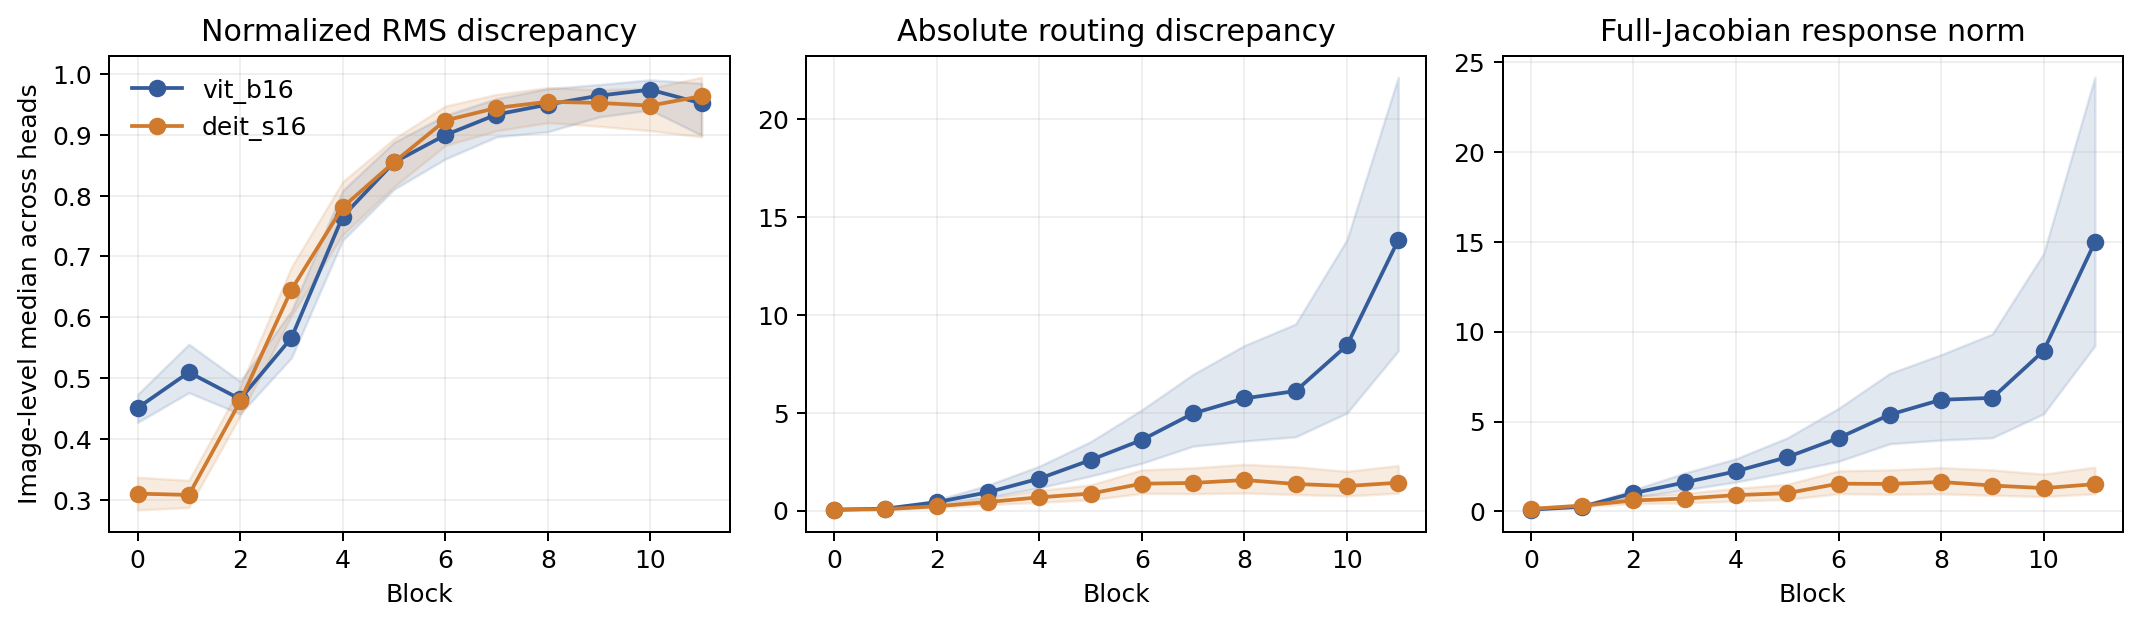
\includegraphics[keepaspectratio,alt={M4 Review Archived R2 Figure 1}]{../supplement/S77_supp_m4_review_01_m4_review_jvp_diagnostics.png}}

\textbf{M4 Review Archived R2 Figure 1.} 两模型 block 11 的 normalized
JVP discrepancy、absolute discrepancy 和 full-response denominator
分布。

控制 head projection-input activation norm 和 downstream-cotangent norm
后，两模型的 mean-query saturation 仍与 routing share、Endpoint error 和
JVP error 呈负相关。ViT-B/16 与 DeiT-S/16 的 fully adjusted correlations
依次为 −0.1442/−0.3257、 −0.1129/−0.2185 和 −0.1453/−0.2786。CLS-query
关系更弱：ViT-B 的 adjusted routing share 和 Endpoint-error 检验均为
Holm \(p=0.0629\)。因此正式 summary 使用 all-query mean
saturation，并把关联主要定位在 early/middle blocks。

\refstepcounter{figure}\label{fig:zh-supplement-002}
\pandocbounded{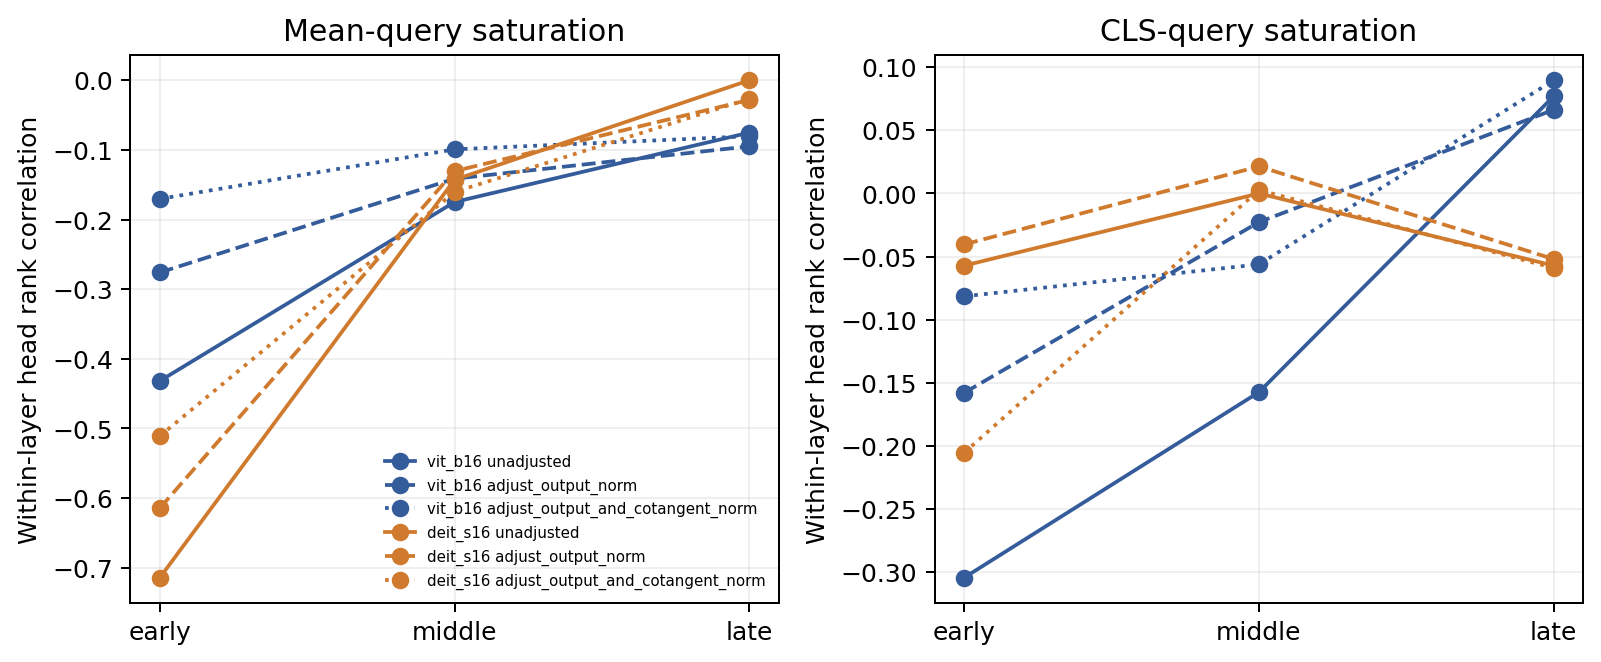
\includegraphics[keepaspectratio,alt={M4 Review Archived R2 Figure 2}]{../supplement/S78_supp_m4_review_02_m4_review_saturation_robustness.png}}

\textbf{M4 Review Archived R2 Figure 2.} Saturation 的
unadjusted/partial-rank 关系、phase sensitivity 与较弱的 CLS-query
结果。

全 cohort 空间分析使用 output 与 identity 的归一化 14×14 patch absolute
distributions 之间的 total variation。Attention residual 的
late-minus-early 差在 ViT-B/16 和 DeiT-S/16 中为 +0.0520（{[}0.0488,
0.0547{]}）和 +0.0282（{[}0.0257, 0.0300{]}）；MLP residual 为
−0.0187（{[}−0.0220, −0.0150{]}）和 −0.0462（{[}−0.0516,
−0.0412{]}）。四项 post-hoc sensitivity tests 全部通过 Holm
校正，branch-relative path scale 与 spatial TV 在图内跨层 也呈正相关。

\refstepcounter{figure}\label{fig:zh-supplement-003}
\pandocbounded{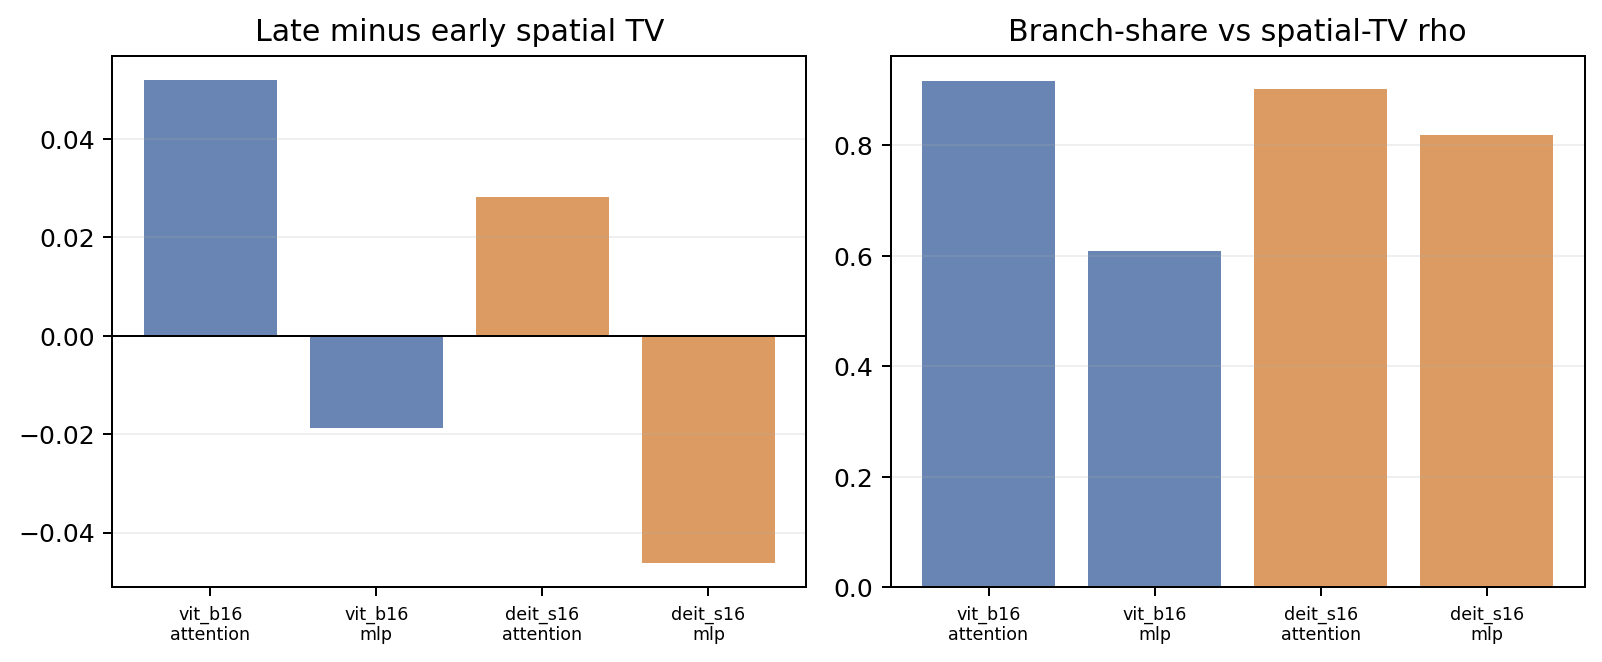
\includegraphics[keepaspectratio,alt={M4 Review Archived R2 Figure 3}]{../supplement/S79_supp_m4_review_03_m4_review_residual_spatial.png}}

\textbf{M4 Review Archived R2 Figure 3.} Attention 与 MLP 子层的全
cohort residual spatial-change sensitivity。

在每模型 16 张事前保留的 class-logit maps 上，Full--Value patch TV 从
block 0 的 0.0550/0.0307 增至 block 11 的 0.1865/0.1811。其 12-block
trajectory 与 M3 entropy、 locality 和 distance 方向相容；但 M3 使用 100
图 token-channel targets，且每模型仅一张图 重叠。因此这里只形成模型级
trajectory bridge，不构成 routing 导致空间扩展的逐单元或 因果联系。

\refstepcounter{figure}\label{fig:zh-supplement-004}
\pandocbounded{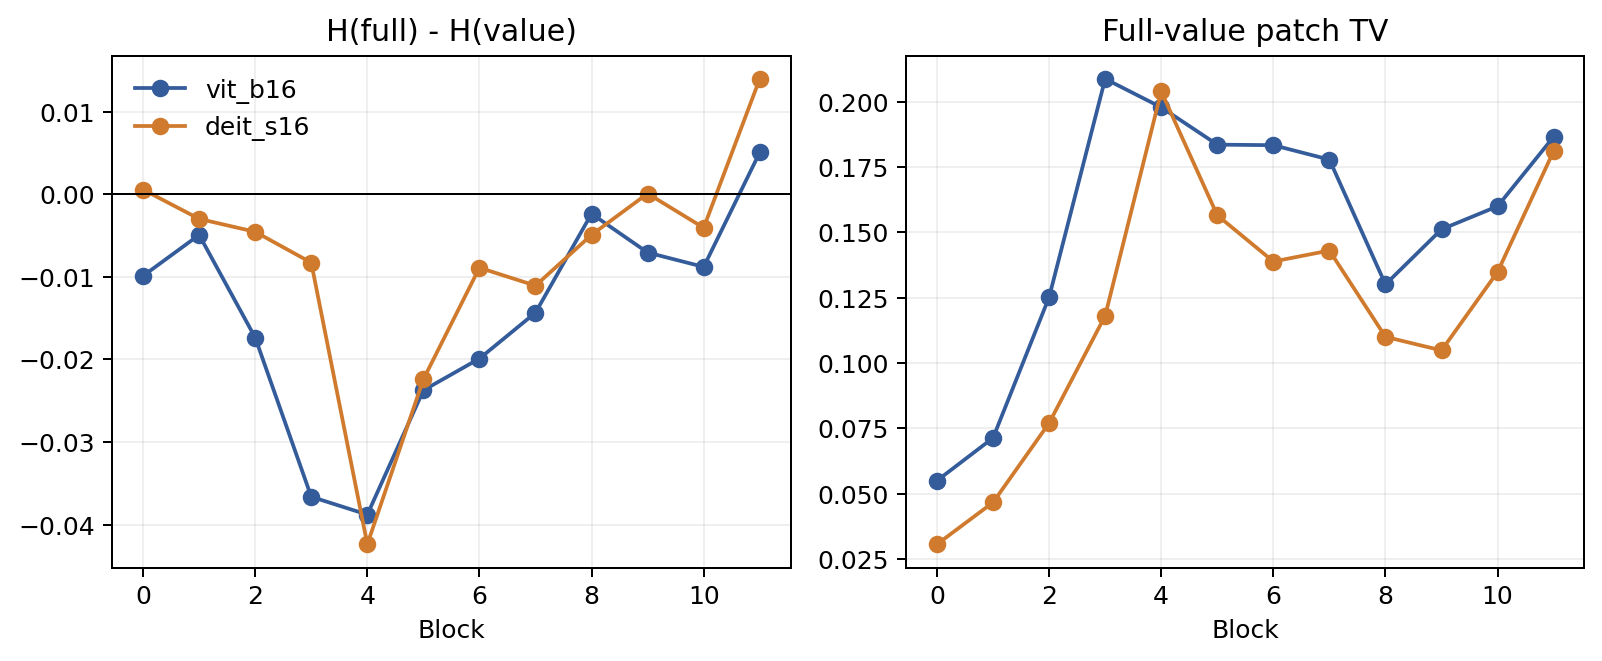
\includegraphics[keepaspectratio,alt={M4 Review Archived R2 Figure 4}]{../supplement/S80_supp_m4_review_04_m4_review_m3_m4_bridge.png}}

\textbf{M4 Review Archived R2 Figure 4.} M3 空间轨迹与 Full--Value
class-logit map 差异之间的描述性桥接。

\subsubsection{图}\label{ux56fe}

\begin{itemize}
\tightlist
\item
  Image \#1（m4\_attention\_depth）：逐 block 展示 routing
  share、frozen-attention Endpoint error 与 8-direction JVP
  error；阴影为 10,000 次图像 bootstrap 95\% CI。
\item
  Image \#2（m4\_attention\_saturation）：展示 block-level saturation 与
  routing/error 的描述性位置；正式相关检验仍使用图内 layer-wise head
  Spearman。
\item
  Image \#3（m4\_residual\_depth）：同时展示 attention/MLP residual 的
  identity share、path cancellation 和空间 TV。
\end{itemize}

\subsubsection{解释边界}\label{ux89e3ux91caux8fb9ux754c}

M4 定量描述当前输入点和冻结 ground-truth logit 下的局部 Jacobian
路径记账。较高 routing share 或 branch mass
表示该路径承载较多局部输入依赖；因果重要性仍需独立有限干预证据。

\section{S7. Complete supplementary image
index}\label{s7.-complete-supplementary-image-index}

\begin{itemize}
\tightlist
\item
  \href{../supplement/S01_figure_01_endpoint_scanner_method_overview.png}{S01
  --- S01\_figure\_01\_endpoint\_scanner\_method\_overview}
\item
  \href{../supplement/S02_figure_02_endpoint_cnn_and_path_method_identity.png}{S02
  --- S02\_figure\_02\_endpoint\_cnn\_and\_path\_method\_identity}
\item
  \href{../supplement/S03_figure_03_same_target_endpoint_versus_path.png}{S03
  --- S03\_figure\_03\_same\_target\_endpoint\_versus\_path}
\item
  \href{../supplement/S04_figure_04_original_cnn_endpoint_gates.png}{S04
  --- S04\_figure\_04\_original\_cnn\_endpoint\_gates}
\item
  \href{../supplement/S05_figure_05_attention_q_k_v_differential_paths.png}{S05
  --- S05\_figure\_05\_attention\_q\_k\_v\_differential\_paths}
\item
  \href{../supplement/S06_figure_06_residual_edge_accounting.png}{S06
  --- S06\_figure\_06\_residual\_edge\_accounting}
\item
  \href{../supplement/S07_figure_07_unit_sum_and_energy_targets.png}{S07
  --- S07\_figure\_07\_unit\_sum\_and\_energy\_targets}
\item
  \href{../supplement/S08_figure_08_state_seed_and_input_coordinates.png}{S08
  --- S08\_figure\_08\_state\_seed\_and\_input\_coordinates}
\item
  \href{../supplement/S09_figure_09_layernorm_and_gelu_jacobians.png}{S09
  --- S09\_figure\_09\_layernorm\_and\_gelu\_jacobians}
\item
  \href{../supplement/S10_figure_10_structured_edge_cuts.png}{S10 ---
  S10\_figure\_10\_structured\_edge\_cuts}
\item
  \href{../supplement/S11_figure_11_registered_target_atlas_design.png}{S11
  --- S11\_figure\_11\_registered\_target\_atlas\_design}
\item
  \href{../supplement/S12_figure_12_sloth_bear_class_logit_maps_across_models.png}{S12
  --- S12\_figure\_12\_sloth\_bear\_class\_logit\_maps\_across\_models}
\item
  \href{../supplement/S13_figure_13_sloth_bear_multi_target_atlas.png}{S13
  --- S13\_figure\_13\_sloth\_bear\_multi\_target\_atlas}
\item
  \href{../supplement/S14_figure_14_scan_scale_latency_and_resources.png}{S14
  --- S14\_figure\_14\_scan\_scale\_latency\_and\_resources}
\item
  \href{../supplement/S15_figure_15_structural_closure_contracts.png}{S15
  --- S15\_figure\_15\_structural\_closure\_contracts}
\item
  \href{../supplement/S16_figure_16_formal_closure_and_negative_controls.png}{S16
  --- S16\_figure\_16\_formal\_closure\_and\_negative\_controls}
\item
  \href{../supplement/S17_figure_17_sloth_bear_structural_component_maps.png}{S17
  --- S17\_figure\_17\_sloth\_bear\_structural\_component\_maps}
\item
  \href{../supplement/S18_figure_18_condition_scaled_analytic_jvp_checks.png}{S18
  --- S18\_figure\_18\_condition\_scaled\_analytic\_jvp\_checks}
\item
  \href{../supplement/S19_figure_19_matched_finite_activation_replacement.png}{S19
  --- S19\_figure\_19\_matched\_finite\_activation\_replacement}
\item
  \href{../supplement/S20_figure_20_c4a_family_estimates_and_intervals.png}{S20
  --- S20\_figure\_20\_c4a\_family\_estimates\_and\_intervals}
\item
  \href{../supplement/S21_figure_21_rq3_threshold_zoom_and_boundary_exception.png}{S21
  --- S21\_figure\_21\_rq3\_threshold\_zoom\_and\_boundary\_exception}
\item
  \href{../supplement/S22_figure_22_endpoint_and_registered_secondary_predictors.png}{S22
  --- S22\_figure\_22\_endpoint\_and\_registered\_secondary\_predictors}
\item
  \href{../supplement/S23_figure_23_spatial_intervention_protocol.png}{S23
  --- S23\_figure\_23\_spatial\_intervention\_protocol}
\item
  \href{../supplement/S24_figure_24_sloth_bear_block_5_maps_for_spatial_ranking.png}{S24
  ---
  S24\_figure\_24\_sloth\_bear\_block\_5\_maps\_for\_spatial\_ranking}
\item
  \href{../supplement/S25_figure_25_one_image_spatial_effect_curves.png}{S25
  --- S25\_figure\_25\_one\_image\_spatial\_effect\_curves}
\item
  \href{../supplement/S26_figure_26_c4b_mandatory_baseline_contrasts.png}{S26
  --- S26\_figure\_26\_c4b\_mandatory\_baseline\_contrasts}
\item
  \href{../supplement/S27_figure_27_rq4_family_summary.png}{S27 ---
  S27\_figure\_27\_rq4\_family\_summary}
\item
  \href{../supplement/S28_figure_28_identity_correctness_utility_conclusion.png}{S28
  --- S28\_figure\_28\_identity\_correctness\_utility\_conclusion}
\item
  \href{../supplement/S29_figure_29_m3_block_trajectories.png}{S29 ---
  S29\_figure\_29\_m3\_block\_trajectories}
\item
  \href{../supplement/S30_figure_30_m3_cls_minus_patch_entropy_by_block.png}{S30
  --- S30\_figure\_30\_m3\_cls\_minus\_patch\_entropy\_by\_block}
\item
  \href{../supplement/S31_figure_31_m3_cancellation_scales.png}{S31 ---
  S31\_figure\_31\_m3\_cancellation\_scales}
\item
  \href{../supplement/S32_figure_32_original_nns_versus_endpoint_numerical_equivalence.png}{S32
  ---
  S32\_figure\_32\_original\_nns\_versus\_endpoint\_numerical\_equivalence}
\item
  \href{../supplement/S33_figure_33_m3_finite_difference_diagnostics.png}{S33
  --- S33\_figure\_33\_m3\_finite\_difference\_diagnostics}
\item
  \href{../supplement/S34_figure_34_registered_target_learning_images.png}{S34
  --- S34\_figure\_34\_registered\_target\_learning\_images}
\item
  \href{../supplement/S35_figure_35_block5_structural_learning_images.png}{S35
  --- S35\_figure\_35\_block5\_structural\_learning\_images}
\item
  \href{../supplement/S36_figure_36_spatial_ranking_learning_images.png}{S36
  --- S36\_figure\_36\_spatial\_ranking\_learning\_images}
\item
  \href{../supplement/S37_figure_37_channel0_depth_progression.png}{S37
  --- S37\_figure\_37\_channel0\_depth\_progression}
\item
  \href{../supplement/S38_figure_38_attention_head_depth_atlas.png}{S38
  --- S38\_figure\_38\_attention\_head\_depth\_atlas}
\item
  \href{../supplement/S39_figure_39_vit_b16_attention_head_depth_atlas.png}{S39
  --- S39\_figure\_39\_vit\_b16\_attention\_head\_depth\_atlas}
\item
  \href{../supplement/S40_figure_40_vit_b16_module_chain.png}{S40 ---
  S40\_figure\_40\_vit\_b16\_module\_chain}
\item
  \href{../supplement/S41_figure_12_sloth_bear_class_logit_maps_across_models_signed.png}{S41
  ---
  S41\_figure\_12\_sloth\_bear\_class\_logit\_maps\_across\_models\_signed}
\item
  \href{../supplement/S42_figure_13_sloth_bear_multi_target_atlas_signed.png}{S42
  --- S42\_figure\_13\_sloth\_bear\_multi\_target\_atlas\_signed}
\item
  \href{../supplement/S43_figure_17_sloth_bear_structural_component_maps_signed.png}{S43
  --- S43\_figure\_17\_sloth\_bear\_structural\_component\_maps\_signed}
\item
  \href{../supplement/S44_figure_24_sloth_bear_block_5_maps_for_spatial_ranking_signed.png}{S44
  ---
  S44\_figure\_24\_sloth\_bear\_block\_5\_maps\_for\_spatial\_ranking\_signed}
\item
  \href{../supplement/S45_block_00.png}{S45 --- S45\_block\_00}
\item
  \href{../supplement/S46_block_01.png}{S46 --- S46\_block\_01}
\item
  \href{../supplement/S47_block_02.png}{S47 --- S47\_block\_02}
\item
  \href{../supplement/S48_block_03.png}{S48 --- S48\_block\_03}
\item
  \href{../supplement/S49_block_04.png}{S49 --- S49\_block\_04}
\item
  \href{../supplement/S50_block_05.png}{S50 --- S50\_block\_05}
\item
  \href{../supplement/S51_block_06.png}{S51 --- S51\_block\_06}
\item
  \href{../supplement/S52_block_07.png}{S52 --- S52\_block\_07}
\item
  \href{../supplement/S53_block_08.png}{S53 --- S53\_block\_08}
\item
  \href{../supplement/S54_block_09.png}{S54 --- S54\_block\_09}
\item
  \href{../supplement/S55_block_10.png}{S55 --- S55\_block\_10}
\item
  \href{../supplement/S56_block_11.png}{S56 --- S56\_block\_11}
\item
  \href{../supplement/S57_block_00.png}{S57 --- S57\_block\_00}
\item
  \href{../supplement/S58_block_01.png}{S58 --- S58\_block\_01}
\item
  \href{../supplement/S59_block_02.png}{S59 --- S59\_block\_02}
\item
  \href{../supplement/S60_block_03.png}{S60 --- S60\_block\_03}
\item
  \href{../supplement/S61_block_04.png}{S61 --- S61\_block\_04}
\item
  \href{../supplement/S62_block_05.png}{S62 --- S62\_block\_05}
\item
  \href{../supplement/S63_block_06.png}{S63 --- S63\_block\_06}
\item
  \href{../supplement/S64_block_07.png}{S64 --- S64\_block\_07}
\item
  \href{../supplement/S65_block_08.png}{S65 --- S65\_block\_08}
\item
  \href{../supplement/S66_block_09.png}{S66 --- S66\_block\_09}
\item
  \href{../supplement/S67_block_10.png}{S67 --- S67\_block\_10}
\item
  \href{../supplement/S68_block_11.png}{S68 --- S68\_block\_11}
\item
  \href{../supplement/S69_supp_m2_01_M2_F1.png}{S69 ---
  S69\_supp\_m2\_01\_M2\_F1}
\item
  \href{../supplement/S70_supp_m2_02_M2_F2.png}{S70 ---
  S70\_supp\_m2\_02\_M2\_F2}
\item
  \href{../supplement/S71_supp_m2_03_M2_F3.png}{S71 ---
  S71\_supp\_m2\_03\_M2\_F3}
\item
  \href{../supplement/S72_supp_m3_01_m3_atlas_depth.png}{S72 ---
  S72\_supp\_m3\_01\_m3\_atlas\_depth}
\item
  \href{../supplement/S73_supp_m3_02_m3_map_similarity.png}{S73 ---
  S73\_supp\_m3\_02\_m3\_map\_similarity}
\item
  \href{../supplement/S74_supp_m4_01_m4_attention_depth.png}{S74 ---
  S74\_supp\_m4\_01\_m4\_attention\_depth}
\item
  \href{../supplement/S75_supp_m4_02_m4_attention_saturation.png}{S75
  --- S75\_supp\_m4\_02\_m4\_attention\_saturation}
\item
  \href{../supplement/S76_supp_m4_03_m4_residual_depth.png}{S76 ---
  S76\_supp\_m4\_03\_m4\_residual\_depth}
\item
  \href{../supplement/S77_supp_m4_review_01_m4_review_jvp_diagnostics.png}{S77
  --- S77\_supp\_m4\_review\_01\_m4\_review\_jvp\_diagnostics}
\item
  \href{../supplement/S78_supp_m4_review_02_m4_review_saturation_robustness.png}{S78
  --- S78\_supp\_m4\_review\_02\_m4\_review\_saturation\_robustness}
\item
  \href{../supplement/S79_supp_m4_review_03_m4_review_residual_spatial.png}{S79
  --- S79\_supp\_m4\_review\_03\_m4\_review\_residual\_spatial}
\item
  \href{../supplement/S80_supp_m4_review_04_m4_review_m3_m4_bridge.png}{S80
  --- S80\_supp\_m4\_review\_04\_m4\_review\_m3\_m4\_bridge}
\item
  \href{../supplement/S81_supp_m6_01_m6_neuron_atlas.png}{S81 ---
  S81\_supp\_m6\_01\_m6\_neuron\_atlas}
\item
  \href{../supplement/S82_supp_m6_02_m6_model_layer_comparison.png}{S82
  --- S82\_supp\_m6\_02\_m6\_model\_layer\_comparison}
\item
  \href{../supplement/S83_supp_m6_03_m6_attention_cases.png}{S83 ---
  S83\_supp\_m6\_03\_m6\_attention\_cases}
\item
  \href{../supplement/S84_supp_m6_04_m6_residual_cases.png}{S84 ---
  S84\_supp\_m6\_04\_m6\_residual\_cases}
\item
  \href{../supplement/S85_supp_m6_05_m6_m2_semantic_boundary.png}{S85
  --- S85\_supp\_m6\_05\_m6\_m2\_semantic\_boundary}
\item
  \href{../supplement/S86_figure_34_registered_target_learning_images_signed.png}{S86
  --- S86\_figure\_34\_registered\_target\_learning\_images\_signed}
\item
  \href{../supplement/S87_figure_35_block5_structural_learning_images_signed.png}{S87
  --- S87\_figure\_35\_block5\_structural\_learning\_images\_signed}
\item
  \href{../supplement/S88_figure_36_spatial_ranking_learning_images_signed.png}{S88
  --- S88\_figure\_36\_spatial\_ranking\_learning\_images\_signed}
\item
  \href{../supplement/S89_figure_37_channel0_depth_progression_signed.png}{S89
  --- S89\_figure\_37\_channel0\_depth\_progression\_signed}
\item
  \href{../supplement/S90_figure_38_attention_head_depth_atlas_signed.png}{S90
  --- S90\_figure\_38\_attention\_head\_depth\_atlas\_signed}
\item
  \href{../supplement/S91_figure_39_vit_b16_attention_head_depth_atlas_signed.png}{S91
  --- S91\_figure\_39\_vit\_b16\_attention\_head\_depth\_atlas\_signed}
\item
  \href{../supplement/S92_figure_40_vit_b16_module_chain_signed.png}{S92
  --- S92\_figure\_40\_vit\_b16\_module\_chain\_signed}
\end{itemize}

\section{S8.
当前定性比较}\label{s8.-ux5f53ux524dux5b9aux6027ux6bd4ux8f83}

六项 CPU image-model 计算使用相同来源图像、checkpoint 与预处理。Grad-CAM
使用最后一个 norm1 的 patch activation；attention rollout 与 raw
attention
不依赖类别。展示样本不进入总体推断。具体规则见\href{../evidence/display_protocol.md}{显示协议}与\href{../evidence/compute_receipt.json}{计算收据}。

修改意见 v2 将下列展示性或重复性图件从主文移至补充材料；文件名保留原
publication-R2 编号以维持哈希和来源绑定：

\begin{itemize}
\tightlist
\item
  \href{../figures/png/fig_03_coordinate_initialization.png}{坐标初始化}
\item
  \href{../figures/png/fig_04_local_derivative_generation.png}{局部导数传播}
\item
  \href{../figures/png/fig_05_patch_embedding.png}{Patch embedding}
\item
  \href{../figures/png/fig_09_deit_s16_layerwise.png}{DeiT-S/16
  十二层图}
\item
  \href{../figures/png/fig_10_vit_b16_layerwise.png}{ViT-B/16 十二层图}
\item
  \href{../figures/png/fig_11_module_learning_images.png}{模块级学习图像与前向
  activation}
\item
  \href{../figures/png/fig_13_all_heads.png}{全部 attention heads}
\item
  \href{../figures/png/fig_14_cross_model_examples.png}{跨模型展示样本}
\item
  \href{../figures/png/fig_19_deit_s16_method_comparison.png}{DeiT-S/16
  方法展示}
\item
  \href{../figures/png/fig_20_vit_b16_method_comparison.png}{ViT-B/16
  方法展示}
\item
  \href{../figures/png/fig_22_signed_and_blue.png}{Positive、signed 与
  absolute 读图对照}
\end{itemize}

\refstepcounter{table}\label{tab:zh-supplement-008}
\textbf{Table S6. 跨 reference 排名一致性。}

{\def\LTcaptype{none} % do not increment counter
\begingroup\scriptsize
\setlength{\tabcolsep}{2pt}
\begin{longtable}[]{@{}
  >{\raggedright\arraybackslash}p{(\linewidth - 12\tabcolsep) * \real{0.1429}}
  >{\raggedright\arraybackslash}p{(\linewidth - 12\tabcolsep) * \real{0.1429}}
  >{\raggedright\arraybackslash}p{(\linewidth - 12\tabcolsep) * \real{0.1429}}
  >{\raggedright\arraybackslash}p{(\linewidth - 12\tabcolsep) * \real{0.1429}}
  >{\raggedright\arraybackslash}p{(\linewidth - 12\tabcolsep) * \real{0.1429}}
  >{\raggedright\arraybackslash}p{(\linewidth - 12\tabcolsep) * \real{0.1429}}
  >{\raggedright\arraybackslash}p{(\linewidth - 12\tabcolsep) * \real{0.1429}}@{}}
\toprule\noalign{}
\begin{minipage}[b]{\linewidth}\raggedright
Model
\end{minipage} & \begin{minipage}[b]{\linewidth}\raggedright
Quantity
\end{minipage} & \begin{minipage}[b]{\linewidth}\raggedright
Spearman
\end{minipage} & \begin{minipage}[b]{\linewidth}\raggedright
Kendall tau-b
\end{minipage} & \begin{minipage}[b]{\linewidth}\raggedright
Top-1 agreement
\end{minipage} & \begin{minipage}[b]{\linewidth}\raggedright
Top-3 overlap
\end{minipage} & \begin{minipage}[b]{\linewidth}\raggedright
Mean abs rank displacement
\end{minipage} \\
\midrule\noalign{}
\endhead
\bottomrule\noalign{}
\endlastfoot
DeiT-S/16 & finite\_effect & 0.3071 & 0.2444 & 0.4167 & 0.6111 &
1.5278 \\
DeiT-S/16 & taylor & 0.3000 & 0.2389 & 0.3333 & 0.6111 & 1.5278 \\
ViT-B/16 & finite\_effect & 0.3759 & 0.2803 & 0.3333 & 0.5000 &
2.9444 \\
ViT-B/16 & taylor & 0.3782 & 0.2828 & 0.3333 & 0.5000 & 2.9444 \\
\end{longtable}
\endgroup
}

\href{supplement_experiments_v1.md}{新增补充实验 S9--S14}

本补充完成建议文档第十一节的最低实验包与两项 P0
修正。新增结果为补充描述性分析；原确认性决策及封存证据保留。所有实验先冻结
cohort、通道、初始化种子和统计规则，再运行模型。

\section{S9.
随机区域基线修正}\label{s9.-ux968fux673aux533aux57dfux57faux7ebfux4feeux6b63}

每个随机重复先对效应取绝对值并计算 AUC，再平均 20 次重复及图内
heads。旧估计器先平均 signed curves，因正负抵消低估 absolute-effect
random baseline。下表比较 400 图 family
的图像级中位数及配对中位差；区间为 2,000 次图像 bootstrap。

\begin{equation}\label{eq:zh-supplement-001}
\widehat A_{\rm random}=\frac1R\sum_{r=1}^R\frac1{0.25}\int_0^{0.25}|e_r(a)|\,da.
\end{equation}

{\def\LTcaptype{none} % do not increment counter
\begingroup\scriptsize
\setlength{\tabcolsep}{2pt}
\begin{longtable}[]{@{}
  >{\raggedright\arraybackslash}p{(\linewidth - 12\tabcolsep) * \real{0.1429}}
  >{\raggedright\arraybackslash}p{(\linewidth - 12\tabcolsep) * \real{0.1429}}
  >{\raggedright\arraybackslash}p{(\linewidth - 12\tabcolsep) * \real{0.1429}}
  >{\raggedright\arraybackslash}p{(\linewidth - 12\tabcolsep) * \real{0.1429}}
  >{\raggedright\arraybackslash}p{(\linewidth - 12\tabcolsep) * \real{0.1429}}
  >{\raggedright\arraybackslash}p{(\linewidth - 12\tabcolsep) * \real{0.1429}}
  >{\raggedright\arraybackslash}p{(\linewidth - 12\tabcolsep) * \real{0.1429}}@{}}
\toprule\noalign{}
\begin{minipage}[b]{\linewidth}\raggedright
Model
\end{minipage} & \begin{minipage}[b]{\linewidth}\raggedright
Reference
\end{minipage} & \begin{minipage}[b]{\linewidth}\raggedright
Legacy random median
\end{minipage} & \begin{minipage}[b]{\linewidth}\raggedright
Corrected random mean
\end{minipage} & \begin{minipage}[b]{\linewidth}\raggedright
Corrected random median
\end{minipage} & \begin{minipage}[b]{\linewidth}\raggedright
Endpoint - random median {[}95\% CI{]}
\end{minipage} & \begin{minipage}[b]{\linewidth}\raggedright
Taylor - random median {[}95\% CI{]}
\end{minipage} \\
\midrule\noalign{}
\endhead
\bottomrule\noalign{}
\endlastfoot
ViT-B/16 & normalized-zero & 0.0294 & 0.0366 & 0.0339 & -0.0023
{[}-0.0033, -0.0015{]} & 0.0207 {[}0.0192, 0.0221{]} \\
ViT-B/16 & blur & 0.0225 & 0.0355 & 0.0307 & -0.0031 {[}-0.0045,
-0.0016{]} & 0.0219 {[}0.0197, 0.0232{]} \\
DeiT-S/16 & normalized-zero & 0.0475 & 0.0728 & 0.0611 & 0.0009
{[}-0.0009, 0.0029{]} & 0.0329 {[}0.0289, 0.0365{]} \\
DeiT-S/16 & blur & 0.0296 & 0.0505 & 0.0411 & -0.0010 {[}-0.0025,
0.0007{]} & 0.0336 {[}0.0311, 0.0371{]} \\
\end{longtable}
\endgroup
}

修正后 ViT-B 两种 reference 的 Endpoint−random 中位差均为负；DeiT-S
的两个区间跨零。Taylor−random 四个区间均为正。Endpoint−Taylor
比较保持不变。

\refstepcounter{figure}\label{fig:zh-supplement-005}
\pandocbounded{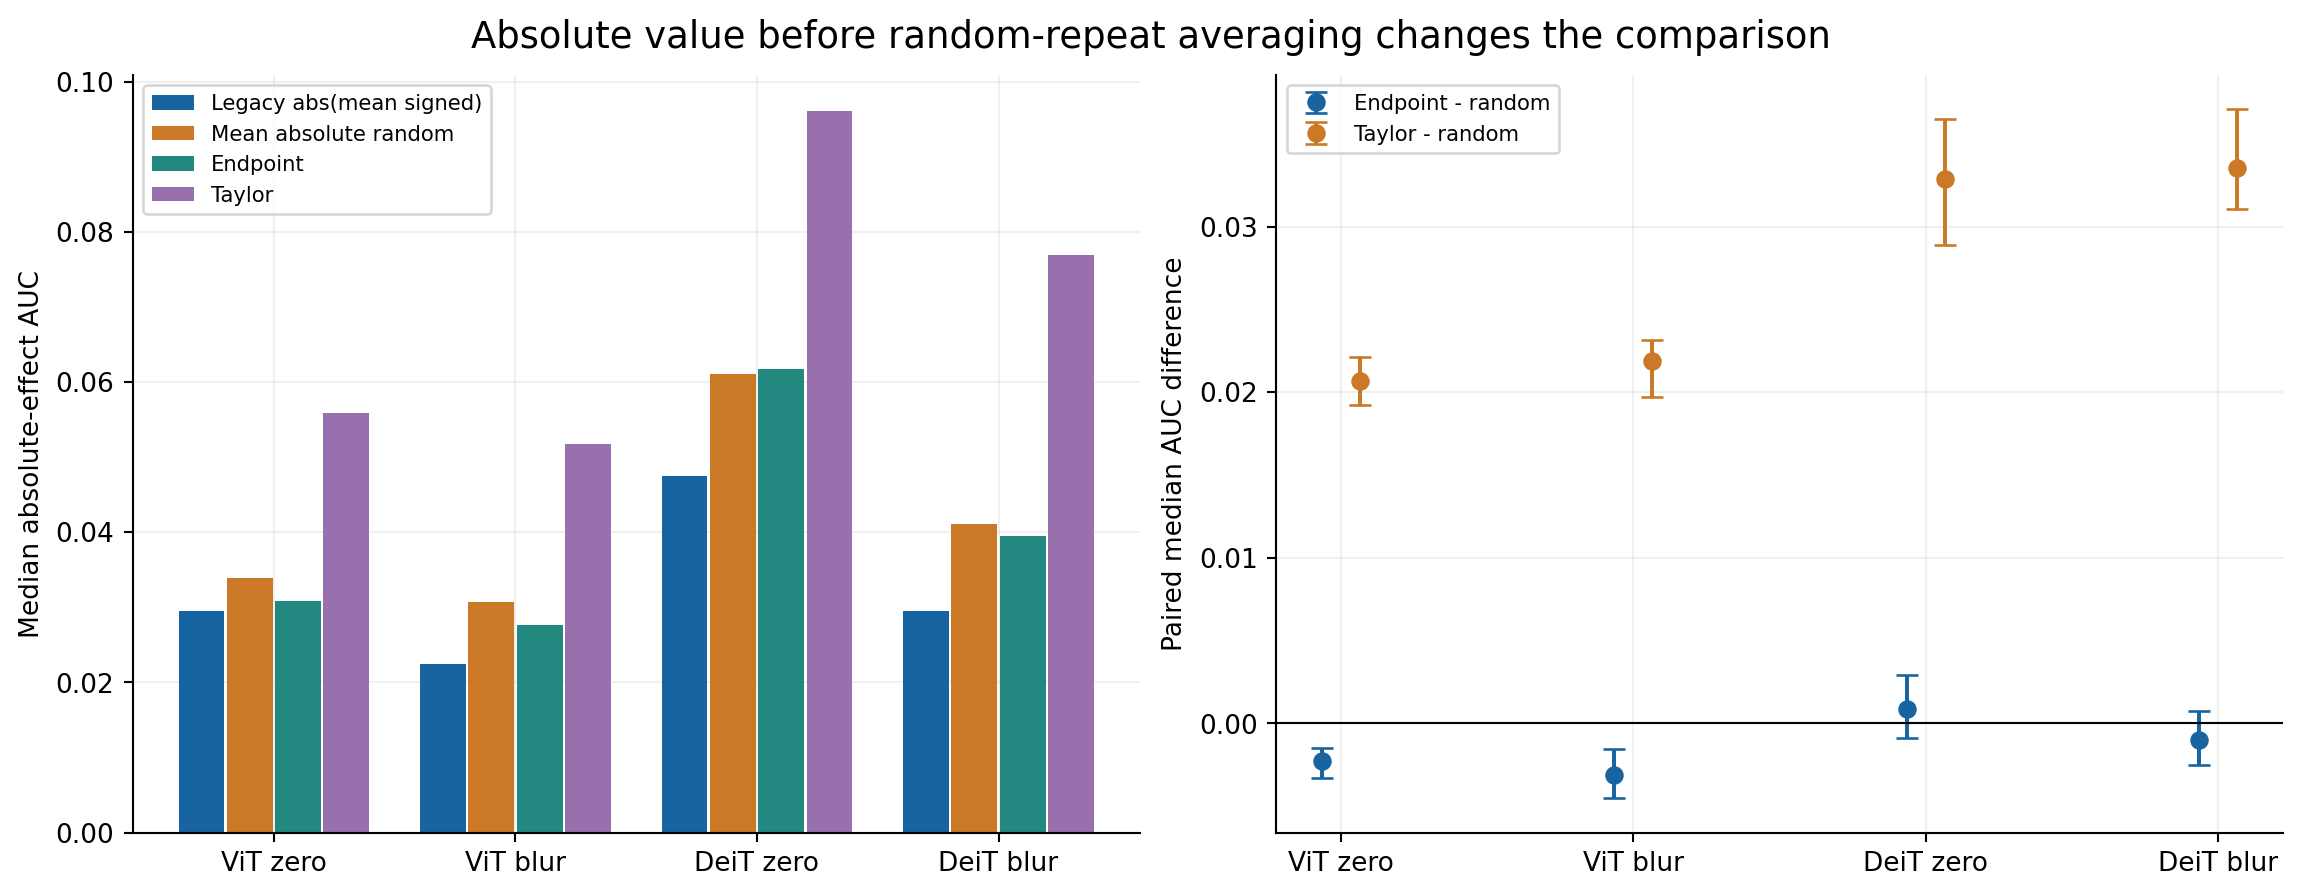
\includegraphics[keepaspectratio,alt={Supplement Figure 1}]{../evidence/supplement_v1/sup_01_random_correction.png}}

每图随机均值的相对 MC 标准误中位数为 5.1\%--6.9\%，q90 为
7.6\%--8.9\%。从现有 20 次重复进行 5/10/20
次有放回重采样，误差随重复数减少而增大。固定图像下 cohort mean 的 Monte
Carlo
误差小于图像抽样不确定性；单图细小优势仍不适合据此判定。该诊断只覆盖已观察的随机重复，不能证明任意精度下
20 次都足够。

{\def\LTcaptype{none} % do not increment counter
\begingroup\scriptsize
\setlength{\tabcolsep}{2pt}
\begin{longtable}[]{@{}
  >{\raggedright\arraybackslash}p{(\linewidth - 12\tabcolsep) * \real{0.1429}}
  >{\raggedright\arraybackslash}p{(\linewidth - 12\tabcolsep) * \real{0.1429}}
  >{\raggedright\arraybackslash}p{(\linewidth - 12\tabcolsep) * \real{0.1429}}
  >{\raggedright\arraybackslash}p{(\linewidth - 12\tabcolsep) * \real{0.1429}}
  >{\raggedright\arraybackslash}p{(\linewidth - 12\tabcolsep) * \real{0.1429}}
  >{\raggedright\arraybackslash}p{(\linewidth - 12\tabcolsep) * \real{0.1429}}
  >{\raggedright\arraybackslash}p{(\linewidth - 12\tabcolsep) * \real{0.1429}}@{}}
\toprule\noalign{}
\begin{minipage}[b]{\linewidth}\raggedright
Model
\end{minipage} & \begin{minipage}[b]{\linewidth}\raggedright
Reference
\end{minipage} & \begin{minipage}[b]{\linewidth}\raggedright
Median relative MC SE
\end{minipage} & \begin{minipage}[b]{\linewidth}\raggedright
q90 relative MC SE
\end{minipage} & \begin{minipage}[b]{\linewidth}\raggedright
MC image error R=5
\end{minipage} & \begin{minipage}[b]{\linewidth}\raggedright
R=10
\end{minipage} & \begin{minipage}[b]{\linewidth}\raggedright
R=20
\end{minipage} \\
\midrule\noalign{}
\endhead
\bottomrule\noalign{}
\endlastfoot
ViT-B/16 & normalized-zero & 0.0506 & 0.0759 & 0.0020 & 0.0014 &
0.0010 \\
ViT-B/16 & blur & 0.0665 & 0.0883 & 0.0026 & 0.0018 & 0.0013 \\
DeiT-S/16 & normalized-zero & 0.0622 & 0.0851 & 0.0046 & 0.0032 &
0.0023 \\
DeiT-S/16 & blur & 0.0687 & 0.0895 & 0.0035 & 0.0024 & 0.0017 \\
\end{longtable}
\endgroup
}

\href{../evidence/supplement_v1/baseline_repeat_cohort_values.csv}{20-repeat
cohort distribution} ·
\href{../evidence/supplement_v1/baseline_repeat_image_values.csv}{Per-image
repeats} ·
\href{../evidence/supplement_v1/baseline_image_values.csv}{Paired image
values, MC SE, split-half and leave-one-repeat-out}

\section{S10.
训练与随机初始化}\label{s10.-ux8badux7ec3ux4e0eux968fux673aux521dux59cbux5316}

ViT-B/16 和 DeiT-S/16 各使用 3
个随机初始化状态（202609201、202609202、202609203），与训练模型共享原 M3
cohort 的前 32 图、全部 12 blocks、16 tokens 和每层 16 个冻结
channels，M4 覆盖全部 heads。随机模型采用相同 timm 0.9.16
架构与默认初始化；同一状态用于全部图像。训练结果由同图、同目标的原始
M3/M4
数组筛选得到。图内先聚合，early=0--3、late=8--11；训练−随机区间同时重采样共享图像和模型种子（2,000
次），保留种子层级。

随机模型已出现 entropy 增大、locality
减小及距离增大，表明空间扩展并非训练参数状态独有。训练模型的 entropy
late−early 为 0.2288/0.2256，随机参数状态均值为
0.0940/0.1718；两种参数状态的扩展幅度存在差异。训练参数状态的 routing
scale 增大，而随机参数状态均值为负；attention identity
的层深趋势也在两种参数状态间反向。MLP identity 在两类状态中均增加，ViT-B
的训练参数状态减随机参数状态区间包含零。三个随机状态限制了对初始化总体的推断；该对照不识别训练过程的因果效应，也不单独识别架构与初始化的贡献。

{\def\LTcaptype{none} % do not increment counter
\begingroup\scriptsize
\setlength{\tabcolsep}{2pt}
\begin{longtable}[]{@{}
  >{\raggedright\arraybackslash}p{(\linewidth - 12\tabcolsep) * \real{0.1429}}
  >{\raggedright\arraybackslash}p{(\linewidth - 12\tabcolsep) * \real{0.1429}}
  >{\raggedright\arraybackslash}p{(\linewidth - 12\tabcolsep) * \real{0.1429}}
  >{\raggedright\arraybackslash}p{(\linewidth - 12\tabcolsep) * \real{0.1429}}
  >{\raggedright\arraybackslash}p{(\linewidth - 12\tabcolsep) * \real{0.1429}}
  >{\raggedright\arraybackslash}p{(\linewidth - 12\tabcolsep) * \real{0.1429}}
  >{\raggedright\arraybackslash}p{(\linewidth - 12\tabcolsep) * \real{0.1429}}@{}}
\toprule\noalign{}
\begin{minipage}[b]{\linewidth}\raggedright
Model
\end{minipage} & \begin{minipage}[b]{\linewidth}\raggedright
Study
\end{minipage} & \begin{minipage}[b]{\linewidth}\raggedright
Metric
\end{minipage} & \begin{minipage}[b]{\linewidth}\raggedright
Trained late - early
\end{minipage} & \begin{minipage}[b]{\linewidth}\raggedright
Random late - early
\end{minipage} & \begin{minipage}[b]{\linewidth}\raggedright
Trained - random {[}95\% CI{]}
\end{minipage} & \begin{minipage}[b]{\linewidth}\raggedright
Random seed 1 / 2 / 3
\end{minipage} \\
\midrule\noalign{}
\endhead
\bottomrule\noalign{}
\endlastfoot
DeiT-S/16 & m3 & cancellation & 0.0020 & 0.0036 & -0.0016 {[}-0.0029,
-0.0005{]} & 0.0032 / 0.0028 / 0.0050 \\
DeiT-S/16 & m3 & cls\_minus\_patch\_entropy & -0.2685 & -0.1717 &
-0.0968 {[}-0.1051, -0.0889{]} & -0.1697 / -0.1740 / -0.1714 \\
DeiT-S/16 & m3 & distance & 0.1276 & 0.0576 & 0.0700 {[}0.0624,
0.0781{]} & 0.0574 / 0.0584 / 0.0569 \\
DeiT-S/16 & m3 & entropy & 0.2256 & 0.1718 & 0.0539 {[}0.0473, 0.0602{]}
& 0.1699 / 0.1740 / 0.1714 \\
DeiT-S/16 & m3 & locality & -0.3441 & -0.1445 & -0.1997 {[}-0.2115,
-0.1882{]} & -0.1433 / -0.1466 / -0.1436 \\
DeiT-S/16 & m4 & attention\_identity\_scale & -0.0579 & 0.1188 & -0.1767
{[}-0.1916, -0.1618{]} & 0.1232 / 0.1142 / 0.1190 \\
DeiT-S/16 & m4 & attention\_output\_identity\_tv & 0.0306 & -0.0026 &
0.0331 {[}0.0274, 0.0388{]} & -0.0029 / -0.0025 / -0.0023 \\
DeiT-S/16 & m4 & attention\_path\_cancellation & 0.0958 & -0.0042 &
0.1001 {[}0.0890, 0.1115{]} & 0.0002 / -0.0036 / -0.0093 \\
DeiT-S/16 & m4 & attention\_residual\_path\_cancellation & 0.0188 &
-0.0848 & 0.1036 {[}0.0810, 0.1271{]} & -0.0889 / -0.0770 / -0.0884 \\
DeiT-S/16 & m4 & jvp\_discrepancy & 0.5465 & -0.0944 & 0.6409 {[}0.6150,
0.6673{]} & -0.0871 / -0.0859 / -0.1101 \\
DeiT-S/16 & m4 & mlp\_identity\_scale & 0.2063 & 0.1461 & 0.0602
{[}0.0308, 0.0907{]} & 0.1423 / 0.1431 / 0.1528 \\
DeiT-S/16 & m4 & mlp\_output\_identity\_tv & -0.0610 & -0.0041 & -0.0569
{[}-0.0722, -0.0413{]} & -0.0047 / -0.0042 / -0.0034 \\
DeiT-S/16 & m4 & mlp\_residual\_path\_cancellation & -0.0381 & -0.0756 &
0.0375 {[}0.0101, 0.0675{]} & -0.0731 / -0.0761 / -0.0775 \\
DeiT-S/16 & m4 & routing\_scale & 0.1314 & -0.0043 & 0.1357 {[}0.1151,
0.1564{]} & 0.0023 / -0.0032 / -0.0120 \\
DeiT-S/16 & m4 & saturation\_error & 0.7536 & -0.0348 & 0.7884
{[}0.6387, 0.9354{]} & -0.0348 / -0.0348 / -0.0348 \\
DeiT-S/16 & m4 & saturation\_routing & 0.7598 & -0.0348 & 0.7946
{[}0.6417, 0.9491{]} & -0.0357 / -0.0339 / -0.0348 \\
DeiT-S/16 & m4 & value\_error & 0.2676 & -0.0088 & 0.2764 {[}0.2406,
0.3122{]} & -0.0008 / -0.0071 / -0.0184 \\
ViT-B/16 & m3 & cancellation & 0.0024 & 0.0008 & 0.0016 {[}0.0008,
0.0023{]} & 0.0014 / 0.0010 / 0.0000 \\
ViT-B/16 & m3 & cls\_minus\_patch\_entropy & -0.2741 & -0.0940 & -0.1802
{[}-0.1893, -0.1709{]} & -0.0933 / -0.0970 / -0.0917 \\
ViT-B/16 & m3 & distance & 0.1292 & 0.0399 & 0.0893 {[}0.0833, 0.0953{]}
& 0.0399 / 0.0410 / 0.0387 \\
ViT-B/16 & m3 & entropy & 0.2288 & 0.0940 & 0.1348 {[}0.1232, 0.1466{]}
& 0.0934 / 0.0968 / 0.0918 \\
ViT-B/16 & m3 & locality & -0.3522 & -0.1005 & -0.2517 {[}-0.2598,
-0.2431{]} & -0.1001 / -0.1036 / -0.0979 \\
ViT-B/16 & m4 & attention\_identity\_scale & -0.1144 & 0.1631 & -0.2775
{[}-0.3004, -0.2520{]} & 0.1629 / 0.1662 / 0.1603 \\
ViT-B/16 & m4 & attention\_output\_identity\_tv & 0.0507 & -0.0046 &
0.0553 {[}0.0454, 0.0644{]} & -0.0042 / -0.0040 / -0.0058 \\
ViT-B/16 & m4 & attention\_path\_cancellation & 0.0797 & -0.0421 &
0.1218 {[}0.1136, 0.1303{]} & -0.0428 / -0.0413 / -0.0423 \\
ViT-B/16 & m4 & attention\_residual\_path\_cancellation & 0.0138 &
-0.1050 & 0.1188 {[}0.0932, 0.1447{]} & -0.1028 / -0.1084 / -0.1038 \\
ViT-B/16 & m4 & jvp\_discrepancy & 0.4501 & -0.2600 & 0.7101 {[}0.6739,
0.7465{]} & -0.2621 / -0.2548 / -0.2631 \\
ViT-B/16 & m4 & mlp\_identity\_scale & 0.1951 & 0.1819 & 0.0132
{[}-0.0093, 0.0361{]} & 0.1829 / 0.1851 / 0.1775 \\
ViT-B/16 & m4 & mlp\_output\_identity\_tv & -0.0205 & -0.0042 & -0.0163
{[}-0.0295, -0.0047{]} & -0.0041 / -0.0045 / -0.0041 \\
ViT-B/16 & m4 & mlp\_residual\_path\_cancellation & 0.0887 & -0.0866 &
0.1753 {[}0.1350, 0.2174{]} & -0.0845 / -0.0907 / -0.0846 \\
ViT-B/16 & m4 & routing\_scale & 0.0512 & -0.0479 & 0.0991 {[}0.0810,
0.1160{]} & -0.0485 / -0.0470 / -0.0481 \\
ViT-B/16 & m4 & saturation\_error & 0.3568 & 0.0232 & 0.3336 {[}0.2370,
0.4496{]} & 0.0827 / -0.0498 / 0.0366 \\
ViT-B/16 & m4 & saturation\_routing & 0.4379 & 0.0203 & 0.4177
{[}0.3136, 0.5211{]} & 0.0636 / -0.0431 / 0.0402 \\
ViT-B/16 & m4 & value\_error & 0.1437 & -0.0623 & 0.2061 {[}0.1689,
0.2420{]} & -0.0621 / -0.0615 / -0.0633 \\
\end{longtable}
\endgroup
}

\refstepcounter{figure}\label{fig:zh-supplement-006}
\pandocbounded{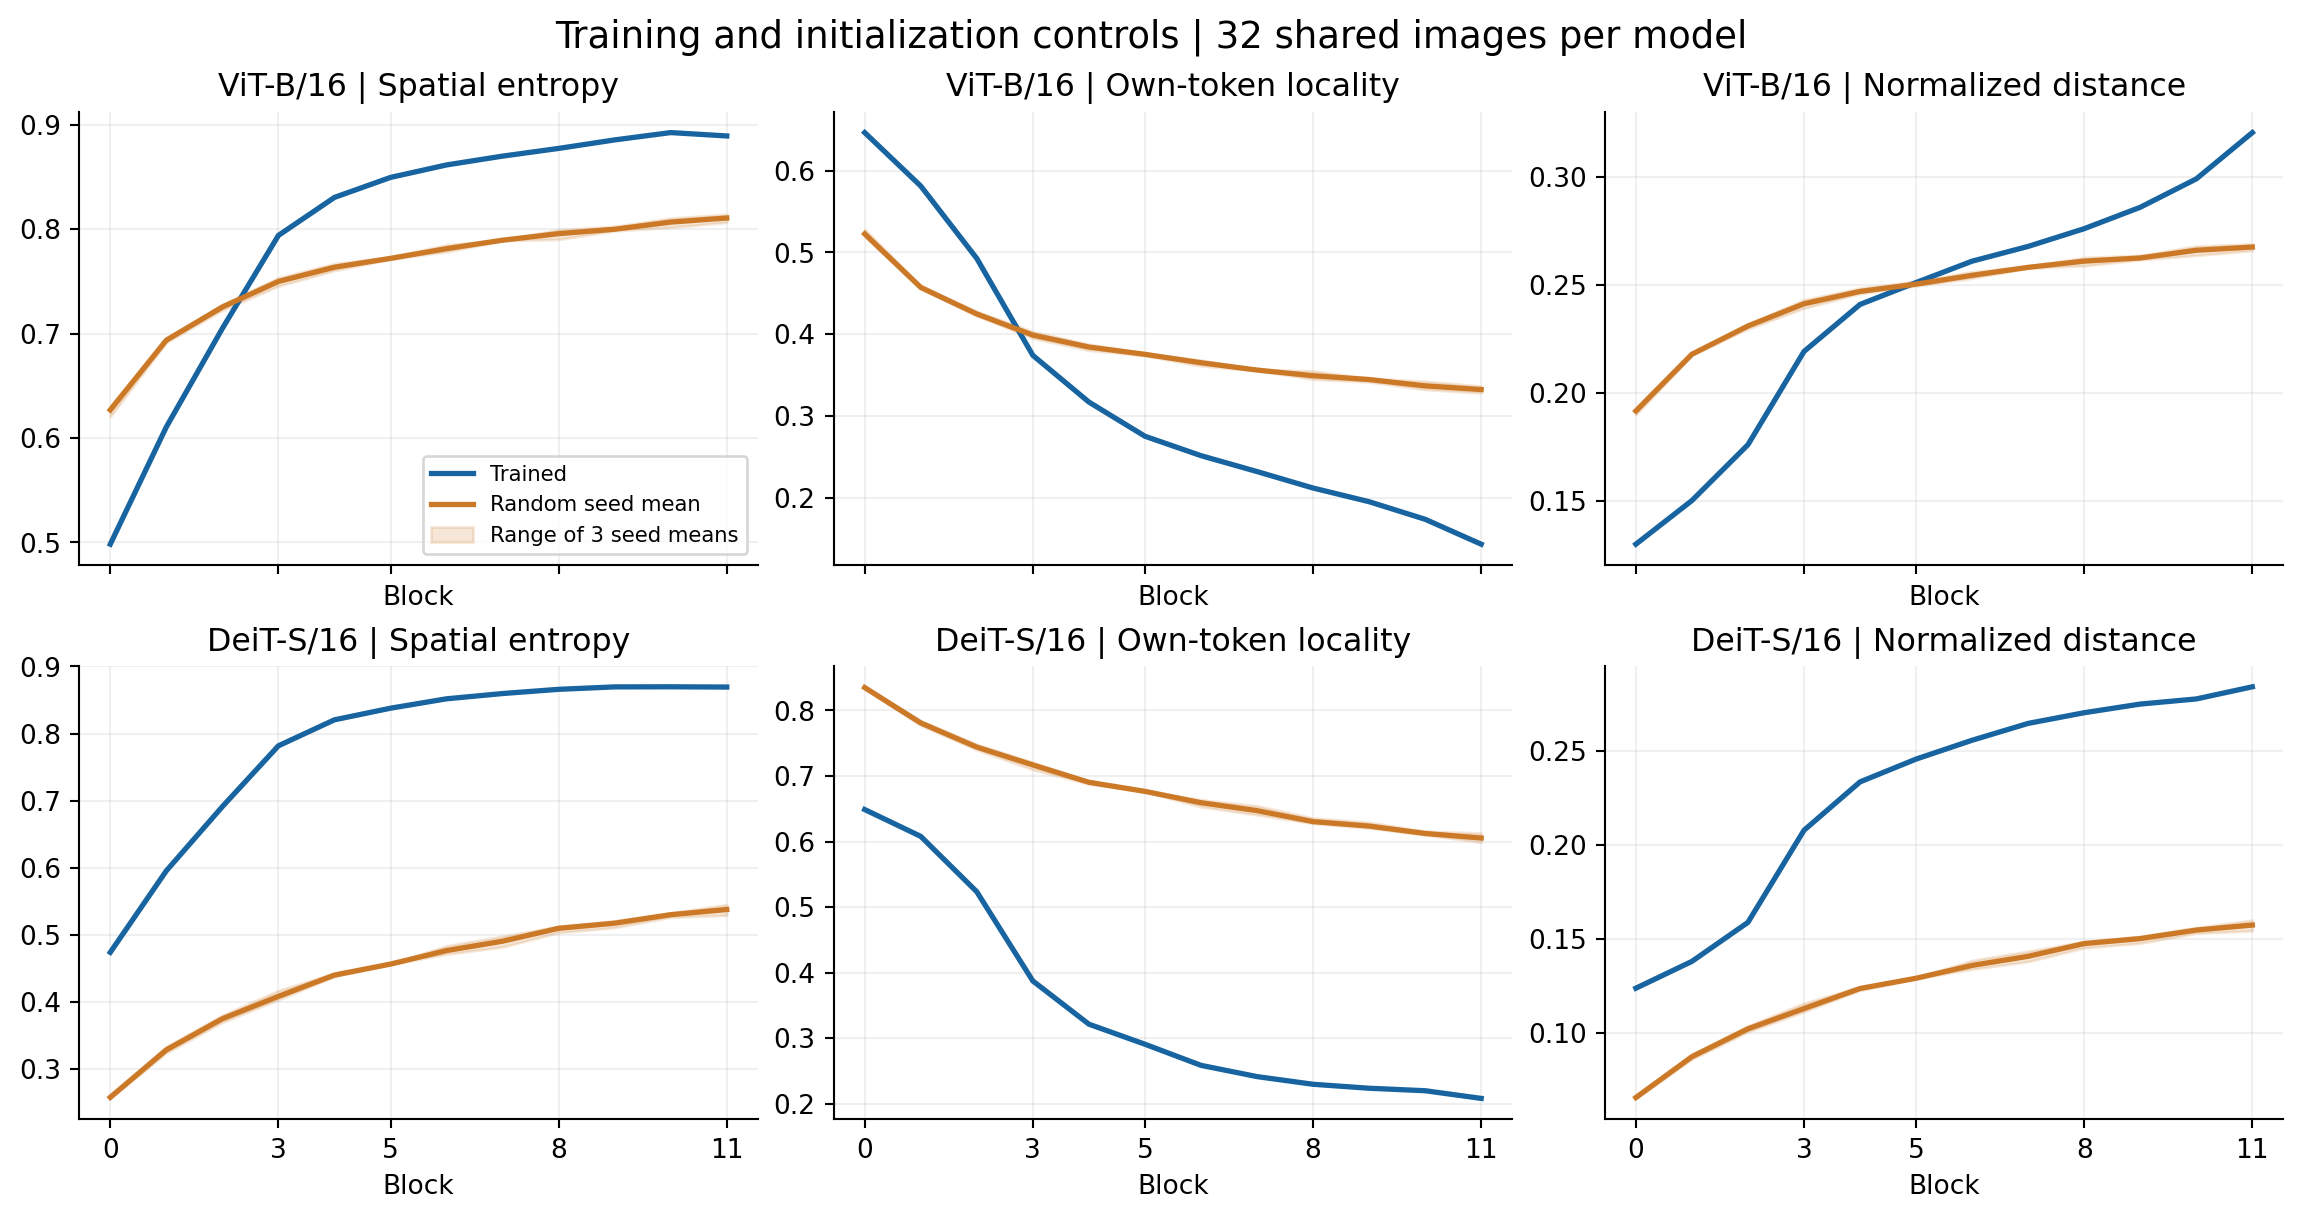
\includegraphics[keepaspectratio,alt={Supplement Figure 2}]{../evidence/supplement_v1/sup_02_m3_training.png}}

\refstepcounter{figure}\label{fig:zh-supplement-007}
\pandocbounded{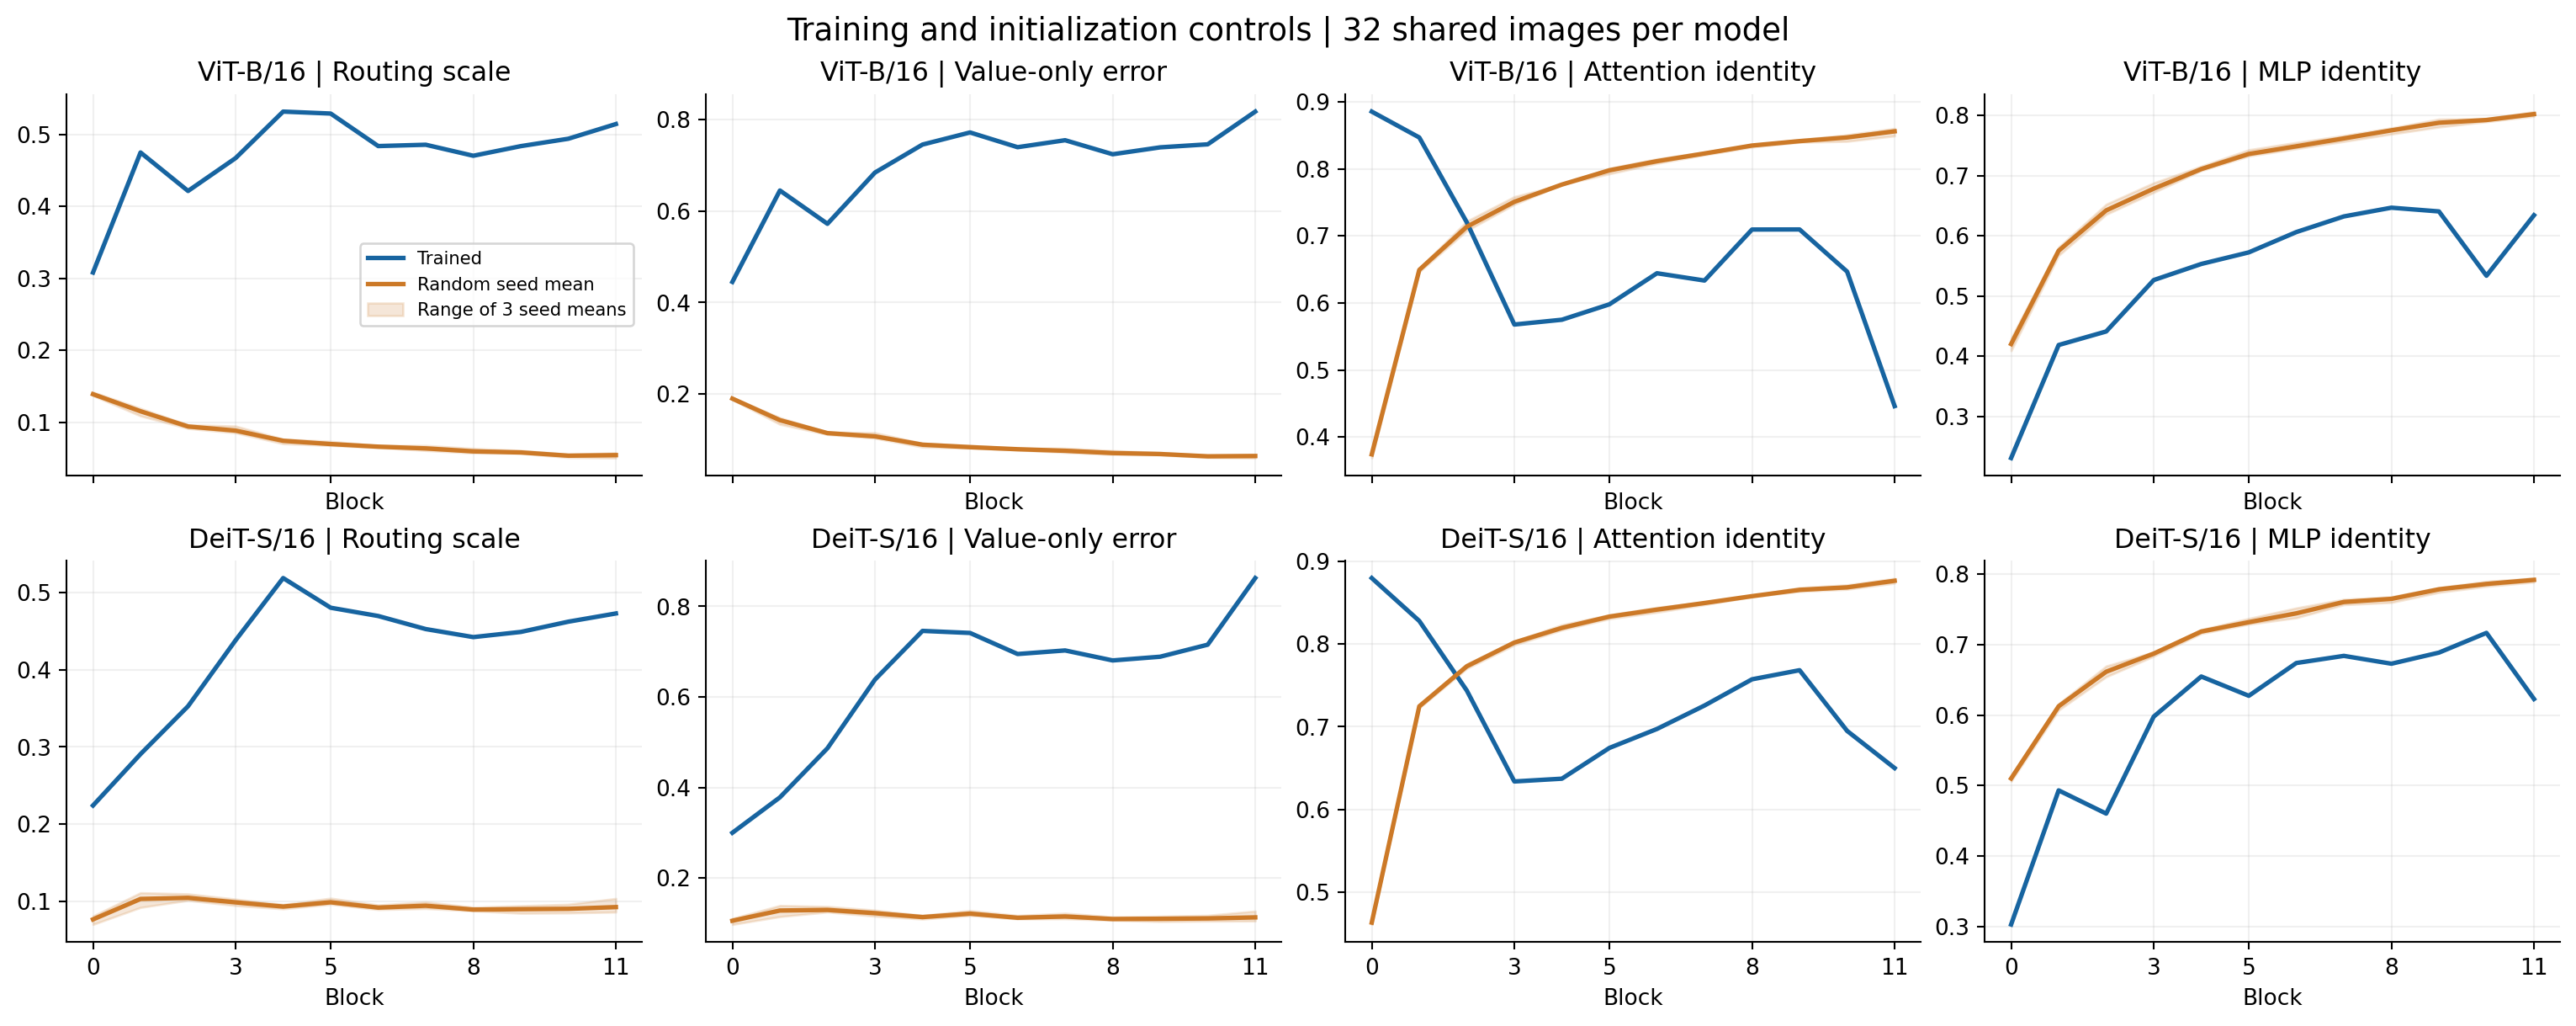
\includegraphics[keepaspectratio,alt={Supplement Figure 3}]{../evidence/supplement_v1/sup_03_m4_training.png}}

\href{../evidence/supplement_v1/training_analysis.json}{Early/late and
difference estimates} ·
\href{../evidence/supplement_v1/training_image_trends.csv}{Image values}

\section{S11. 目标稳健性}\label{s11.-ux76eeux6807ux7a33ux5065ux6027}

原 M3 冻结 100 图/模型，GT、clean-top1、top1−runnerup 三目标，blocks
0/5/11、全部 heads。分类索引固定于 clean 输入。正确/错误图分别为 ViT-B
92/8、DeiT-S 86/14；正确图的 GT 与 top1 完全一致。下表报告每图 head
聚合后的 B11−B0，并按 all/correct/incorrect
分组；所有目标在同一组使用相同 bootstrap 图像索引。

routing scale 和 Value-only error 在三种目标中均随深度增加；attention
identity 减少，MLP identity 增加，正确与错误子集方向一致。Margin
改变幅度，例如 ViT-B routing 增量由 GT 的 0.2031 降至 0.1439，DeiT-S
attention identity 降幅由 −0.2168 变为 −0.1014。两模型错误子集只有 8/14
图，其区间相应反映较少的图像信息。

native attention-output JVP 只依赖模型与输入，不依赖被解释的类别；其 8
方向 discrepancy 从原 M4 同图记录继承。target\_contracted\_jvp
另用每个目标对 head 输出的 cotangent 收缩方向导数，衡量目标相关
Value-only discrepancy。两者作为不同指标报告。Saturation relation
为图内同 block 跨 head 的 Spearman，并报告其层深变化；完整 block
值、目标配对差和 NA 数量见数据文件。

\refstepcounter{figure}\label{fig:zh-supplement-008}
\pandocbounded{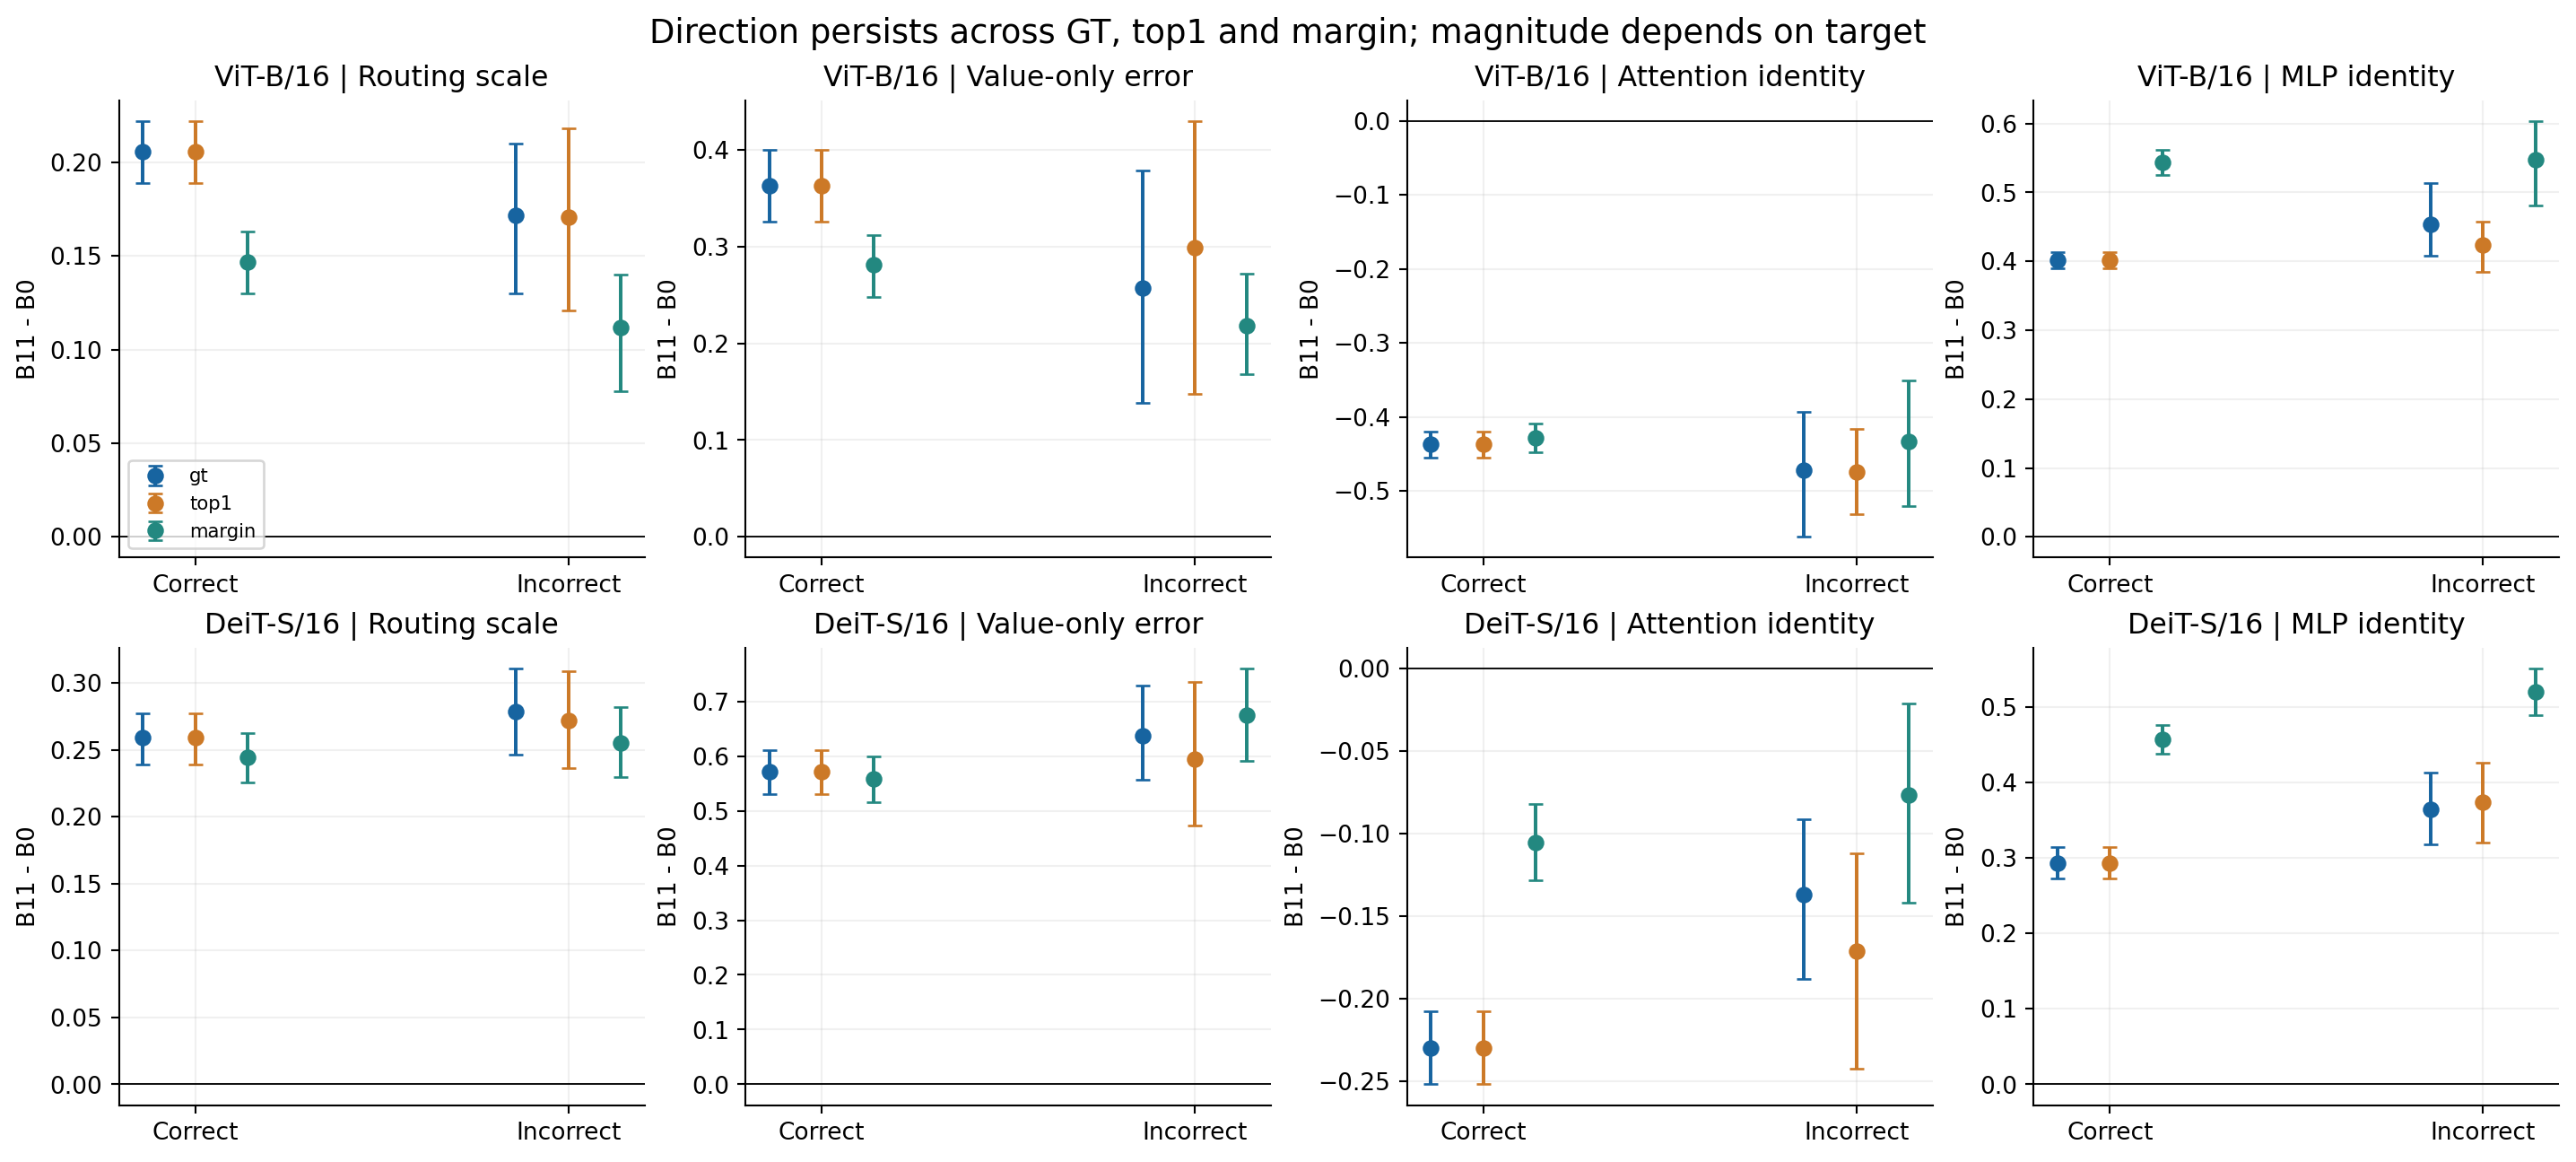
\includegraphics[keepaspectratio,alt={Supplement Figure 4}]{../evidence/supplement_v1/sup_04_target_robustness.png}}

{\def\LTcaptype{none} % do not increment counter
\begingroup\scriptsize
\setlength{\tabcolsep}{2pt}
\begin{longtable}[]{@{}
  >{\raggedright\arraybackslash}p{(\linewidth - 12\tabcolsep) * \real{0.1429}}
  >{\raggedright\arraybackslash}p{(\linewidth - 12\tabcolsep) * \real{0.1429}}
  >{\raggedright\arraybackslash}p{(\linewidth - 12\tabcolsep) * \real{0.1429}}
  >{\raggedright\arraybackslash}p{(\linewidth - 12\tabcolsep) * \real{0.1429}}
  >{\raggedright\arraybackslash}p{(\linewidth - 12\tabcolsep) * \real{0.1429}}
  >{\raggedright\arraybackslash}p{(\linewidth - 12\tabcolsep) * \real{0.1429}}
  >{\raggedright\arraybackslash}p{(\linewidth - 12\tabcolsep) * \real{0.1429}}@{}}
\toprule\noalign{}
\begin{minipage}[b]{\linewidth}\raggedright
Model
\end{minipage} & \begin{minipage}[b]{\linewidth}\raggedright
Subset
\end{minipage} & \begin{minipage}[b]{\linewidth}\raggedright
Target
\end{minipage} & \begin{minipage}[b]{\linewidth}\raggedright
Metric
\end{minipage} & \begin{minipage}[b]{\linewidth}\raggedright
n
\end{minipage} & \begin{minipage}[b]{\linewidth}\raggedright
B11 - B0 mean
\end{minipage} & \begin{minipage}[b]{\linewidth}\raggedright
95\% CI
\end{minipage} \\
\midrule\noalign{}
\endhead
\bottomrule\noalign{}
\endlastfoot
ViT-B/16 & all & gt & routing\_scale & 100 & 0.2031 & {[}0.1868,
0.2189{]} \\
ViT-B/16 & all & top1 & routing\_scale & 100 & 0.2030 & {[}0.1862,
0.2184{]} \\
ViT-B/16 & all & margin & routing\_scale & 100 & 0.1439 & {[}0.1283,
0.1595{]} \\
ViT-B/16 & all & gt & value\_error & 100 & 0.3539 & {[}0.3170,
0.3877{]} \\
ViT-B/16 & all & top1 & value\_error & 100 & 0.3572 & {[}0.3203,
0.3917{]} \\
ViT-B/16 & all & margin & value\_error & 100 & 0.2762 & {[}0.2448,
0.3059{]} \\
ViT-B/16 & all & gt & jvp\_discrepancy & 100 & 0.4757 & {[}0.4569,
0.4942{]} \\
ViT-B/16 & all & top1 & jvp\_discrepancy & 100 & 0.4757 & {[}0.4569,
0.4942{]} \\
ViT-B/16 & all & margin & jvp\_discrepancy & 100 & 0.4757 & {[}0.4569,
0.4942{]} \\
ViT-B/16 & all & gt & attention\_path\_cancellation & 100 & 0.1587 &
{[}0.1469, 0.1699{]} \\
ViT-B/16 & all & top1 & attention\_path\_cancellation & 100 & 0.1601 &
{[}0.1488, 0.1713{]} \\
ViT-B/16 & all & margin & attention\_path\_cancellation & 100 & 0.1427 &
{[}0.1326, 0.1529{]} \\
ViT-B/16 & all & gt & saturation\_routing & 100 & -0.1076 & {[}-0.1852,
-0.0322{]} \\
ViT-B/16 & all & top1 & saturation\_routing & 100 & -0.1087 &
{[}-0.1849, -0.0364{]} \\
ViT-B/16 & all & margin & saturation\_routing & 100 & 0.0102 &
{[}-0.0637, 0.0853{]} \\
ViT-B/16 & all & gt & saturation\_error & 100 & -0.0495 & {[}-0.1332,
0.0347{]} \\
ViT-B/16 & all & top1 & saturation\_error & 100 & -0.0517 & {[}-0.1335,
0.0312{]} \\
ViT-B/16 & all & margin & saturation\_error & 100 & 0.0421 & {[}-0.0353,
0.1223{]} \\
ViT-B/16 & all & gt & target\_contracted\_jvp & 100 & 0.3382 &
{[}0.3029, 0.3751{]} \\
ViT-B/16 & all & top1 & target\_contracted\_jvp & 100 & 0.3414 &
{[}0.3046, 0.3786{]} \\
ViT-B/16 & all & margin & target\_contracted\_jvp & 100 & 0.2887 &
{[}0.2568, 0.3201{]} \\
ViT-B/16 & all & gt & attention\_identity\_scale & 100 & -0.4390 &
{[}-0.4577, -0.4213{]} \\
ViT-B/16 & all & top1 & attention\_identity\_scale & 100 & -0.4392 &
{[}-0.4568, -0.4219{]} \\
ViT-B/16 & all & margin & attention\_identity\_scale & 100 & -0.4285 &
{[}-0.4479, -0.4085{]} \\
ViT-B/16 & all & gt & attention\_output\_identity\_tv & 100 & 0.1823 &
{[}0.1692, 0.1956{]} \\
ViT-B/16 & all & top1 & attention\_output\_identity\_tv & 100 & 0.1848 &
{[}0.1723, 0.1978{]} \\
ViT-B/16 & all & margin & attention\_output\_identity\_tv & 100 & 0.1233
& {[}0.1128, 0.1340{]} \\
ViT-B/16 & all & gt & attention\_residual\_path\_cancellation & 100 &
0.2017 & {[}0.1688, 0.2320{]} \\
ViT-B/16 & all & top1 & attention\_residual\_path\_cancellation & 100 &
0.2042 & {[}0.1719, 0.2345{]} \\
ViT-B/16 & all & margin & attention\_residual\_path\_cancellation & 100
& 0.0329 & {[}0.0108, 0.0553{]} \\
ViT-B/16 & all & gt & mlp\_identity\_scale & 100 & 0.4057 & {[}0.3937,
0.4183{]} \\
ViT-B/16 & all & top1 & mlp\_identity\_scale & 100 & 0.4033 & {[}0.3919,
0.4144{]} \\
ViT-B/16 & all & margin & mlp\_identity\_scale & 100 & 0.5437 &
{[}0.5254, 0.5627{]} \\
ViT-B/16 & all & gt & mlp\_output\_identity\_tv & 100 & -0.0275 &
{[}-0.0369, -0.0182{]} \\
ViT-B/16 & all & top1 & mlp\_output\_identity\_tv & 100 & -0.0277 &
{[}-0.0370, -0.0186{]} \\
ViT-B/16 & all & margin & mlp\_output\_identity\_tv & 100 & -0.0897 &
{[}-0.0985, -0.0805{]} \\
ViT-B/16 & all & gt & mlp\_residual\_path\_cancellation & 100 & 0.4451 &
{[}0.4210, 0.4662{]} \\
ViT-B/16 & all & top1 & mlp\_residual\_path\_cancellation & 100 & 0.4546
& {[}0.4343, 0.4731{]} \\
ViT-B/16 & all & margin & mlp\_residual\_path\_cancellation & 100 &
0.1074 & {[}0.0777, 0.1369{]} \\
ViT-B/16 & correct & gt & routing\_scale & 92 & 0.2058 & {[}0.1891,
0.2222{]} \\
ViT-B/16 & correct & top1 & routing\_scale & 92 & 0.2058 & {[}0.1891,
0.2222{]} \\
ViT-B/16 & correct & margin & routing\_scale & 92 & 0.1467 & {[}0.1299,
0.1633{]} \\
ViT-B/16 & correct & gt & value\_error & 92 & 0.3623 & {[}0.3256,
0.4001{]} \\
ViT-B/16 & correct & top1 & value\_error & 92 & 0.3623 & {[}0.3256,
0.4001{]} \\
ViT-B/16 & correct & margin & value\_error & 92 & 0.2813 & {[}0.2476,
0.3116{]} \\
ViT-B/16 & correct & gt & jvp\_discrepancy & 92 & 0.4829 & {[}0.4657,
0.4998{]} \\
ViT-B/16 & correct & top1 & jvp\_discrepancy & 92 & 0.4829 & {[}0.4657,
0.4998{]} \\
ViT-B/16 & correct & margin & jvp\_discrepancy & 92 & 0.4829 &
{[}0.4657, 0.4998{]} \\
ViT-B/16 & correct & gt & attention\_path\_cancellation & 92 & 0.1605 &
{[}0.1480, 0.1723{]} \\
ViT-B/16 & correct & top1 & attention\_path\_cancellation & 92 & 0.1605
& {[}0.1480, 0.1723{]} \\
ViT-B/16 & correct & margin & attention\_path\_cancellation & 92 &
0.1453 & {[}0.1339, 0.1561{]} \\
ViT-B/16 & correct & gt & saturation\_routing & 92 & -0.1206 &
{[}-0.2004, -0.0436{]} \\
ViT-B/16 & correct & top1 & saturation\_routing & 92 & -0.1206 &
{[}-0.2004, -0.0436{]} \\
ViT-B/16 & correct & margin & saturation\_routing & 92 & -0.0131 &
{[}-0.0883, 0.0598{]} \\
ViT-B/16 & correct & gt & saturation\_error & 92 & -0.0628 & {[}-0.1478,
0.0175{]} \\
ViT-B/16 & correct & top1 & saturation\_error & 92 & -0.0628 &
{[}-0.1478, 0.0175{]} \\
ViT-B/16 & correct & margin & saturation\_error & 92 & 0.0260 &
{[}-0.0562, 0.1081{]} \\
ViT-B/16 & correct & gt & target\_contracted\_jvp & 92 & 0.3431 &
{[}0.3039, 0.3823{]} \\
ViT-B/16 & correct & top1 & target\_contracted\_jvp & 92 & 0.3431 &
{[}0.3039, 0.3823{]} \\
ViT-B/16 & correct & margin & target\_contracted\_jvp & 92 & 0.2953 &
{[}0.2618, 0.3283{]} \\
ViT-B/16 & correct & gt & attention\_identity\_scale & 92 & -0.4362 &
{[}-0.4546, -0.4194{]} \\
ViT-B/16 & correct & top1 & attention\_identity\_scale & 92 & -0.4362 &
{[}-0.4546, -0.4194{]} \\
ViT-B/16 & correct & margin & attention\_identity\_scale & 92 & -0.4281
& {[}-0.4478, -0.4091{]} \\
ViT-B/16 & correct & gt & attention\_output\_identity\_tv & 92 & 0.1884
& {[}0.1759, 0.2016{]} \\
ViT-B/16 & correct & top1 & attention\_output\_identity\_tv & 92 &
0.1884 & {[}0.1759, 0.2016{]} \\
ViT-B/16 & correct & margin & attention\_output\_identity\_tv & 92 &
0.1259 & {[}0.1143, 0.1374{]} \\
ViT-B/16 & correct & gt & attention\_residual\_path\_cancellation & 92 &
0.2164 & {[}0.1837, 0.2492{]} \\
ViT-B/16 & correct & top1 & attention\_residual\_path\_cancellation & 92
& 0.2164 & {[}0.1837, 0.2492{]} \\
ViT-B/16 & correct & margin & attention\_residual\_path\_cancellation &
92 & 0.0374 & {[}0.0136, 0.0611{]} \\
ViT-B/16 & correct & gt & mlp\_identity\_scale & 92 & 0.4015 &
{[}0.3894, 0.4136{]} \\
ViT-B/16 & correct & top1 & mlp\_identity\_scale & 92 & 0.4015 &
{[}0.3894, 0.4136{]} \\
ViT-B/16 & correct & margin & mlp\_identity\_scale & 92 & 0.5434 &
{[}0.5249, 0.5620{]} \\
ViT-B/16 & correct & gt & mlp\_output\_identity\_tv & 92 & -0.0285 &
{[}-0.0381, -0.0189{]} \\
ViT-B/16 & correct & top1 & mlp\_output\_identity\_tv & 92 & -0.0285 &
{[}-0.0381, -0.0189{]} \\
ViT-B/16 & correct & margin & mlp\_output\_identity\_tv & 92 & -0.0900 &
{[}-0.0996, -0.0807{]} \\
ViT-B/16 & correct & gt & mlp\_residual\_path\_cancellation & 92 &
0.4577 & {[}0.4381, 0.4765{]} \\
ViT-B/16 & correct & top1 & mlp\_residual\_path\_cancellation & 92 &
0.4577 & {[}0.4381, 0.4765{]} \\
ViT-B/16 & correct & margin & mlp\_residual\_path\_cancellation & 92 &
0.1127 & {[}0.0840, 0.1427{]} \\
ViT-B/16 & incorrect & gt & routing\_scale & 8 & 0.1719 & {[}0.1298,
0.2101{]} \\
ViT-B/16 & incorrect & top1 & routing\_scale & 8 & 0.1706 & {[}0.1210,
0.2183{]} \\
ViT-B/16 & incorrect & margin & routing\_scale & 8 & 0.1120 & {[}0.0779,
0.1399{]} \\
ViT-B/16 & incorrect & gt & value\_error & 8 & 0.2568 & {[}0.1380,
0.3788{]} \\
ViT-B/16 & incorrect & top1 & value\_error & 8 & 0.2985 & {[}0.1477,
0.4298{]} \\
ViT-B/16 & incorrect & margin & value\_error & 8 & 0.2183 & {[}0.1684,
0.2715{]} \\
ViT-B/16 & incorrect & gt & jvp\_discrepancy & 8 & 0.3924 & {[}0.2737,
0.5011{]} \\
ViT-B/16 & incorrect & top1 & jvp\_discrepancy & 8 & 0.3924 & {[}0.2737,
0.5011{]} \\
ViT-B/16 & incorrect & margin & jvp\_discrepancy & 8 & 0.3924 &
{[}0.2737, 0.5011{]} \\
ViT-B/16 & incorrect & gt & attention\_path\_cancellation & 8 & 0.1385 &
{[}0.1052, 0.1729{]} \\
ViT-B/16 & incorrect & top1 & attention\_path\_cancellation & 8 & 0.1563
& {[}0.1272, 0.1850{]} \\
ViT-B/16 & incorrect & margin & attention\_path\_cancellation & 8 &
0.1125 & {[}0.0926, 0.1367{]} \\
ViT-B/16 & incorrect & gt & saturation\_routing & 8 & 0.0411 &
{[}-0.2710, 0.3628{]} \\
ViT-B/16 & incorrect & top1 & saturation\_routing & 8 & 0.0271 &
{[}-0.2099, 0.2570{]} \\
ViT-B/16 & incorrect & margin & saturation\_routing & 8 & 0.2780 &
{[}-0.0166, 0.5656{]} \\
ViT-B/16 & incorrect & gt & saturation\_error & 8 & 0.1031 & {[}-0.2203,
0.4493{]} \\
ViT-B/16 & incorrect & top1 & saturation\_error & 8 & 0.0760 &
{[}-0.1198, 0.2850{]} \\
ViT-B/16 & incorrect & margin & saturation\_error & 8 & 0.2273 &
{[}0.0402, 0.4187{]} \\
ViT-B/16 & incorrect & gt & target\_contracted\_jvp & 8 & 0.2814 &
{[}0.1617, 0.3988{]} \\
ViT-B/16 & incorrect & top1 & target\_contracted\_jvp & 8 & 0.3210 &
{[}0.1766, 0.4598{]} \\
ViT-B/16 & incorrect & margin & target\_contracted\_jvp & 8 & 0.2126 &
{[}0.1223, 0.3130{]} \\
ViT-B/16 & incorrect & gt & attention\_identity\_scale & 8 & -0.4712 &
{[}-0.5617, -0.3925{]} \\
ViT-B/16 & incorrect & top1 & attention\_identity\_scale & 8 & -0.4740 &
{[}-0.5316, -0.4160{]} \\
ViT-B/16 & incorrect & margin & attention\_identity\_scale & 8 & -0.4324
& {[}-0.5205, -0.3503{]} \\
ViT-B/16 & incorrect & gt & attention\_output\_identity\_tv & 8 & 0.1119
& {[}0.0867, 0.1380{]} \\
ViT-B/16 & incorrect & top1 & attention\_output\_identity\_tv & 8 &
0.1432 & {[}0.1076, 0.1813{]} \\
ViT-B/16 & incorrect & margin & attention\_output\_identity\_tv & 8 &
0.0931 & {[}0.0694, 0.1182{]} \\
ViT-B/16 & incorrect & gt & attention\_residual\_path\_cancellation & 8
& 0.0321 & {[}-0.0432, 0.1290{]} \\
ViT-B/16 & incorrect & top1 & attention\_residual\_path\_cancellation &
8 & 0.0640 & {[}-0.0001, 0.1464{]} \\
ViT-B/16 & incorrect & margin & attention\_residual\_path\_cancellation
& 8 & -0.0194 & {[}-0.0629, 0.0265{]} \\
ViT-B/16 & incorrect & gt & mlp\_identity\_scale & 8 & 0.4537 &
{[}0.4078, 0.5139{]} \\
ViT-B/16 & incorrect & top1 & mlp\_identity\_scale & 8 & 0.4232 &
{[}0.3842, 0.4573{]} \\
ViT-B/16 & incorrect & margin & mlp\_identity\_scale & 8 & 0.5469 &
{[}0.4811, 0.6039{]} \\
ViT-B/16 & incorrect & gt & mlp\_output\_identity\_tv & 8 & -0.0169 &
{[}-0.0455, 0.0156{]} \\
ViT-B/16 & incorrect & top1 & mlp\_output\_identity\_tv & 8 & -0.0190 &
{[}-0.0503, 0.0132{]} \\
ViT-B/16 & incorrect & margin & mlp\_output\_identity\_tv & 8 & -0.0862
& {[}-0.1020, -0.0693{]} \\
ViT-B/16 & incorrect & gt & mlp\_residual\_path\_cancellation & 8 &
0.3002 & {[}0.1584, 0.4207{]} \\
ViT-B/16 & incorrect & top1 & mlp\_residual\_path\_cancellation & 8 &
0.4195 & {[}0.3318, 0.5030{]} \\
ViT-B/16 & incorrect & margin & mlp\_residual\_path\_cancellation & 8 &
0.0468 & {[}-0.0459, 0.1747{]} \\
DeiT-S/16 & all & gt & routing\_scale & 100 & 0.2617 & {[}0.2450,
0.2785{]} \\
DeiT-S/16 & all & top1 & routing\_scale & 100 & 0.2607 & {[}0.2438,
0.2778{]} \\
DeiT-S/16 & all & margin & routing\_scale & 100 & 0.2460 & {[}0.2302,
0.2625{]} \\
DeiT-S/16 & all & gt & value\_error & 100 & 0.5806 & {[}0.5452,
0.6180{]} \\
DeiT-S/16 & all & top1 & value\_error & 100 & 0.5745 & {[}0.5354,
0.6131{]} \\
DeiT-S/16 & all & margin & value\_error & 100 & 0.5744 & {[}0.5352,
0.6135{]} \\
DeiT-S/16 & all & gt & jvp\_discrepancy & 100 & 0.6374 & {[}0.6193,
0.6563{]} \\
DeiT-S/16 & all & top1 & jvp\_discrepancy & 100 & 0.6374 & {[}0.6193,
0.6563{]} \\
DeiT-S/16 & all & margin & jvp\_discrepancy & 100 & 0.6374 & {[}0.6193,
0.6563{]} \\
DeiT-S/16 & all & gt & attention\_path\_cancellation & 100 & 0.2407 &
{[}0.2279, 0.2540{]} \\
DeiT-S/16 & all & top1 & attention\_path\_cancellation & 100 & 0.2392 &
{[}0.2263, 0.2529{]} \\
DeiT-S/16 & all & margin & attention\_path\_cancellation & 100 & 0.2318
& {[}0.2209, 0.2430{]} \\
DeiT-S/16 & all & gt & saturation\_routing & 100 & -0.3766 & {[}-0.4594,
-0.2909{]} \\
DeiT-S/16 & all & top1 & saturation\_routing & 100 & -0.3789 &
{[}-0.4634, -0.2920{]} \\
DeiT-S/16 & all & margin & saturation\_routing & 100 & -0.2943 &
{[}-0.3863, -0.2006{]} \\
DeiT-S/16 & all & gt & saturation\_error & 100 & -0.3371 & {[}-0.4417,
-0.2337{]} \\
DeiT-S/16 & all & top1 & saturation\_error & 100 & -0.3486 & {[}-0.4509,
-0.2480{]} \\
DeiT-S/16 & all & margin & saturation\_error & 100 & -0.0817 &
{[}-0.1794, 0.0137{]} \\
DeiT-S/16 & all & gt & target\_contracted\_jvp & 100 & 0.5393 &
{[}0.4936, 0.5852{]} \\
DeiT-S/16 & all & top1 & target\_contracted\_jvp & 100 & 0.5523 &
{[}0.5020, 0.6041{]} \\
DeiT-S/16 & all & margin & target\_contracted\_jvp & 100 & 0.5375 &
{[}0.4887, 0.5895{]} \\
DeiT-S/16 & all & gt & attention\_identity\_scale & 100 & -0.2168 &
{[}-0.2369, -0.1960{]} \\
DeiT-S/16 & all & top1 & attention\_identity\_scale & 100 & -0.2216 &
{[}-0.2418, -0.2006{]} \\
DeiT-S/16 & all & margin & attention\_identity\_scale & 100 & -0.1014 &
{[}-0.1224, -0.0796{]} \\
DeiT-S/16 & all & gt & attention\_output\_identity\_tv & 100 & 0.0821 &
{[}0.0723, 0.0918{]} \\
DeiT-S/16 & all & top1 & attention\_output\_identity\_tv & 100 & 0.0859
& {[}0.0759, 0.0961{]} \\
DeiT-S/16 & all & margin & attention\_output\_identity\_tv & 100 &
0.0337 & {[}0.0255, 0.0420{]} \\
DeiT-S/16 & all & gt & attention\_residual\_path\_cancellation & 100 &
0.0709 & {[}0.0464, 0.0949{]} \\
DeiT-S/16 & all & top1 & attention\_residual\_path\_cancellation & 100 &
0.0706 & {[}0.0456, 0.0950{]} \\
DeiT-S/16 & all & margin & attention\_residual\_path\_cancellation & 100
& -0.0152 & {[}-0.0397, 0.0084{]} \\
DeiT-S/16 & all & gt & mlp\_identity\_scale & 100 & 0.3029 & {[}0.2846,
0.3227{]} \\
DeiT-S/16 & all & top1 & mlp\_identity\_scale & 100 & 0.3041 &
{[}0.2847, 0.3235{]} \\
DeiT-S/16 & all & margin & mlp\_identity\_scale & 100 & 0.4663 &
{[}0.4484, 0.4830{]} \\
DeiT-S/16 & all & gt & mlp\_output\_identity\_tv & 100 & -0.0414 &
{[}-0.0564, -0.0263{]} \\
DeiT-S/16 & all & top1 & mlp\_output\_identity\_tv & 100 & -0.0413 &
{[}-0.0566, -0.0252{]} \\
DeiT-S/16 & all & margin & mlp\_output\_identity\_tv & 100 & -0.1197 &
{[}-0.1312, -0.1073{]} \\
DeiT-S/16 & all & gt & mlp\_residual\_path\_cancellation & 100 & 0.2912
& {[}0.2535, 0.3278{]} \\
DeiT-S/16 & all & top1 & mlp\_residual\_path\_cancellation & 100 &
0.3101 & {[}0.2762, 0.3429{]} \\
DeiT-S/16 & all & margin & mlp\_residual\_path\_cancellation & 100 &
-0.0462 & {[}-0.0768, -0.0155{]} \\
DeiT-S/16 & correct & gt & routing\_scale & 86 & 0.2590 & {[}0.2389,
0.2772{]} \\
DeiT-S/16 & correct & top1 & routing\_scale & 86 & 0.2590 & {[}0.2389,
0.2772{]} \\
DeiT-S/16 & correct & margin & routing\_scale & 86 & 0.2445 & {[}0.2258,
0.2624{]} \\
DeiT-S/16 & correct & gt & value\_error & 86 & 0.5713 & {[}0.5310,
0.6118{]} \\
DeiT-S/16 & correct & top1 & value\_error & 86 & 0.5713 & {[}0.5310,
0.6118{]} \\
DeiT-S/16 & correct & margin & value\_error & 86 & 0.5580 & {[}0.5160,
0.5994{]} \\
DeiT-S/16 & correct & gt & jvp\_discrepancy & 86 & 0.6362 & {[}0.6153,
0.6562{]} \\
DeiT-S/16 & correct & top1 & jvp\_discrepancy & 86 & 0.6362 & {[}0.6153,
0.6562{]} \\
DeiT-S/16 & correct & margin & jvp\_discrepancy & 86 & 0.6362 &
{[}0.6153, 0.6562{]} \\
DeiT-S/16 & correct & gt & attention\_path\_cancellation & 86 & 0.2396 &
{[}0.2250, 0.2535{]} \\
DeiT-S/16 & correct & top1 & attention\_path\_cancellation & 86 & 0.2396
& {[}0.2250, 0.2535{]} \\
DeiT-S/16 & correct & margin & attention\_path\_cancellation & 86 &
0.2285 & {[}0.2155, 0.2406{]} \\
DeiT-S/16 & correct & gt & saturation\_routing & 86 & -0.4027 &
{[}-0.4930, -0.3083{]} \\
DeiT-S/16 & correct & top1 & saturation\_routing & 86 & -0.4027 &
{[}-0.4930, -0.3083{]} \\
DeiT-S/16 & correct & margin & saturation\_routing & 86 & -0.3116 &
{[}-0.4140, -0.2066{]} \\
DeiT-S/16 & correct & gt & saturation\_error & 86 & -0.3841 &
{[}-0.4930, -0.2638{]} \\
DeiT-S/16 & correct & top1 & saturation\_error & 86 & -0.3841 &
{[}-0.4930, -0.2638{]} \\
DeiT-S/16 & correct & margin & saturation\_error & 86 & -0.0850 &
{[}-0.1894, 0.0159{]} \\
DeiT-S/16 & correct & gt & target\_contracted\_jvp & 86 & 0.5355 &
{[}0.4808, 0.5896{]} \\
DeiT-S/16 & correct & top1 & target\_contracted\_jvp & 86 & 0.5355 &
{[}0.4808, 0.5896{]} \\
DeiT-S/16 & correct & margin & target\_contracted\_jvp & 86 & 0.5281 &
{[}0.4708, 0.5831{]} \\
DeiT-S/16 & correct & gt & attention\_identity\_scale & 86 & -0.2298 &
{[}-0.2518, -0.2078{]} \\
DeiT-S/16 & correct & top1 & attention\_identity\_scale & 86 & -0.2298 &
{[}-0.2518, -0.2078{]} \\
DeiT-S/16 & correct & margin & attention\_identity\_scale & 86 & -0.1054
& {[}-0.1286, -0.0821{]} \\
DeiT-S/16 & correct & gt & attention\_output\_identity\_tv & 86 & 0.0885
& {[}0.0775, 0.0999{]} \\
DeiT-S/16 & correct & top1 & attention\_output\_identity\_tv & 86 &
0.0885 & {[}0.0775, 0.0999{]} \\
DeiT-S/16 & correct & margin & attention\_output\_identity\_tv & 86 &
0.0356 & {[}0.0266, 0.0449{]} \\
DeiT-S/16 & correct & gt & attention\_residual\_path\_cancellation & 86
& 0.0827 & {[}0.0547, 0.1116{]} \\
DeiT-S/16 & correct & top1 & attention\_residual\_path\_cancellation &
86 & 0.0827 & {[}0.0547, 0.1116{]} \\
DeiT-S/16 & correct & margin & attention\_residual\_path\_cancellation &
86 & -0.0110 & {[}-0.0399, 0.0195{]} \\
DeiT-S/16 & correct & gt & mlp\_identity\_scale & 86 & 0.2928 &
{[}0.2735, 0.3141{]} \\
DeiT-S/16 & correct & top1 & mlp\_identity\_scale & 86 & 0.2928 &
{[}0.2735, 0.3141{]} \\
DeiT-S/16 & correct & margin & mlp\_identity\_scale & 86 & 0.4574 &
{[}0.4379, 0.4762{]} \\
DeiT-S/16 & correct & gt & mlp\_output\_identity\_tv & 86 & -0.0346 &
{[}-0.0509, -0.0184{]} \\
DeiT-S/16 & correct & top1 & mlp\_output\_identity\_tv & 86 & -0.0346 &
{[}-0.0509, -0.0184{]} \\
DeiT-S/16 & correct & margin & mlp\_output\_identity\_tv & 86 & -0.1145
& {[}-0.1268, -0.1011{]} \\
DeiT-S/16 & correct & gt & mlp\_residual\_path\_cancellation & 86 &
0.3265 & {[}0.2927, 0.3609{]} \\
DeiT-S/16 & correct & top1 & mlp\_residual\_path\_cancellation & 86 &
0.3265 & {[}0.2927, 0.3609{]} \\
DeiT-S/16 & correct & margin & mlp\_residual\_path\_cancellation & 86 &
-0.0345 & {[}-0.0692, 0.0001{]} \\
DeiT-S/16 & incorrect & gt & routing\_scale & 14 & 0.2785 & {[}0.2462,
0.3109{]} \\
DeiT-S/16 & incorrect & top1 & routing\_scale & 14 & 0.2717 & {[}0.2366,
0.3090{]} \\
DeiT-S/16 & incorrect & margin & routing\_scale & 14 & 0.2551 &
{[}0.2297, 0.2818{]} \\
DeiT-S/16 & incorrect & gt & value\_error & 14 & 0.6374 & {[}0.5562,
0.7293{]} \\
DeiT-S/16 & incorrect & top1 & value\_error & 14 & 0.5942 & {[}0.4738,
0.7350{]} \\
DeiT-S/16 & incorrect & margin & value\_error & 14 & 0.6752 & {[}0.5912,
0.7607{]} \\
DeiT-S/16 & incorrect & gt & jvp\_discrepancy & 14 & 0.6446 & {[}0.6040,
0.6821{]} \\
DeiT-S/16 & incorrect & top1 & jvp\_discrepancy & 14 & 0.6446 &
{[}0.6040, 0.6821{]} \\
DeiT-S/16 & incorrect & margin & jvp\_discrepancy & 14 & 0.6446 &
{[}0.6040, 0.6821{]} \\
DeiT-S/16 & incorrect & gt & attention\_path\_cancellation & 14 & 0.2471
& {[}0.2123, 0.2797{]} \\
DeiT-S/16 & incorrect & top1 & attention\_path\_cancellation & 14 &
0.2369 & {[}0.1957, 0.2831{]} \\
DeiT-S/16 & incorrect & margin & attention\_path\_cancellation & 14 &
0.2521 & {[}0.2257, 0.2803{]} \\
DeiT-S/16 & incorrect & gt & saturation\_routing & 14 & -0.2163 &
{[}-0.4408, 0.0163{]} \\
DeiT-S/16 & incorrect & top1 & saturation\_routing & 14 & -0.2327 &
{[}-0.4122, -0.0448{]} \\
DeiT-S/16 & incorrect & margin & saturation\_routing & 14 & -0.1878 &
{[}-0.3878, 0.0286{]} \\
DeiT-S/16 & incorrect & gt & saturation\_error & 14 & -0.0490 &
{[}-0.3469, 0.2367{]} \\
DeiT-S/16 & incorrect & top1 & saturation\_error & 14 & -0.1306 &
{[}-0.3633, 0.0939{]} \\
DeiT-S/16 & incorrect & margin & saturation\_error & 14 & -0.0612 &
{[}-0.3674, 0.2327{]} \\
DeiT-S/16 & incorrect & gt & target\_contracted\_jvp & 14 & 0.5631 &
{[}0.5059, 0.6286{]} \\
DeiT-S/16 & incorrect & top1 & target\_contracted\_jvp & 14 & 0.6555 &
{[}0.4921, 0.8523{]} \\
DeiT-S/16 & incorrect & margin & target\_contracted\_jvp & 14 & 0.5956 &
{[}0.4935, 0.6992{]} \\
DeiT-S/16 & incorrect & gt & attention\_identity\_scale & 14 & -0.1368 &
{[}-0.1879, -0.0917{]} \\
DeiT-S/16 & incorrect & top1 & attention\_identity\_scale & 14 & -0.1713
& {[}-0.2423, -0.1122{]} \\
DeiT-S/16 & incorrect & margin & attention\_identity\_scale & 14 &
-0.0768 & {[}-0.1418, -0.0212{]} \\
DeiT-S/16 & incorrect & gt & attention\_output\_identity\_tv & 14 &
0.0426 & {[}0.0273, 0.0589{]} \\
DeiT-S/16 & incorrect & top1 & attention\_output\_identity\_tv & 14 &
0.0700 & {[}0.0394, 0.1080{]} \\
DeiT-S/16 & incorrect & margin & attention\_output\_identity\_tv & 14 &
0.0219 & {[}0.0026, 0.0449{]} \\
DeiT-S/16 & incorrect & gt & attention\_residual\_path\_cancellation &
14 & -0.0021 & {[}-0.0379, 0.0375{]} \\
DeiT-S/16 & incorrect & top1 & attention\_residual\_path\_cancellation &
14 & -0.0041 & {[}-0.0474, 0.0455{]} \\
DeiT-S/16 & incorrect & margin & attention\_residual\_path\_cancellation
& 14 & -0.0407 & {[}-0.0834, 0.0012{]} \\
DeiT-S/16 & incorrect & gt & mlp\_identity\_scale & 14 & 0.3651 &
{[}0.3177, 0.4134{]} \\
DeiT-S/16 & incorrect & top1 & mlp\_identity\_scale & 14 & 0.3737 &
{[}0.3208, 0.4260{]} \\
DeiT-S/16 & incorrect & margin & mlp\_identity\_scale & 14 & 0.5210 &
{[}0.4896, 0.5517{]} \\
DeiT-S/16 & incorrect & gt & mlp\_output\_identity\_tv & 14 & -0.0829 &
{[}-0.1111, -0.0537{]} \\
DeiT-S/16 & incorrect & top1 & mlp\_output\_identity\_tv & 14 & -0.0822
& {[}-0.1229, -0.0378{]} \\
DeiT-S/16 & incorrect & margin & mlp\_output\_identity\_tv & 14 &
-0.1514 & {[}-0.1788, -0.1242{]} \\
DeiT-S/16 & incorrect & gt & mlp\_residual\_path\_cancellation & 14 &
0.0745 & {[}-0.0319, 0.1855{]} \\
DeiT-S/16 & incorrect & top1 & mlp\_residual\_path\_cancellation & 14 &
0.2091 & {[}0.1068, 0.3061{]} \\
DeiT-S/16 & incorrect & margin & mlp\_residual\_path\_cancellation & 14
& -0.1185 & {[}-0.1821, -0.0485{]} \\
\end{longtable}
\endgroup
}

\href{../evidence/supplement_v1/target_analysis.json}{All block
estimates, paired contrasts and NA counts} ·
\href{../evidence/supplement_v1/target_block_values.csv}{Image-block
values}

\section{S12. Feature--Endpoint
定量关系}\label{s12.-featureendpoint-ux5b9aux91cfux5173ux7cfb}

每模型 32 张冻结图像，12 blocks × 16 个冻结随机 channels；共 12,288 个
energy targets。求和覆盖 196 个 patch tokens，排除 CLS，与原前向展示中的
energy 定义一致。Endpoint 使用原始 RGB absolute mass 后聚合到
patch，未用展示归一化或空间方差选通道。

\begin{equation}\label{eq:zh-supplement-002}
s_{b,c}=\frac12\sum_{t=1}^{196}h_{b,t,c}^2,\qquad
q_t=\frac{h_{b,t,c}^2}{\sum_{j=1}^{196}h_{b,j,c}^2},\qquad
p_t=\frac{\sum_{i\in P_t}|x_i\partial s_{b,c}/\partial x_i|}{\sum_i|x_i\partial s_{b,c}/\partial x_i|}.
\end{equation}

正确配对的图像级 Spearman 均值为 0.2663/0.2811；与同层错误
channel、跨层同 channel、patch 置换和随机 channel
四种控制的配对差区间均高于零。Cosine、Jensen--Shannon distance 和 top-20
overlap 也逐项报告。结果表明同通道的前向 energy
与局部输入依赖具有超出这些控制的关联，关联强度仍远低于等价。图内先取
channel、block 中位数，再在图像间统计。

\refstepcounter{figure}\label{fig:zh-supplement-009}
\pandocbounded{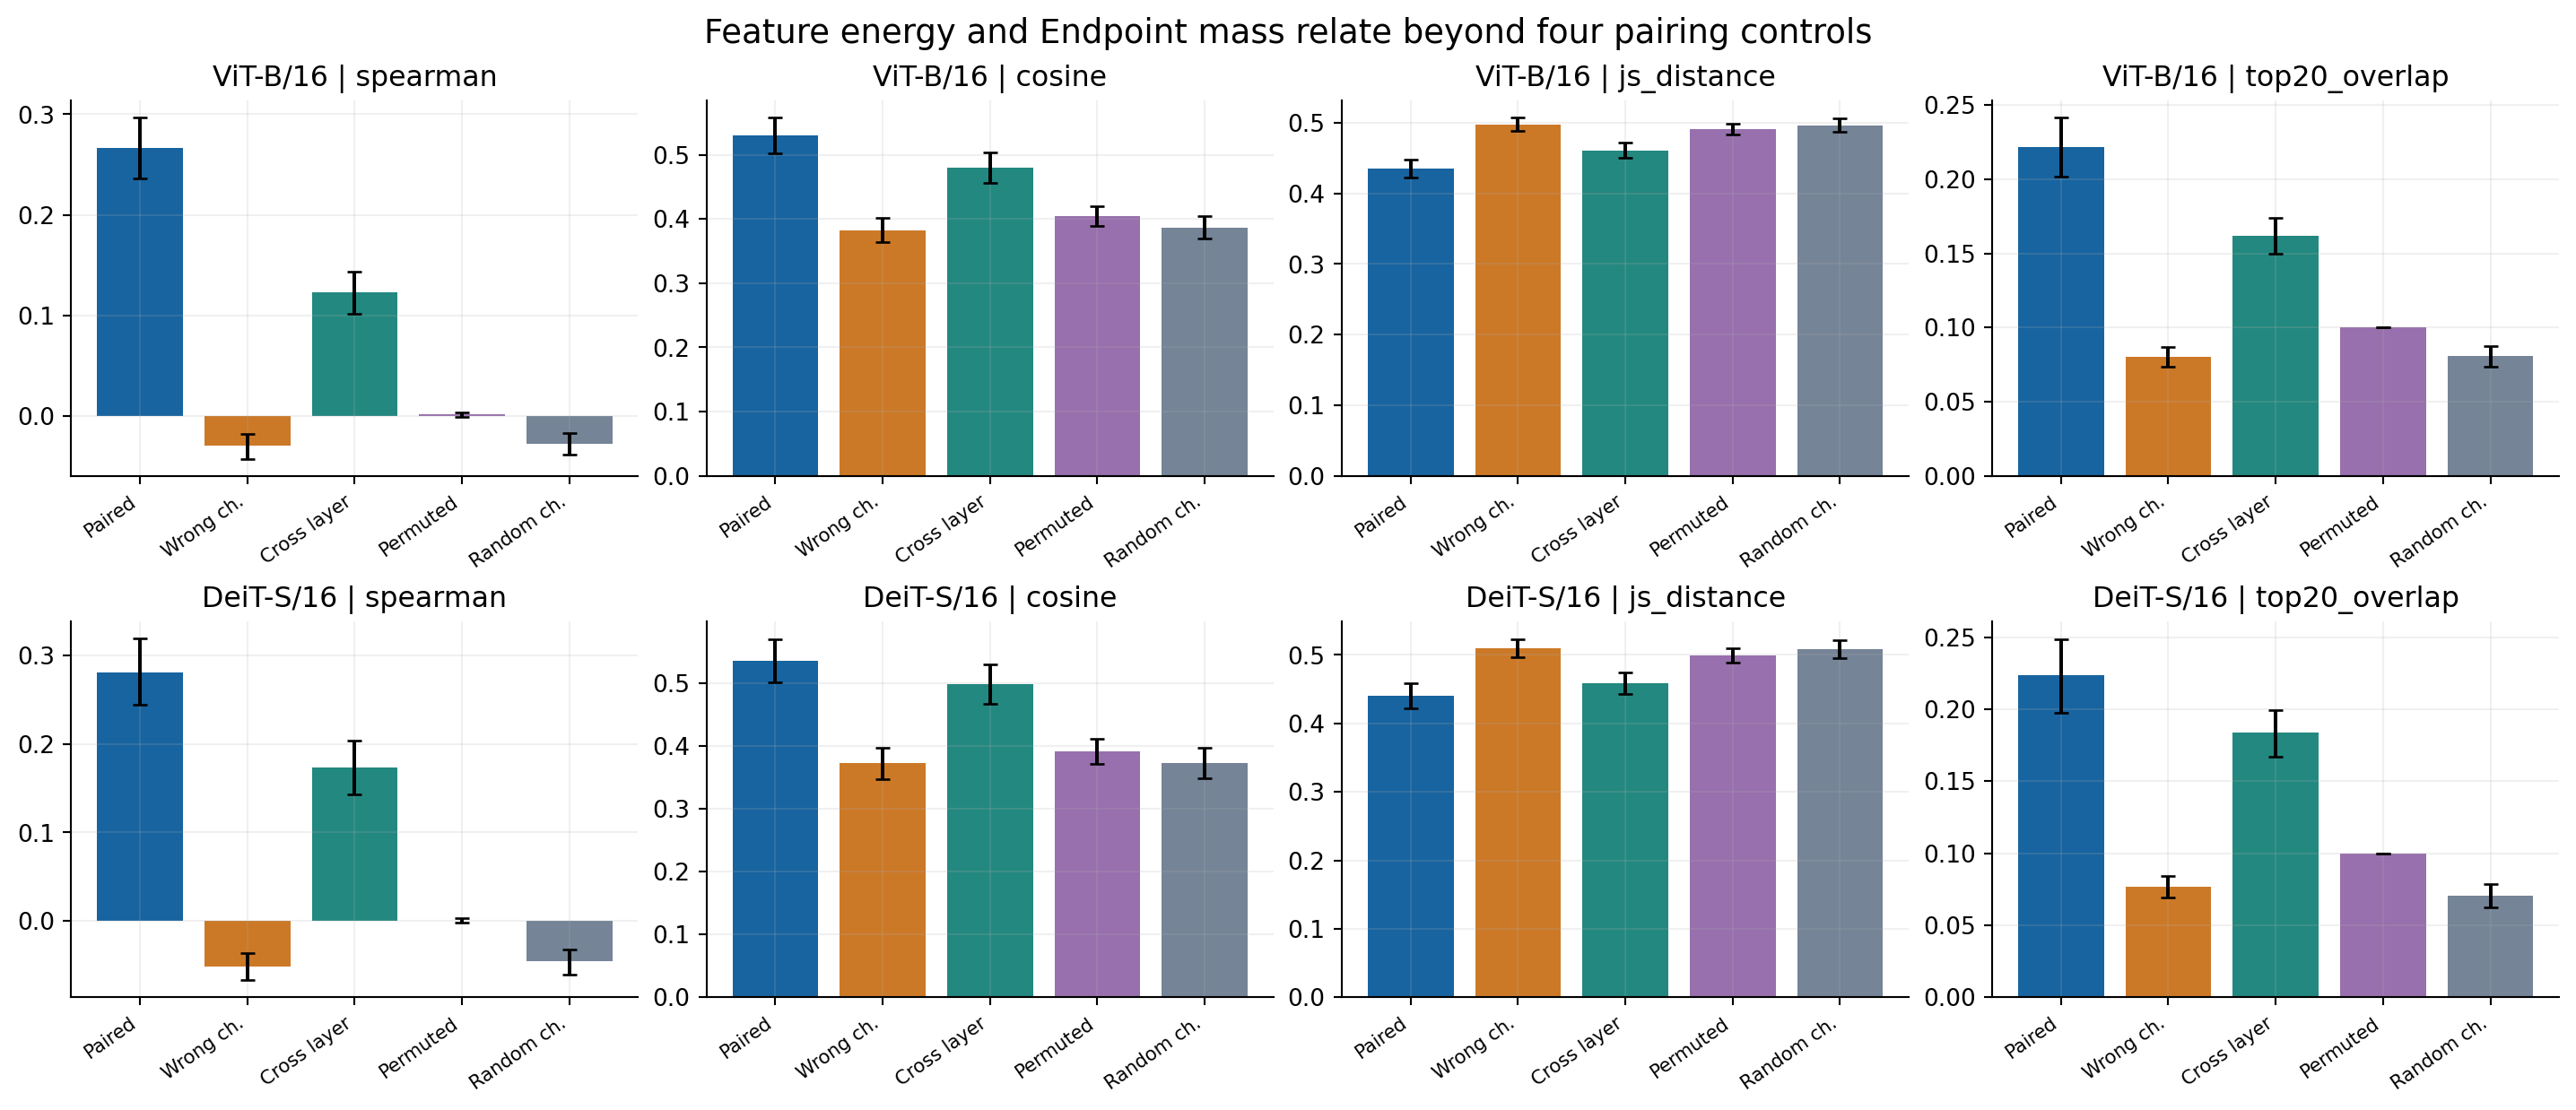
\includegraphics[keepaspectratio,alt={Supplement Figure 5}]{../evidence/supplement_v1/sup_05_feature_relation.png}}

{\def\LTcaptype{none} % do not increment counter
\begingroup\scriptsize
\setlength{\tabcolsep}{2pt}
\begin{longtable}[]{@{}
  >{\raggedright\arraybackslash}p{(\linewidth - 8\tabcolsep) * \real{0.2000}}
  >{\raggedright\arraybackslash}p{(\linewidth - 8\tabcolsep) * \real{0.2000}}
  >{\raggedright\arraybackslash}p{(\linewidth - 8\tabcolsep) * \real{0.2000}}
  >{\raggedright\arraybackslash}p{(\linewidth - 8\tabcolsep) * \real{0.2000}}
  >{\raggedright\arraybackslash}p{(\linewidth - 8\tabcolsep) * \real{0.2000}}@{}}
\toprule\noalign{}
\begin{minipage}[b]{\linewidth}\raggedright
Model
\end{minipage} & \begin{minipage}[b]{\linewidth}\raggedright
Pairing
\end{minipage} & \begin{minipage}[b]{\linewidth}\raggedright
Metric
\end{minipage} & \begin{minipage}[b]{\linewidth}\raggedright
Mean
\end{minipage} & \begin{minipage}[b]{\linewidth}\raggedright
95\% CI
\end{minipage} \\
\midrule\noalign{}
\endhead
\bottomrule\noalign{}
\endlastfoot
ViT-B/16 & paired & spearman & 0.2663 & {[}0.2366, 0.2973{]} \\
ViT-B/16 & wrong\_channel & spearman & -0.0298 & {[}-0.0426,
-0.0177{]} \\
ViT-B/16 & cross\_layer & spearman & 0.1232 & {[}0.1019, 0.1435{]} \\
ViT-B/16 & permuted & spearman & 0.0013 & {[}-0.0010, 0.0036{]} \\
ViT-B/16 & random\_channel & spearman & -0.0275 & {[}-0.0389,
-0.0175{]} \\
ViT-B/16 & paired & cosine & 0.5304 & {[}0.5029, 0.5575{]} \\
ViT-B/16 & wrong\_channel & cosine & 0.3826 & {[}0.3643, 0.4011{]} \\
ViT-B/16 & cross\_layer & cosine & 0.4802 & {[}0.4562, 0.5032{]} \\
ViT-B/16 & permuted & cosine & 0.4043 & {[}0.3888, 0.4198{]} \\
ViT-B/16 & random\_channel & cosine & 0.3868 & {[}0.3691, 0.4041{]} \\
ViT-B/16 & paired & js\_distance & 0.4351 & {[}0.4223, 0.4484{]} \\
ViT-B/16 & wrong\_channel & js\_distance & 0.4974 & {[}0.4884,
0.5070{]} \\
ViT-B/16 & cross\_layer & js\_distance & 0.4604 & {[}0.4498,
0.4716{]} \\
ViT-B/16 & permuted & js\_distance & 0.4909 & {[}0.4837, 0.4983{]} \\
ViT-B/16 & random\_channel & js\_distance & 0.4960 & {[}0.4869,
0.5059{]} \\
ViT-B/16 & paired & top20\_overlap & 0.2215 & {[}0.2016, 0.2414{]} \\
ViT-B/16 & wrong\_channel & top20\_overlap & 0.0805 & {[}0.0734,
0.0871{]} \\
ViT-B/16 & cross\_layer & top20\_overlap & 0.1621 & {[}0.1496,
0.1742{]} \\
ViT-B/16 & permuted & top20\_overlap & 0.1000 & {[}0.1000, 0.1000{]} \\
ViT-B/16 & random\_channel & top20\_overlap & 0.0809 & {[}0.0738,
0.0875{]} \\
DeiT-S/16 & paired & spearman & 0.2811 & {[}0.2442, 0.3191{]} \\
DeiT-S/16 & wrong\_channel & spearman & -0.0514 & {[}-0.0670,
-0.0361{]} \\
DeiT-S/16 & cross\_layer & spearman & 0.1735 & {[}0.1430, 0.2036{]} \\
DeiT-S/16 & permuted & spearman & 0.0003 & {[}-0.0021, 0.0029{]} \\
DeiT-S/16 & random\_channel & spearman & -0.0458 & {[}-0.0611,
-0.0318{]} \\
DeiT-S/16 & paired & cosine & 0.5359 & {[}0.5010, 0.5697{]} \\
DeiT-S/16 & wrong\_channel & cosine & 0.3723 & {[}0.3477, 0.3966{]} \\
DeiT-S/16 & cross\_layer & cosine & 0.4989 & {[}0.4673, 0.5300{]} \\
DeiT-S/16 & permuted & cosine & 0.3912 & {[}0.3718, 0.4111{]} \\
DeiT-S/16 & random\_channel & cosine & 0.3733 & {[}0.3490, 0.3974{]} \\
DeiT-S/16 & paired & js\_distance & 0.4406 & {[}0.4225, 0.4587{]} \\
DeiT-S/16 & wrong\_channel & js\_distance & 0.5094 & {[}0.4962,
0.5228{]} \\
DeiT-S/16 & cross\_layer & js\_distance & 0.4584 & {[}0.4429,
0.4740{]} \\
DeiT-S/16 & permuted & js\_distance & 0.4990 & {[}0.4886, 0.5098{]} \\
DeiT-S/16 & random\_channel & js\_distance & 0.5085 & {[}0.4958,
0.5218{]} \\
DeiT-S/16 & paired & top20\_overlap & 0.2234 & {[}0.1973, 0.2484{]} \\
DeiT-S/16 & wrong\_channel & top20\_overlap & 0.0770 & {[}0.0695,
0.0844{]} \\
DeiT-S/16 & cross\_layer & top20\_overlap & 0.1836 & {[}0.1668,
0.1992{]} \\
DeiT-S/16 & permuted & top20\_overlap & 0.1000 & {[}0.1000, 0.1000{]} \\
DeiT-S/16 & random\_channel & top20\_overlap & 0.0707 & {[}0.0625,
0.0785{]} \\
\end{longtable}
\endgroup
}

{\def\LTcaptype{none} % do not increment counter
\begingroup\scriptsize
\setlength{\tabcolsep}{2pt}
\begin{longtable}[]{@{}
  >{\raggedright\arraybackslash}p{(\linewidth - 8\tabcolsep) * \real{0.2000}}
  >{\raggedright\arraybackslash}p{(\linewidth - 8\tabcolsep) * \real{0.2000}}
  >{\raggedright\arraybackslash}p{(\linewidth - 8\tabcolsep) * \real{0.2000}}
  >{\raggedright\arraybackslash}p{(\linewidth - 8\tabcolsep) * \real{0.2000}}
  >{\raggedright\arraybackslash}p{(\linewidth - 8\tabcolsep) * \real{0.2000}}@{}}
\toprule\noalign{}
\begin{minipage}[b]{\linewidth}\raggedright
Model
\end{minipage} & \begin{minipage}[b]{\linewidth}\raggedright
Control
\end{minipage} & \begin{minipage}[b]{\linewidth}\raggedright
Metric
\end{minipage} & \begin{minipage}[b]{\linewidth}\raggedright
Paired similarity advantage
\end{minipage} & \begin{minipage}[b]{\linewidth}\raggedright
95\% CI
\end{minipage} \\
\midrule\noalign{}
\endhead
\bottomrule\noalign{}
\endlastfoot
ViT-B/16 & wrong\_channel & spearman & 0.2961 & {[}0.2763, 0.3165{]} \\
ViT-B/16 & cross\_layer & spearman & 0.1431 & {[}0.1292, 0.1579{]} \\
ViT-B/16 & permuted & spearman & 0.2649 & {[}0.2350, 0.2961{]} \\
ViT-B/16 & random\_channel & spearman & 0.2937 & {[}0.2709, 0.3183{]} \\
ViT-B/16 & wrong\_channel & cosine & 0.1478 & {[}0.1367, 0.1584{]} \\
ViT-B/16 & cross\_layer & cosine & 0.0502 & {[}0.0429, 0.0582{]} \\
ViT-B/16 & permuted & cosine & 0.1261 & {[}0.1126, 0.1391{]} \\
ViT-B/16 & random\_channel & cosine & 0.1436 & {[}0.1318, 0.1543{]} \\
ViT-B/16 & wrong\_channel & js\_distance & 0.0623 & {[}0.0579,
0.0666{]} \\
ViT-B/16 & cross\_layer & js\_distance & 0.0253 & {[}0.0220,
0.0286{]} \\
ViT-B/16 & permuted & js\_distance & 0.0558 & {[}0.0495, 0.0617{]} \\
ViT-B/16 & random\_channel & js\_distance & 0.0608 & {[}0.0562,
0.0654{]} \\
ViT-B/16 & wrong\_channel & top20\_overlap & 0.1410 & {[}0.1262,
0.1570{]} \\
ViT-B/16 & cross\_layer & top20\_overlap & 0.0594 & {[}0.0484,
0.0711{]} \\
ViT-B/16 & permuted & top20\_overlap & 0.1215 & {[}0.1016, 0.1414{]} \\
ViT-B/16 & random\_channel & top20\_overlap & 0.1406 & {[}0.1246,
0.1574{]} \\
DeiT-S/16 & wrong\_channel & spearman & 0.3325 & {[}0.3092, 0.3568{]} \\
DeiT-S/16 & cross\_layer & spearman & 0.1076 & {[}0.0975, 0.1181{]} \\
DeiT-S/16 & permuted & spearman & 0.2807 & {[}0.2430, 0.3192{]} \\
DeiT-S/16 & random\_channel & spearman & 0.3268 & {[}0.3009,
0.3532{]} \\
DeiT-S/16 & wrong\_channel & cosine & 0.1636 & {[}0.1527, 0.1741{]} \\
DeiT-S/16 & cross\_layer & cosine & 0.0370 & {[}0.0315, 0.0425{]} \\
DeiT-S/16 & permuted & cosine & 0.1447 & {[}0.1259, 0.1633{]} \\
DeiT-S/16 & random\_channel & cosine & 0.1626 & {[}0.1507, 0.1740{]} \\
DeiT-S/16 & wrong\_channel & js\_distance & 0.0687 & {[}0.0638,
0.0737{]} \\
DeiT-S/16 & cross\_layer & js\_distance & 0.0177 & {[}0.0146,
0.0207{]} \\
DeiT-S/16 & permuted & js\_distance & 0.0584 & {[}0.0501, 0.0663{]} \\
DeiT-S/16 & random\_channel & js\_distance & 0.0679 & {[}0.0628,
0.0730{]} \\
DeiT-S/16 & wrong\_channel & top20\_overlap & 0.1465 & {[}0.1262,
0.1660{]} \\
DeiT-S/16 & cross\_layer & top20\_overlap & 0.0398 & {[}0.0297,
0.0504{]} \\
DeiT-S/16 & permuted & top20\_overlap & 0.1234 & {[}0.0973, 0.1484{]} \\
DeiT-S/16 & random\_channel & top20\_overlap & 0.1527 & {[}0.1328,
0.1723{]} \\
\end{longtable}
\endgroup
}

\href{../evidence/supplement_v1/feature_unit_values.csv}{Unit metrics} ·
\href{../evidence/supplement_v1/feature_block_image_values.csv}{Image-block
values}

\section{S13. 抽样敏感性}\label{s13.-ux62bdux6837ux654fux611fux6027}

在相同 32 图上复用 M3 原 32 channels 和 15 patch strata。channel 与
token-stratum bootstrap 各 256 次，image bootstrap 2,000 次，并逐一移除
block 或空间
stratum。下表给出重采样分布和删除敏感性范围。前三个空间趋势方向在所有敏感性范围内保持一致。该分析没有生成独立
channel-seed 复现实验。CLS−patch 列为全层差值；其余为 late−early。

{\def\LTcaptype{none} % do not increment counter
\begingroup\scriptsize
\setlength{\tabcolsep}{2pt}
\begin{longtable}[]{@{}
  >{\raggedright\arraybackslash}p{(\linewidth - 14\tabcolsep) * \real{0.1250}}
  >{\raggedright\arraybackslash}p{(\linewidth - 14\tabcolsep) * \real{0.1250}}
  >{\raggedright\arraybackslash}p{(\linewidth - 14\tabcolsep) * \real{0.1250}}
  >{\raggedright\arraybackslash}p{(\linewidth - 14\tabcolsep) * \real{0.1250}}
  >{\raggedright\arraybackslash}p{(\linewidth - 14\tabcolsep) * \real{0.1250}}
  >{\raggedright\arraybackslash}p{(\linewidth - 14\tabcolsep) * \real{0.1250}}
  >{\raggedright\arraybackslash}p{(\linewidth - 14\tabcolsep) * \real{0.1250}}
  >{\raggedright\arraybackslash}p{(\linewidth - 14\tabcolsep) * \real{0.1250}}@{}}
\toprule\noalign{}
\begin{minipage}[b]{\linewidth}\raggedright
Model
\end{minipage} & \begin{minipage}[b]{\linewidth}\raggedright
Metric
\end{minipage} & \begin{minipage}[b]{\linewidth}\raggedright
Reference mean
\end{minipage} & \begin{minipage}[b]{\linewidth}\raggedright
Image CI
\end{minipage} & \begin{minipage}[b]{\linewidth}\raggedright
Channel bootstrap range
\end{minipage} & \begin{minipage}[b]{\linewidth}\raggedright
Token bootstrap range
\end{minipage} & \begin{minipage}[b]{\linewidth}\raggedright
Leave-one-block range
\end{minipage} & \begin{minipage}[b]{\linewidth}\raggedright
Leave-one-stratum range
\end{minipage} \\
\midrule\noalign{}
\endhead
\bottomrule\noalign{}
\endlastfoot
ViT-B/16 & entropy & 0.2392 & {[}0.2303, 0.2480{]} & {[}0.2307,
0.2472{]} & {[}0.2326, 0.2421{]} & {[}0.1847, 0.2937{]} & {[}0.2375,
0.2403{]} \\
ViT-B/16 & locality & -0.3607 & {[}-0.3683, -0.3526{]} & {[}-0.3678,
-0.3523{]} & {[}-0.3641, -0.3526{]} & {[}-0.4091, -0.3123{]} &
{[}-0.3617, -0.3596{]} \\
ViT-B/16 & distance & 0.1331 & {[}0.1274, 0.1389{]} & {[}0.1295,
0.1358{]} & {[}0.1168, 0.1478{]} & {[}0.1182, 0.1479{]} & {[}0.1296,
0.1366{]} \\
ViT-B/16 & cancellation & 0.0024 & {[}0.0021, 0.0028{]} & {[}0.0020,
0.0029{]} & {[}0.0022, 0.0027{]} & {[}0.0016, 0.0032{]} & {[}0.0024,
0.0025{]} \\
ViT-B/16 & cls\_minus\_patch\_entropy & 0.0564 & {[}0.0454, 0.0669{]} &
{[}0.0551, 0.0590{]} & {[}0.0527, 0.0636{]} & {[}0.0528, 0.0600{]} &
{[}0.0548, 0.0580{]} \\
DeiT-S/16 & entropy & 0.2236 & {[}0.2167, 0.2299{]} & {[}0.2190,
0.2279{]} & {[}0.2185, 0.2274{]} & {[}0.1800, 0.2673{]} & {[}0.2232,
0.2254{]} \\
DeiT-S/16 & locality & -0.3412 & {[}-0.3527, -0.3300{]} & {[}-0.3447,
-0.3376{]} & {[}-0.3494, -0.3315{]} & {[}-0.3797, -0.3026{]} &
{[}-0.3429, -0.3378{]} \\
DeiT-S/16 & distance & 0.1261 & {[}0.1191, 0.1338{]} & {[}0.1249,
0.1277{]} & {[}0.1138, 0.1381{]} & {[}0.1176, 0.1347{]} & {[}0.1239,
0.1304{]} \\
DeiT-S/16 & cancellation & 0.0020 & {[}0.0016, 0.0025{]} & {[}0.0018,
0.0022{]} & {[}0.0018, 0.0024{]} & {[}0.0014, 0.0025{]} & {[}0.0019,
0.0021{]} \\
DeiT-S/16 & cls\_minus\_patch\_entropy & 0.0829 & {[}0.0699, 0.0943{]} &
{[}0.0813, 0.0850{]} & {[}0.0741, 0.0931{]} & {[}0.0749, 0.0909{]} &
{[}0.0794, 0.0848{]} \\
\end{longtable}
\endgroup
}

\section{S14. 跨层全-head M2
与适用范围}\label{s14.-ux8de8ux5c42ux5168-head-m2-ux4e0eux9002ux7528ux8303ux56f4}

主文 block-5 三-head 实验对应原确认性协议。已封存 M2 覆盖 blocks
2/5/10、两模型、全部 heads、两种 references、每 family 400 图；原生
patch 几何下完整输入替换 11/12、单-head 隔离替换 12/12 显著偏向 regional
Taylor。下表使用原全部 672 个双向 AUC 检验的 Holm 校正，未重新定义检验
family。

{\def\LTcaptype{none} % do not increment counter
\begingroup\scriptsize
\setlength{\tabcolsep}{2pt}
\begin{longtable}[]{@{}
  >{\raggedright\arraybackslash}p{(\linewidth - 12\tabcolsep) * \real{0.1429}}
  >{\raggedright\arraybackslash}p{(\linewidth - 12\tabcolsep) * \real{0.1429}}
  >{\raggedright\arraybackslash}p{(\linewidth - 12\tabcolsep) * \real{0.1429}}
  >{\raggedright\arraybackslash}p{(\linewidth - 12\tabcolsep) * \real{0.1429}}
  >{\raggedright\arraybackslash}p{(\linewidth - 12\tabcolsep) * \real{0.1429}}
  >{\raggedright\arraybackslash}p{(\linewidth - 12\tabcolsep) * \real{0.1429}}
  >{\raggedright\arraybackslash}p{(\linewidth - 12\tabcolsep) * \real{0.1429}}@{}}
\toprule\noalign{}
\begin{minipage}[b]{\linewidth}\raggedright
Model
\end{minipage} & \begin{minipage}[b]{\linewidth}\raggedright
Reference
\end{minipage} & \begin{minipage}[b]{\linewidth}\raggedright
Block
\end{minipage} & \begin{minipage}[b]{\linewidth}\raggedright
Outcome
\end{minipage} & \begin{minipage}[b]{\linewidth}\raggedright
n images
\end{minipage} & \begin{minipage}[b]{\linewidth}\raggedright
Taylor \textgreater{} Endpoint Holm p
\end{minipage} & \begin{minipage}[b]{\linewidth}\raggedright
Supported
\end{minipage} \\
\midrule\noalign{}
\endhead
\bottomrule\noalign{}
\endlastfoot
DeiT-S/16 & blur & 10 & full & 400 & 5.841e-20 & True \\
DeiT-S/16 & blur & 10 & isolated & 400 & 2.355e-82 & True \\
DeiT-S/16 & normalized-zero & 10 & full & 400 & 0.0282 & True \\
DeiT-S/16 & normalized-zero & 10 & isolated & 400 & 4.045e-90 & True \\
DeiT-S/16 & blur & 2 & full & 400 & 1.103e-08 & True \\
DeiT-S/16 & blur & 2 & isolated & 400 & 6.597e-69 & True \\
DeiT-S/16 & normalized-zero & 2 & full & 400 & 0.04217 & True \\
DeiT-S/16 & normalized-zero & 2 & isolated & 400 & 2.276e-58 & True \\
DeiT-S/16 & blur & 5 & full & 400 & 6.793e-15 & True \\
DeiT-S/16 & blur & 5 & isolated & 400 & 7.52e-85 & True \\
DeiT-S/16 & normalized-zero & 5 & full & 400 & 0.5283 & False \\
DeiT-S/16 & normalized-zero & 5 & isolated & 400 & 2.355e-82 & True \\
ViT-B/16 & blur & 10 & full & 400 & 5.562e-28 & True \\
ViT-B/16 & blur & 10 & isolated & 400 & 2.351e-94 & True \\
ViT-B/16 & normalized-zero & 10 & full & 400 & 2.309e-26 & True \\
ViT-B/16 & normalized-zero & 10 & isolated & 400 & 2.424e-97 & True \\
ViT-B/16 & blur & 2 & full & 400 & 4.341e-16 & True \\
ViT-B/16 & blur & 2 & isolated & 400 & 6.185e-64 & True \\
ViT-B/16 & normalized-zero & 2 & full & 400 & 2.49e-17 & True \\
ViT-B/16 & normalized-zero & 2 & isolated & 400 & 7.981e-47 & True \\
ViT-B/16 & blur & 5 & full & 400 & 2.591e-25 & True \\
ViT-B/16 & blur & 5 & isolated & 400 & 1.679e-91 & True \\
ViT-B/16 & normalized-zero & 5 & full & 400 & 9.405e-18 & True \\
ViT-B/16 & normalized-zero & 5 & isolated & 400 & 1.042e-115 & True \\
\end{longtable}
\endgroup
}

本轮未执行可选 cascading randomization、P2 同目标 M3--M4 桥接、独立
channel seeds、替代 checkpoint，或 P3 输入变换与 CNN
展示。本文不把训练对照解释为有限因果机制，也不把不同标量目标之间的总体关联解释为逐单元桥接。Path
IG 的原冻结校准失败及原确认性结论保持不变。

\href{../evidence/supplement_v1/protocol.md}{Frozen protocol} ·
\href{../evidence/supplement_v1/source_bindings.json}{Source bindings} ·
\href{../evidence/supplement_v1/acquisition_receipt.json}{Task
acquisition} ·
\href{../evidence/supplement_v1/validation_report.json}{Numerical
validation}

\# S15. 数据、模型、总体与分析身份

ImageNet 来源为 ILSVRC2012 官方验证集。模型由 timm 0.9.16 标准
Block/Attention 实例化并严格加载权重，所有权重文件已重新核验大小和
SHA-256。AugReg 名称标明 IN21K 预训练后 IN1K 微调或 IN1K 训练；DeiT-S
使用公开 Facebook IN1K 参数。所有结果条件于这些参数状态。

{\def\LTcaptype{none} % do not increment counter
\begingroup\scriptsize
\setlength{\tabcolsep}{2pt}
\begin{longtable}[]{@{}
  >{\raggedright\arraybackslash}p{(\linewidth - 6\tabcolsep) * \real{0.2500}}
  >{\raggedright\arraybackslash}p{(\linewidth - 6\tabcolsep) * \real{0.2500}}
  >{\raggedright\arraybackslash}p{(\linewidth - 6\tabcolsep) * \real{0.2500}}
  >{\raggedright\arraybackslash}p{(\linewidth - 6\tabcolsep) * \real{0.2500}}@{}}
\toprule\noalign{}
\begin{minipage}[b]{\linewidth}\raggedright
Model ID
\end{minipage} & \begin{minipage}[b]{\linewidth}\raggedright
Exact timm name / training
\end{minipage} & \begin{minipage}[b]{\linewidth}\raggedright
Bytes
\end{minipage} & \begin{minipage}[b]{\linewidth}\raggedright
SHA-256
\end{minipage} \\
\midrule\noalign{}
\endhead
\bottomrule\noalign{}
\endlastfoot
vit\_b16 & vit\_base\_patch16\_224.augreg2\_in21k\_ft\_in1k & 346329934
& 489bfa2f1aa3b6781e268a87eb629816b89eebba439420978a794b8e8151565d \\
deit\_s16 & deit\_small\_patch16\_224.fb\_in1k & 88251143 &
cd65a15597004d0ce19d7a9daef969903972db5b398e3a5febcd3c4df1d8f59f \\
vit\_b16\_in1k & vit\_base\_patch16\_224.augreg\_in1k & 346335542 &
69c9a2822a47838f57e522350b10ccc0d89d67fdcee07603e4ae3259b3350336 \\
vit\_s16\_augreg & vit\_small\_patch16\_224.augreg\_in21k\_ft\_in1k &
88267574 &
545815b4e770d2fa6ca4b3ccba7c16b035e474354e52d17ca197ea4efecbf4d3 \\
\end{longtable}
\endgroup
}

原 discovery、calibration、evaluation 分别 64、64、400
类，每类一图。Unit-study 的 100 类各一图是 evaluation 子集。E1 为 100
类各五图，E5 为 400 类各一图。E5 从排除历史曝光和 E1 的候选集中按
class\_e5/image\_e5
哈希排序选择。以下矩阵报告图像身份重叠；同类别可以跨后续队列出现，图像独立不等于类别独立。E5
的 train/validation/test 标签用于另一个预测分析，不改变此处全部 400 图
H1--H4 检查。

{\def\LTcaptype{none} % do not increment counter
\begingroup\scriptsize
\setlength{\tabcolsep}{2pt}
\begin{longtable}[]{@{}lllllll@{}}
\toprule\noalign{}
Cohort & discovery & calibration & evaluation & unit\_study & e1 & e5 \\
\midrule\noalign{}
\endhead
\bottomrule\noalign{}
\endlastfoot
discovery & 64 & 0 & 0 & 0 & 0 & 0 \\
calibration & 0 & 64 & 0 & 0 & 0 & 0 \\
evaluation & 0 & 0 & 400 & 100 & 0 & 0 \\
unit\_study & 0 & 0 & 100 & 100 & 0 & 0 \\
e1 & 0 & 0 & 0 & 0 & 500 & 0 \\
e5 & 0 & 0 & 0 & 0 & 0 & 400 \\
\end{longtable}
\endgroup
}

预处理使用 Pillow 10.2.0 RGB，不应用 EXIF transpose。Torchvision 0.17.2
先对 PIL 图像以 bicubic 将短边 resize 到 248，antialias=True，再中心
crop 224，转 float32 并除 255。每模型 normalization 使用 Table 2
参数。Blur 在 crop 后 RGB 上使用 31×31 Gaussian
kernel、sigma=10、reflect padding=15，再 normalization。Evaluation mode
关闭 dropout 和 drop path。CLS、位置编码与 bias 固定。原 logit
目标为官方 ground-truth，clean-top1 为另一个预先固定读出；它们不参与
cohort 选择。原 registry 每层四 tokens/四 channels
的规则和实际列表由封存 registry 给出。M3 固定 CLS 加 15 个 3×5 分层
tokens，每层 32
channels；跨模型同序号不代表同一语义神经元。结构研究扫描全部 heads 和 12
blocks，区域主任务为 block 5，ViT-B heads 0/6/11、DeiT-S heads 0/3/5。

所有抽样是确定性规则或公开种子。实际 selected IDs 与 targets 由
\href{../evidence/revision_v6/cohort_bindings.json}{cohort bindings}
提供。随机控制的具体派生键与调用顺序保留于原协议，不能把不同分析的种子混用。

{\def\LTcaptype{none} % do not increment counter
\begingroup\scriptsize
\setlength{\tabcolsep}{2pt}
\begin{longtable}[]{@{}
  >{\raggedright\arraybackslash}p{(\linewidth - 2\tabcolsep) * \real{0.5000}}
  >{\raggedright\arraybackslash}p{(\linewidth - 2\tabcolsep) * \real{0.5000}}@{}}
\toprule\noalign{}
\begin{minipage}[b]{\linewidth}\raggedright
Purpose
\end{minipage} & \begin{minipage}[b]{\linewidth}\raggedright
Frozen seed / deterministic rule
\end{minipage} \\
\midrule\noalign{}
\endhead
\bottomrule\noalign{}
\endlastfoot
Original image selection & SHA256(NNS\_VIT\_ENDPOINT\_EP0\_R1\_20260918
\textbar{} class \textbar{} WNID), then namespace \textbar{} image
\textbar{} filename \\
Unit cohort & SHA256(ENDPOINT\_M3\_COHORT\_20260919 \textbar{}
sample\_id \textbar{} image\_sha256), lowest 100 \\
Unit channels & SHA256(ENDPOINT\_M3\_CHANNEL\_20260919 \textbar{} model
\textbar{} block \textbar{} channel), lowest 32 \\
Unit tokens & CLS + nearest patch to each of 3×5 strata centers;
row-major ties \\
Original bootstrap & SHA256(namespace \textbar{} bootstrap \textbar{}
family\_id), first 8 bytes big-endian; PCG64 \\
Unit bootstrap & SHA256(ENDPOINT\_M3\_BOOTSTRAP\_20260919 \textbar{} M3
\textbar{} model \textbar{} metric), first 8 bytes \\
Structural bootstrap & SHA256(M4 \textbar{} test \textbar{} model
\textbar{} test\_id), with residual type inserted where applicable \\
Random initialization & 202609201, 202609202, 202609203 \\
Independent cohort / target selection &
NNS\_VIT\_REVISION\_V5\_20260921\_R1 namespace; class\_e5, image\_e5 and
post/block/channel/token keys \\
Independent-cohort bootstrap & ENDPOINT\_M1\_20260918\_V1 \textbar{}
20260918 \textbar{} bootstrap \textbar{} V5 \textbar{}
(model,hypothesis) \\
Coordinate/threshold bootstrap & SHA256(2026092302 \textbar{} analysis
key), first 8 bytes; 10,000 PCG64 replicates \\
Analytic directions & NumPy default\_rng(2026092301), three normalized
Gaussian directions \\
Regional random orders & Frozen
namespace/model/image/reference/head/repeat keys in original
intervention registry; 20 repeats \\
\end{longtable}
\endgroup
}

确认性身份相对于各自分析前的本地冻结计划。外部公开注册未提供。下表保留各
family 的原成员与用途；后续检查不与原 28 项追溯合并。完整 28 个 test IDs
与所有 SHA-256 位于
\href{../evidence/revision_v6/analysis_identity.json}{analysis
identity}。0.10/0.05
没有外部效用校准来源，属于研究者操作阈值。原判断要求有效性、完整覆盖、n
和区间精度门，以及点估计和 Holm 检验共同通过；不要求 CI lower
\textgreater{} 0.10。阈值敏感性见
\href{../evidence/revision_v6/threshold_sensitivity.csv}{68
行完整结果}。

{\def\LTcaptype{none} % do not increment counter
\begingroup\scriptsize
\setlength{\tabcolsep}{2pt}
\begin{longtable}[]{@{}
  >{\raggedright\arraybackslash}p{(\linewidth - 6\tabcolsep) * \real{0.2500}}
  >{\raggedright\arraybackslash}p{(\linewidth - 6\tabcolsep) * \real{0.2500}}
  >{\raggedright\arraybackslash}p{(\linewidth - 6\tabcolsep) * \real{0.2500}}
  >{\raggedright\arraybackslash}p{(\linewidth - 6\tabcolsep) * \real{0.2500}}@{}}
\toprule\noalign{}
\begin{minipage}[b]{\linewidth}\raggedright
Analysis
\end{minipage} & \begin{minipage}[b]{\linewidth}\raggedright
Identity
\end{minipage} & \begin{minipage}[b]{\linewidth}\raggedright
Multiplicity family
\end{minipage} & \begin{minipage}[b]{\linewidth}\raggedright
Local freeze evidence
\end{minipage} \\
\midrule\noalign{}
\endhead
\bottomrule\noalign{}
\endlastfoot
original\_component\_and\_region & confirmatory & 28 tests jointly Holm;
12 component correlations + 16 regional baseline contrasts & local
pre-outcome plan; first committed occurrence below;
6237ef87a1af0205973b76bee172defe33a0a6da 2026-09-18T09:26:20+08:00 \\
unit\_depth & confirmatory & five per model: entropy, locality,
distance, cancellation, CLS-patch entropy & local pre-outcome plan;
first committed occurrence below;
f2eba3f60d765e6a9729d9ff12a57bd01f93f952 2026-09-19T13:53:48+08:00 \\
attention\_residual\_depth & confirmatory & four attention tests/model;
two residual tests/model/type & local pre-outcome plan; first committed
occurrence below; 1a1000bcdd15d8b0e76406f4376a82d60ec79b86
2026-09-19T17:25:17+08:00 \\
head\_baselines & exploratory & separate paired and absolute Spearman
families; other metrics descriptive & local pre-outcome plan; first
committed occurrence below; 33c8c320446a631b2e451016b3268eefdd9c926b
2026-09-19T04:20:36+08:00 \\
residual\_spatial\_tv & post-hoc & four Holm contrasts across model and
residual type & 2026-09-19T10:59:17.569991+00:00; protocol timestamp and
hashes \\
QKV\_spatial & prospective robustness & 30 descriptive contrasts; no
confirmatory family combined with prior tests &
2026-09-20T17:14:57.250515+00:00; protocol timestamp and hashes \\
independent\_cohort\_checkpoints & prospective robustness & H1-H4 Holm
separately within each checkpoint & local pre-outcome plan; first
committed occurrence below; 944f54c99c8d83803d461224565b93a779e75915
2026-09-21T11:31:10+08:00 \\
training\_target\_sampling\_controls & exploratory & descriptive 2000
bootstrap; training control resamples image and initialization seed;
sampling control resamples target strata and images &
2026-09-20T00:22:59.620440+00:00;
395d30b3804983d0e51e99a28d0c3c900aca8fda 2026-09-20T22:41:48+08:00 \\
coordinate\_sensitivity\_v6 & prospective robustness & no
significance-based success criterion; report all directions and
intervals & 2026-09-22T16:43:58.690139+00:00; protocol timestamp and
hashes \\
threshold\_sensitivity\_v6 & post-hoc & descriptive thresholds only;
original tests and decisions immutable &
2026-09-22T16:43:58.690139+00:00; protocol timestamp and hashes \\
\end{longtable}
\endgroup
}

\# S16. 有限替换变量与可执行伪代码

A 和 V 是前向变量，routing-induced/value-induced 是微分分组。Table 6 的
A/V family 每个 block 各一个全-head A 替换和 V 替换，共 24 成分；head
family 为所有 block/head，residual family 每 block attention 与 MLP
branch 各一项。Reference activation 来自完整 reference forward。下面的
consumer slot 是替换身份的一部分。

{\def\LTcaptype{none} % do not increment counter
\begingroup\scriptsize
\setlength{\tabcolsep}{2pt}
\begin{longtable}[]{@{}
  >{\raggedright\arraybackslash}p{(\linewidth - 6\tabcolsep) * \real{0.2500}}
  >{\raggedright\arraybackslash}p{(\linewidth - 6\tabcolsep) * \real{0.2500}}
  >{\raggedright\arraybackslash}p{(\linewidth - 6\tabcolsep) * \real{0.2500}}
  >{\raggedright\arraybackslash}p{(\linewidth - 6\tabcolsep) * \real{0.2500}}@{}}
\toprule\noalign{}
\begin{minipage}[b]{\linewidth}\raggedright
Replacement
\end{minipage} & \begin{minipage}[b]{\linewidth}\raggedright
Forward tensor / shape (batch=1)
\end{minipage} & \begin{minipage}[b]{\linewidth}\raggedright
Consumer input slot
\end{minipage} & \begin{minipage}[b]{\linewidth}\raggedright
Clean state and recomputation
\end{minipage} \\
\midrule\noalign{}
\endhead
\bottomrule\noalign{}
\endlastfoot
Attention probability & A {[}1,H,197,197{]}, after softmax/dropout &
left input of A @ V & V, other branches and residual identity clean;
recompute AV, concat, output projection, residual suffix \\
V projection & V {[}1,H,197,64{]}, qkv projection slice & right input of
A @ V & Q/K/A and identity clean; recompute AV and entire suffix \\
Head output & slice of projection\_input {[}1,197,H×64{]}, head h
channels h×64:(h+1)×64 & attn.proj input channels & all other head
slices and residual identity clean; recompute projection and suffix \\
Attention branch & drop\_path1 output {[}1,197,D{]} & residual1 add
branch input & identity u clean; recompute residual sum, MLP and
remaining blocks \\
MLP branch & drop\_path2 output {[}1,197,D{]} & residual2 add branch
input & carry r1 clean; recompute residual sum and remaining blocks \\
\end{longtable}
\endgroup
}

\begin{verbatim}
clean_rgb = RGB(image) / 255
clean_rgb = center_crop(resize_shorter_side(clean_rgb, 248, bicubic, antialias=True), 224)
x = (clean_rgb - mu) / sigma
reference_zero = zeros_like(x)             # raw RGB equals mu
reference_blur = (GaussianBlur(clean_rgb, kernel=31, sigma=10, reflect_padding=15) - mu) / sigma
clean = forward_and_capture(x)
reference = forward_and_capture(reference_input)
for fixed block, component, consumer slot:
    replacement = reference.tensor_at(component, slot)
    patched = forward(x, replace_only_this_use=replacement)
    effect = clean.GT_logit - patched.GT_logit
    # All sibling heads and bypass inputs remain clean before the replacement.
    # Every node downstream of the replaced use is recomputed normally.

for singleton region P in the fixed 4x4 grid of 56x56 pixels:
    x_P = x.copy(); x_P[P] = reference_input[P]
    mixed[P] = forward_and_capture(x_P)
    regional_Taylor[P] = abs(dot(clean_head_cotangent, clean_head - mixed[P].head))
rank_regions(score, ties=ascending_region_id)
for budget in [1, 2, 4]:
    selected = top_regions(budget)
    x_selected = x with selected pixels from reference_input
    mixed = forward_and_capture(x_selected)
    full_input_effect = clean.GT_logit - mixed.GT_logit
    isolated = forward(x, target_head_slice=mixed.head_slice)
    isolated_effect = clean.GT_logit - isolated.GT_logit
AUC = trapezoid(abs(isolated_effect), areas=[0,1/16,2/16,4/16]) / 0.25
image_AUC = mean(AUC across the three fixed heads)
random_AUC = mean(AUC per random repeat, then heads) # abs before averaging repeats
\end{verbatim}

Full-input effect 改变整条前向计算；isolated-component effect 只将 mixed
forward 的目标张量放入 clean forward，其他 head 与 bypass 保持
clean。区域分数的候选集合相同，但 Taylor 需额外 singleton mixed
forwards，因此信息预算不同。区域 ties 用编号升序，head ties 用 component
ID 升序，Spearman 用平均秩。所谓 candidate-envelope AUC
是在每个面积点从已评价候选中取最大 absolute effect，再积分、平均
heads，可能拼接不同排序的点，因此不是一条可执行的全局最优区域策略。它只用作已评价集合的上界和
regret 分母。

\# S17. 坐标敏感性与独立解析检查

三种表示均在同一当前输入点、同一固定目标与 checkpoint 上计算。Raw
gradient 除去模型 sigma；common-origin weighted gradient 使用原始 RGB
零点，不随模型 mean 改变。以下每格为图像级中位差和 95\% bootstrap
CI。Unit 每模型 n=100，结构项 n=400；缺失图像为零。每个 coordinate
在图内配对，不作为额外样本。

\begin{equation}\label{eq:zh-supplement-003}
E_i^{(x)}=x_i\frac{\partial s}{\partial x_i},\qquad
G_i^{(r)}=\frac1{\sigma_i}\frac{\partial s}{\partial x_i},\qquad
E_i^{(0)}=r_i\frac{\partial s}{\partial r_i}
=\left(x_i+\frac{\mu_i}{\sigma_i}\right)\frac{\partial s}{\partial x_i}.
\end{equation}

{\def\LTcaptype{none} % do not increment counter
\begingroup\scriptsize
\setlength{\tabcolsep}{2pt}
\begin{longtable}[]{@{}
  >{\raggedright\arraybackslash}p{(\linewidth - 12\tabcolsep) * \real{0.1429}}
  >{\raggedright\arraybackslash}p{(\linewidth - 12\tabcolsep) * \real{0.1429}}
  >{\raggedright\arraybackslash}p{(\linewidth - 12\tabcolsep) * \real{0.1429}}
  >{\raggedright\arraybackslash}p{(\linewidth - 12\tabcolsep) * \real{0.1429}}
  >{\raggedright\arraybackslash}p{(\linewidth - 12\tabcolsep) * \real{0.1429}}
  >{\raggedright\arraybackslash}p{(\linewidth - 12\tabcolsep) * \real{0.1429}}
  >{\raggedright\arraybackslash}p{(\linewidth - 12\tabcolsep) * \real{0.1429}}@{}}
\toprule\noalign{}
\begin{minipage}[b]{\linewidth}\raggedright
Model
\end{minipage} & \begin{minipage}[b]{\linewidth}\raggedright
Object / metric
\end{minipage} & \begin{minipage}[b]{\linewidth}\raggedright
Contrast
\end{minipage} & \begin{minipage}[b]{\linewidth}\raggedright
Normalized Endpoint
\end{minipage} & \begin{minipage}[b]{\linewidth}\raggedright
Raw-pixel gradient
\end{minipage} & \begin{minipage}[b]{\linewidth}\raggedright
Common-origin gradient
\end{minipage} & \begin{minipage}[b]{\linewidth}\raggedright
n / NA
\end{minipage} \\
\midrule\noalign{}
\endhead
\bottomrule\noalign{}
\endlastfoot
deit\_s16 & K / entropy & block11\_minus\_block0 & -0.067 {[}-0.074,
-0.059{]} & -0.066 {[}-0.073, -0.060{]} & -0.061 {[}-0.069, -0.053{]} &
400 / 0 \\
deit\_s16 & K / entropy & late\_minus\_early & -0.028 {[}-0.031,
-0.024{]} & -0.029 {[}-0.032, -0.026{]} & -0.027 {[}-0.031, -0.024{]} &
400 / 0 \\
deit\_s16 & Q / entropy & block11\_minus\_block0 & -0.004 {[}-0.008,
0.0005{]} & 0.003 {[}-0.001, 0.006{]} & 0.002 {[}-0.003, 0.006{]} & 400
/ 0 \\
deit\_s16 & Q / entropy & late\_minus\_early & 0.018 {[}0.013, 0.022{]}
& 0.018 {[}0.015, 0.022{]} & 0.015 {[}0.012, 0.018{]} & 400 / 0 \\
deit\_s16 & V / entropy & block11\_minus\_block0 & -0.067 {[}-0.075,
-0.061{]} & -0.076 {[}-0.081, -0.068{]} & -0.070 {[}-0.077, -0.062{]} &
400 / 0 \\
deit\_s16 & V / entropy & late\_minus\_early & -0.013 {[}-0.016,
-0.011{]} & -0.016 {[}-0.017, -0.013{]} & -0.015 {[}-0.017, -0.013{]} &
400 / 0 \\
deit\_s16 & attention / output\_identity\_tv & block11\_minus\_block0 &
0.078 {[}0.072, 0.085{]} & 0.079 {[}0.070, 0.085{]} & 0.074 {[}0.067,
0.081{]} & 400 / 0 \\
deit\_s16 & attention / output\_identity\_tv & late\_minus\_early &
0.028 {[}0.026, 0.030{]} & 0.028 {[}0.026, 0.030{]} & 0.027 {[}0.026,
0.029{]} & 400 / 0 \\
deit\_s16 & mlp / output\_identity\_tv & block11\_minus\_block0 & -0.050
{[}-0.059, -0.040{]} & -0.044 {[}-0.057, -0.037{]} & -0.037 {[}-0.043,
-0.029{]} & 400 / 0 \\
deit\_s16 & mlp / output\_identity\_tv & late\_minus\_early & -0.046
{[}-0.052, -0.041{]} & -0.044 {[}-0.051, -0.039{]} & -0.039 {[}-0.044,
-0.034{]} & 400 / 0 \\
deit\_s16 & unit / distance & block11\_minus\_block0 & 0.163 {[}0.159,
0.169{]} & 0.169 {[}0.164, 0.175{]} & 0.171 {[}0.167, 0.178{]} & 100 /
0 \\
deit\_s16 & unit / distance & late\_minus\_early & 0.122 {[}0.120,
0.128{]} & 0.129 {[}0.126, 0.132{]} & 0.127 {[}0.122, 0.131{]} & 100 /
0 \\
deit\_s16 & unit / entropy & block11\_minus\_block0 & 0.397 {[}0.387,
0.404{]} & 0.426 {[}0.412, 0.438{]} & 0.418 {[}0.400, 0.427{]} & 100 /
0 \\
deit\_s16 & unit / entropy & late\_minus\_early & 0.225 {[}0.212,
0.228{]} & 0.245 {[}0.241, 0.249{]} & 0.221 {[}0.217, 0.229{]} & 100 /
0 \\
deit\_s16 & unit / locality & block11\_minus\_block0 & -0.455 {[}-0.467,
-0.432{]} & -0.453 {[}-0.469, -0.441{]} & -0.477 {[}-0.493, -0.455{]} &
100 / 0 \\
deit\_s16 & unit / locality & late\_minus\_early & -0.342 {[}-0.353,
-0.333{]} & -0.359 {[}-0.366, -0.352{]} & -0.356 {[}-0.361, -0.344{]} &
100 / 0 \\
vit\_b16 & K / entropy & block11\_minus\_block0 & -0.059 {[}-0.064,
-0.053{]} & -0.052 {[}-0.058, -0.048{]} & -0.046 {[}-0.054, -0.041{]} &
400 / 0 \\
vit\_b16 & K / entropy & late\_minus\_early & -0.021 {[}-0.024,
-0.019{]} & -0.019 {[}-0.023, -0.016{]} & -0.019 {[}-0.022, -0.016{]} &
400 / 0 \\
vit\_b16 & Q / entropy & block11\_minus\_block0 & 0.027 {[}0.022,
0.031{]} & 0.026 {[}0.018, 0.031{]} & 0.014 {[}0.009, 0.018{]} & 400 /
0 \\
vit\_b16 & Q / entropy & late\_minus\_early & 0.037 {[}0.033, 0.043{]} &
0.039 {[}0.033, 0.044{]} & 0.034 {[}0.030, 0.037{]} & 400 / 0 \\
vit\_b16 & V / entropy & block11\_minus\_block0 & -0.053 {[}-0.059,
-0.047{]} & -0.057 {[}-0.061, -0.049{]} & -0.055 {[}-0.060, -0.050{]} &
400 / 0 \\
vit\_b16 & V / entropy & late\_minus\_early & -0.010 {[}-0.012,
-0.008{]} & -0.009 {[}-0.011, -0.007{]} & -0.010 {[}-0.012, -0.007{]} &
400 / 0 \\
vit\_b16 & attention / output\_identity\_tv & block11\_minus\_block0 &
0.166 {[}0.159, 0.172{]} & 0.167 {[}0.159, 0.174{]} & 0.167 {[}0.160,
0.175{]} & 400 / 0 \\
vit\_b16 & attention / output\_identity\_tv & late\_minus\_early & 0.052
{[}0.049, 0.055{]} & 0.054 {[}0.051, 0.056{]} & 0.053 {[}0.050, 0.055{]}
& 400 / 0 \\
vit\_b16 & mlp / output\_identity\_tv & block11\_minus\_block0 & -0.037
{[}-0.043, -0.031{]} & -0.034 {[}-0.038, -0.029{]} & -0.032 {[}-0.039,
-0.025{]} & 400 / 0 \\
vit\_b16 & mlp / output\_identity\_tv & late\_minus\_early & -0.019
{[}-0.022, -0.015{]} & -0.017 {[}-0.020, -0.013{]} & -0.018 {[}-0.021,
-0.014{]} & 400 / 0 \\
vit\_b16 & unit / distance & block11\_minus\_block0 & 0.197 {[}0.190,
0.204{]} & 0.205 {[}0.200, 0.211{]} & 0.209 {[}0.203, 0.214{]} & 100 /
0 \\
vit\_b16 & unit / distance & late\_minus\_early & 0.131 {[}0.129,
0.136{]} & 0.138 {[}0.134, 0.141{]} & 0.134 {[}0.129, 0.138{]} & 100 /
0 \\
vit\_b16 & unit / entropy & block11\_minus\_block0 & 0.398 {[}0.392,
0.409{]} & 0.440 {[}0.426, 0.447{]} & 0.412 {[}0.402, 0.426{]} & 100 /
0 \\
vit\_b16 & unit / entropy & late\_minus\_early & 0.220 {[}0.211,
0.227{]} & 0.240 {[}0.235, 0.246{]} & 0.217 {[}0.209, 0.223{]} & 100 /
0 \\
vit\_b16 & unit / locality & block11\_minus\_block0 & -0.526 {[}-0.534,
-0.516{]} & -0.543 {[}-0.554, -0.532{]} & -0.545 {[}-0.552, -0.538{]} &
100 / 0 \\
vit\_b16 & unit / locality & late\_minus\_early & -0.356 {[}-0.363,
-0.350{]} & -0.367 {[}-0.373, -0.361{]} & -0.356 {[}-0.364, -0.347{]} &
100 / 0 \\
\end{longtable}
\endgroup
}

DeiT-S Q 的 B11−B0 在三坐标下的点估计符号不同且三个区间跨零。Phase
contrast 与 B11−B0 的差异还说明，终点比较不能替代整个轨迹。主文始终限定
normalized-input
Endpoint。其他对象只作这三表示下的方向保持判断，不推出一般参数化不变性。

独立参考以 NumPy float64 显式构造 affine、LayerNorm、softmax
\(\operatorname{diag}(a)-aa^{\mathsf T}\)、Q/K/V、head concat/output
projection、GELU/MLP 和 residual identity Jacobian。参考模块不导入
scanner、hook 或
autograd。独立驱动将其结果与实际主扫描器在单头、双头、pre-LN residual
attention/MLP tiny 模型上逐项比较。32 个分量比较和 9
个冻结方向有限差分通过，最大分量绝对误差 \(1.11\times10^{-16}\)；每项
relative L2 和容差见
\href{../evidence/revision_v6/analytic_reference_results.json}{analytic
results}。共享 producer 双 slot toy、Q/K slot 交换、提前合并 fan-out
和重复合并项均被拒绝，正确实现先通过。此能力限于这些数值图和故障类型，不等于排除全部
scanner 实现错误。

原区域数组键 raw\_gradient 记录 \(\nabla_xs\)，不是
\(\nabla_rs\)。主文已按实际坐标重命名。Random region order 以
NNS\_VIT\_ENDPOINT\_E5\_RANDOM\_REGIONS\_V1、task\_seed、model\_id、reference\_id、head、repeat
拼接字符串作 SHA-256，前八字节 big-endian 作为 PCG64 seed，再
permutation(16)。task\_seed 来自 NNS\_VIT\_ENDPOINT\_QUEUE\_V1 与
task\_id。

\section{S18. Revision v7
分类型、层级与质量诊断}\label{s18.-revision-v7-ux5206ux7c7bux578bux5c42ux7ea7ux4e0eux8d28ux91cfux8bcaux65ad}

本节结果来自现役 nns\_vit\_endpoint\_revision\_v7\_r4\_20260923 CPU-only
根。R1--R3 的统计或 provenance 问题按递增根保留；R4 恢复 R2 冻结的
bootstrap seed，限定 concordance 为描述性比例，在 residual-TV
质量分层中先按图聚合，并在执行前绑定最终 analysis/validator/test
哈希。旧 pooled family、28 项 Holm 和全部 sealed 结论均未改变。

\refstepcounter{table}\label{tab:zh-supplement-009}
\textbf{Table S18.1. 分类型相关；图像级中位数 {[}95\% CI{]}。}
每项在一张图的 12 个 blocks 间计算；这是事后诊断。

{\def\LTcaptype{none} % do not increment counter
\begingroup\scriptsize
\setlength{\tabcolsep}{2pt}
\begin{longtable}[]{@{}
  >{\raggedright\arraybackslash}p{(\linewidth - 10\tabcolsep) * \real{0.1667}}
  >{\raggedright\arraybackslash}p{(\linewidth - 10\tabcolsep) * \real{0.1667}}
  >{\raggedright\arraybackslash}p{(\linewidth - 10\tabcolsep) * \real{0.1667}}
  >{\raggedright\arraybackslash}p{(\linewidth - 10\tabcolsep) * \real{0.1667}}
  >{\raggedright\arraybackslash}p{(\linewidth - 10\tabcolsep) * \real{0.1667}}
  >{\raggedright\arraybackslash}p{(\linewidth - 10\tabcolsep) * \real{0.1667}}@{}}
\toprule\noalign{}
\begin{minipage}[b]{\linewidth}\raggedright
Model
\end{minipage} & \begin{minipage}[b]{\linewidth}\raggedright
Reference
\end{minipage} & \begin{minipage}[b]{\linewidth}\raggedright
A only
\end{minipage} & \begin{minipage}[b]{\linewidth}\raggedright
V only
\end{minipage} & \begin{minipage}[b]{\linewidth}\raggedright
Attention branch only
\end{minipage} & \begin{minipage}[b]{\linewidth}\raggedright
MLP branch only
\end{minipage} \\
\midrule\noalign{}
\endhead
\bottomrule\noalign{}
\endlastfoot
vit\_b16 & normalized-zero & 0.049 {[}0.007, 0.091{]} & 0.224 {[}0.192,
0.259{]} & -0.028 {[}-0.056, -0.003{]} & 0.287 {[}0.266, 0.318{]} \\
vit\_b16 & blur & 0.073 {[}0.028, 0.112{]} & 0.311 {[}0.266, 0.350{]} &
0.000 {[}-0.021, 0.042{]} & 0.378 {[}0.336, 0.402{]} \\
deit\_s16 & normalized-zero & 0.091 {[}0.049, 0.119{]} & 0.035
{[}-0.021, 0.087{]} & -0.157 {[}-0.189, -0.119{]} & 0.378 {[}0.346,
0.406{]} \\
deit\_s16 & blur & 0.101 {[}0.056, 0.133{]} & 0.147 {[}0.112, 0.182{]} &
-0.024 {[}-0.070, 0.014{]} & 0.371 {[}0.332, 0.395{]} \\
\end{longtable}
\endgroup
}

\refstepcounter{table}\label{tab:zh-supplement-010}
\textbf{Table S18.2. 类型/层级残差化 rank correlation 与 head 内相关。}
O、B 和 O+B 分别表示控制 operation、block、二者；逐图先对 \(m\) 与
\(|e|\) 取平均秩，再以带截距的 one-hot 固定效应最小二乘残差化。Head
列先在每层 heads 内计算 Spearman，截断至 \([-1+10^{-12},1-10^{-12}]\)
后作 Fisher-z 平均并反变换。

{\def\LTcaptype{none} % do not increment counter
\begingroup\scriptsize
\setlength{\tabcolsep}{2pt}
\begin{longtable}[]{@{}
  >{\raggedright\arraybackslash}p{(\linewidth - 18\tabcolsep) * \real{0.1000}}
  >{\raggedright\arraybackslash}p{(\linewidth - 18\tabcolsep) * \real{0.1000}}
  >{\raggedright\arraybackslash}p{(\linewidth - 18\tabcolsep) * \real{0.1000}}
  >{\raggedright\arraybackslash}p{(\linewidth - 18\tabcolsep) * \real{0.1000}}
  >{\raggedright\arraybackslash}p{(\linewidth - 18\tabcolsep) * \real{0.1000}}
  >{\raggedright\arraybackslash}p{(\linewidth - 18\tabcolsep) * \real{0.1000}}
  >{\raggedright\arraybackslash}p{(\linewidth - 18\tabcolsep) * \real{0.1000}}
  >{\raggedright\arraybackslash}p{(\linewidth - 18\tabcolsep) * \real{0.1000}}
  >{\raggedright\arraybackslash}p{(\linewidth - 18\tabcolsep) * \real{0.1000}}
  >{\raggedright\arraybackslash}p{(\linewidth - 18\tabcolsep) * \real{0.1000}}@{}}
\toprule\noalign{}
\begin{minipage}[b]{\linewidth}\raggedright
Model
\end{minipage} & \begin{minipage}[b]{\linewidth}\raggedright
Reference
\end{minipage} & \begin{minipage}[b]{\linewidth}\raggedright
A/V O
\end{minipage} & \begin{minipage}[b]{\linewidth}\raggedright
A/V B
\end{minipage} & \begin{minipage}[b]{\linewidth}\raggedright
A/V O+B
\end{minipage} & \begin{minipage}[b]{\linewidth}\raggedright
Residual O
\end{minipage} & \begin{minipage}[b]{\linewidth}\raggedright
Residual B
\end{minipage} & \begin{minipage}[b]{\linewidth}\raggedright
Residual O+B
\end{minipage} & \begin{minipage}[b]{\linewidth}\raggedright
Head within-block
\end{minipage} & \begin{minipage}[b]{\linewidth}\raggedright
A/V concordance
\end{minipage} \\
\midrule\noalign{}
\endhead
\bottomrule\noalign{}
\endlastfoot
vit\_b16 & normalized-zero & 0.122 & -0.044 & 0.030 & 0.168 & -0.010 &
-0.128 & 0.321 & 0.500 \\
vit\_b16 & blur & 0.164 & -0.015 & -0.018 & 0.184 & 0.134 & 0.042 &
0.303 & 0.500 \\
deit\_s16 & normalized-zero & 0.077 & 0.167 & 0.089 & 0.110 & 0.019 &
-0.091 & 0.245 & 0.583 \\
deit\_s16 & blur & 0.139 & 0.186 & 0.095 & 0.161 & 0.280 & 0.142 & 0.183
& 0.583 \\
\end{longtable}
\endgroup
}

A/V concordance 是 12 层中
\(\operatorname{sign}[(m_A-m_V)(|e_A|-|e_V|)]\) 一致的比例；零乘积作为
tie 排除。它不是 Spearman，仅作描述性报告，不做以 0
为原假设的符号检验。完整置信区间、分位数、单层结果、自由度、condition
number 与独立验证位于 v7 r4 根。所有必需相关都有 400/400 个有效图像。

结果说明旧 pooled family 的正相关不能解释为类型内部统一排序能力。V-only
在 ViT-B 较强，DeiT-S normalized-zero 的区间跨零；MLP branch
在四种设置中为正，attention branch 为负或接近零。类型和 block
同时控制后，A/V 在 ViT-B 两种 reference 下接近零，residual 在
normalized-zero 下为负；DeiT-S 的调整结果随 reference 改变。

\refstepcounter{table}\label{tab:zh-supplement-011}
\textbf{Table S18.3. Own-token locality 半径敏感性；late-minus-early
中位差 {[}95\% CI{]}。}

{\def\LTcaptype{none} % do not increment counter
\begingroup\scriptsize
\setlength{\tabcolsep}{2pt}
\begin{longtable}[]{@{}
  >{\raggedright\arraybackslash}p{(\linewidth - 6\tabcolsep) * \real{0.2500}}
  >{\raggedright\arraybackslash}p{(\linewidth - 6\tabcolsep) * \real{0.2500}}
  >{\raggedright\arraybackslash}p{(\linewidth - 6\tabcolsep) * \real{0.2500}}
  >{\raggedright\arraybackslash}p{(\linewidth - 6\tabcolsep) * \real{0.2500}}@{}}
\toprule\noalign{}
\begin{minipage}[b]{\linewidth}\raggedright
Model
\end{minipage} & \begin{minipage}[b]{\linewidth}\raggedright
Radius 0
\end{minipage} & \begin{minipage}[b]{\linewidth}\raggedright
Radius 1
\end{minipage} & \begin{minipage}[b]{\linewidth}\raggedright
Radius 2
\end{minipage} \\
\midrule\noalign{}
\endhead
\bottomrule\noalign{}
\endlastfoot
vit\_b16 & -0.302 {[}-0.310, -0.298{]} & -0.356 {[}-0.363, -0.350{]} &
-0.335 {[}-0.344, -0.322{]} \\
deit\_s16 & -0.260 {[}-0.263, -0.253{]} & -0.342 {[}-0.353, -0.333{]} &
-0.315 {[}-0.323, -0.303{]} \\
\end{longtable}
\endgroup
}

三个半径的方向一致。半径 1
仍是预先定义的主描述量；该敏感性不用于选择新主指标。

Residual output--identity TV 的 absolute-mass
四分位诊断以图像为统计单位。Attention 的 Q1→Q4 中位 TV 为 ViT-B
0.107→0.073、DeiT-S 0.071→0.055；MLP 为 ViT-B 0.139→0.105、DeiT-S
0.117→0.090。空间差异不只存在于最低质量组，但这些未调整的事后分层不能排除梯度质量或噪声的影响。

H4 从 1,600 个原始 JSON/NPZ 独立复算；四个 checkpoint 的中位数依次为
vit\_b16 -0.114、deit\_s16 -0.186、vit\_b16\_in1k
-0.186、vit\_s16\_augreg -0.136，正/负/平分别为
101/297/2、96/298/6、56/342/2、107/285/8。四项 checkpoint 内 Holm
调整值均小于 \(10^{-6}\)。原始逐图、block-level 相关、完整 p
值及机器收据见 v7 r4 根。

\section*{参考文献}\label{bibliography}
\addcontentsline{toc}{section}{参考文献}

\protect\phantomsection\label{refs}
\begin{CSLReferences}{1}{1}
\bibitem[\citeproctext]{ref-abnar2020attention}
Abnar, Samira, and Willem Zuidema. 2020. {``Quantifying Attention Flow
in Transformers.''} \emph{ACL}.

\bibitem[\citeproctext]{ref-achtibat2024attnlrp}
Achtibat, Reduan, Sayed Mohammad Vakilzadeh Hatefi, Maximilian Dreyer,
et al. 2024. {``AttnLRP: Attention-Aware Layer-Wise Relevance
Propagation for Transformers.''} \emph{ICML}.

\bibitem[\citeproctext]{ref-buratti2026gradskip}
Buratti, Christopher, Michele Marchetti, Federico Parlapiano, Daniele
Traini, Domenico Ursino, and Luca Virgili. 2026. \emph{Gradient-Skipping
Relevance Propagation for Efficient Explainability of Vision
Transformers}. \url{https://doi.org/10.48550/arXiv.2607.10365}.

\bibitem[\citeproctext]{ref-chefer2021transformer}
Chefer, Hila, Shir Gur, and Lior Wolf. 2021. {``Transformer
Interpretability Beyond Attention Visualization.''} \emph{CVPR}.

\bibitem[\citeproctext]{ref-chen2026unpack}
Chen, Po-Kai, Aske Plaat, and Niki van Stein. 2026. \emph{Every
Component Is a Lookup: Token Attribution and Composition from a Single
Decomposition}. \url{https://doi.org/10.48550/arXiv.2605.23393}.

\bibitem[\citeproctext]{ref-dhamdhere2018conductance}
Dhamdhere, Kedar, Mukund Sundararajan, and Qiqi Yan. 2018. {``How
Important Is a Neuron?''} \emph{arXiv Preprint arXiv:1805.12233}.

\bibitem[\citeproctext]{ref-dosovitskiy2021vit}
{Dosovitskiy, Alexey, Lucas Beyer, Alexander Kolesnikov, et al.} 2021.
{``An Image Is Worth 16x16 Words: Transformers for Image Recognition at
Scale.''} \emph{ICLR}.

\bibitem[\citeproctext]{ref-dou2023nns}
Dou, Hongtao, Furao Shen, Jian Zhao, and Xiyu Mu. 2023. {``Understanding
Neural Network Through Neuron Level Visualization.''} \emph{Neural
Networks} 168: 484--95.
\url{https://doi.org/10.1016/j.neunet.2023.09.030}.

\bibitem[\citeproctext]{ref-ferrando2022alti}
Ferrando, Javier, Gerard I. Gallego, and Marta R. Costa-jussa. 2022.
{``Measuring the Mixing of Contextual Information in the Transformer.''}
\emph{EMNLP}.

\bibitem[\citeproctext]{ref-izadi2026caap}
Izadi, Amirhossein, Mohammad Banayeeanzade, Amin Mirrokni, et al. 2026.
\emph{Causal Attribution via Activation Patching}.
\url{https://doi.org/10.48550/arXiv.2603.13652}.

\bibitem[\citeproctext]{ref-kramar2024atp}
Kramar, Janos, Tom Lieberum, Rohin Shah, and Neel Nanda. 2024.
\emph{AtP*: An Efficient and Scalable Method for Localizing LLM
Behaviour to Components}. \url{https://arxiv.org/abs/2403.00745}.

\bibitem[\citeproctext]{ref-mehri2025libragrad}
Mehri, Faraz, Mahdieh Soleymani Baghshah, and Mohammad Taher Pilehvar.
2025. {``LibraGrad: Balancing Gradient Flow for Universally Better
Vision Transformer Attributions.''} \emph{CVPR}.

\bibitem[\citeproctext]{ref-modarressi2023decompx}
Modarressi, Ali, Mohsen Fayyaz, Ehsan Aghazadeh, Yadollah Yaghoobzadeh,
and Mohammad Taher Pilehvar. 2023. {``DecompX: Explaining Transformers
Decisions by Propagating Token Decomposition.''} \emph{ACL}.

\bibitem[\citeproctext]{ref-modarressi2022globenc}
Modarressi, Ali, Mohsen Fayyaz, Yadollah Yaghoobzadeh, and Mohammad
Taher Pilehvar. 2022. {``GlobEnc: Quantifying Global Token Attribution
by Incorporating the Whole Encoder Layer in Transformers.''}
\emph{NAACL-HLT}.

\bibitem[\citeproctext]{ref-nishankar2026hilrp}
Nishankar, S., P. Sanjeewani, A. Perera, and S. Thuseethan. 2026.
\emph{HiLRP: Toward One Trustworthy Explanation for Vision Transformer:
Conservation-Valid Attribution via Attention Primitives}.
\url{https://doi.org/10.48550/arXiv.2609.01282}.

\bibitem[\citeproctext]{ref-selvaraju2017gradcam}
Selvaraju, Ramprasaath R., Michael Cogswell, Abhishek Das, Ramakrishna
Vedantam, Devi Parikh, and Dhruv Batra. 2017. {``Grad-CAM: Visual
Explanations from Deep Networks via Gradient-Based Localization.''}
\emph{ICCV}.

\bibitem[\citeproctext]{ref-shrikumar2017deeplift}
Shrikumar, Avanti, Peyton Greenside, and Anshul Kundaje. 2017.
{``Learning Important Features Through Propagating Activation
Differences.''} \emph{ICML}.

\bibitem[\citeproctext]{ref-srinivas2019fullgrad}
Srinivas, Suraj, and Francois Fleuret. 2019. {``Full-Gradient
Representation for Neural Network Visualization.''} \emph{NeurIPS}.

\bibitem[\citeproctext]{ref-sundararajan2017ig}
Sundararajan, Mukund, Ankur Taly, and Qiqi Yan. 2017. {``Axiomatic
Attribution for Deep Networks.''} \emph{ICML}.

\bibitem[\citeproctext]{ref-syed2024eap}
Syed, Aaquib, Can Rager, and Arthur Conmy. 2024. {``Attribution Patching
Outperforms Automated Circuit Discovery.''} \emph{BlackboxNLP}.
\url{https://doi.org/10.18653/v1/2024.blackboxnlp-1.25}.

\bibitem[\citeproctext]{ref-wrobel2026dave}
Wrobel, Aleksandra, Siddhartha Gairola, Jacek Tabor, Bernt Schiele,
Bartosz Zielinski, and Dawid Rymarczyk. 2026. \emph{DAVE:
Distribution-Aware Attribution via ViT Gradient Decomposition}.
\url{https://doi.org/10.48550/arXiv.2602.06613}.

\bibitem[\citeproctext]{ref-zhang2023patching}
Zhang, Fred, and Neel Nanda. 2023. \emph{Towards Best Practices of
Activation Patching in Language Models: Metrics and Methods}.
\url{https://arxiv.org/abs/2309.16042}.

\bibitem[\citeproctext]{ref-zukowska2026vicd}
Zukowska, Natalia, Wolfgang Stammer, Bernt Schiele, and Jonas Fischer.
2026. \emph{Seeing Through Circuits: Faithful Mechanistic
Interpretability for Vision Transformers}.
\url{https://doi.org/10.48550/arXiv.2604.14477}.

\end{CSLReferences}


\begingroup\color{white}\fontsize{0.1pt}{0.1pt}\selectfont \ref{fig:zh-supplement-001}; \ref{fig:zh-supplement-009}; \ref{tab:zh-supplement-001}; \ref{tab:zh-supplement-011}; \ref{eq:zh-supplement-001}; \ref{eq:zh-supplement-003}\endgroup
\end{document}
